%%%%%%%%%%%%%%
%% Run LaTeX on this file several times to get Table of Contents,
%% cross-references, and citations.

%% If you have font problems, you may edit the w-bookps.sty file
%% to customize the font names to match those on your system.

%% w-bksamp.tex. Current Version: Feb 16, 2012
%%%%%%%%%%%%%%%%%%%%%%%%%%%%%%%%%%%%%%%%%%%%%%%%%%%%%%%%%%%%%%%%
%
%  Sample file for
%  Wiley Book Style, Design No.: SD 001B, 7x10
%  Wiley Book Style, Design No.: SD 004B, 6x9
%
%
%  Prepared by Amy Hendrickson, TeXnology Inc.
%  http://www.texnology.com
%%%%%%%%%%%%%%%%%%%%%%%%%%%%%%%%%%%%%%%%%%%%%%%%%%%%%%%%%%%%%%%%

%%%%%%%%%%%%%
% 7x10
%\documentclass{wileySev}

% 6x9
\documentclass{wileySix}

\usepackage{graphicx}
\usepackage{listings}
\usepackage{float}
\usepackage[urlcolor=blue, colorlinks=true]{hyperref}
\usepackage{textcomp}
\usepackage{gensymb}
\usepackage{color}
 
\definecolor{codegreen}{rgb}{0,0.6,0}
\definecolor{codegray}{rgb}{0.5,0.5,0.5}
\definecolor{codepurple}{rgb}{0.58,0,0.82}
\definecolor{backcolour}{rgb}{0.95,0.95,0.92}
 
\lstdefinestyle{mystyle}{
    backgroundcolor=\color{backcolour},   
    commentstyle=\color{codegreen},
    keywordstyle=\color{magenta},
    numberstyle=\tiny\color{codegray},
    stringstyle=\color{codepurple},
    basicstyle=\footnotesize,
    breakatwhitespace=false,         
    breaklines=true,                 
    captionpos=b,                    
    keepspaces=true,                 
    numbers=left,                    
    numbersep=5pt,                  
    showspaces=false,                
    showstringspaces=false,
    showtabs=false,                  
    tabsize=2,
    language=sh
}
 
\lstset{style=mystyle}

%%%%%%%
%% for times math: However, this package disables bold math (!)
%% \mathbf{x} will still work, but you will not have bold math
%% in section heads or chapter titles. If you don't use math
%% in those environments, mathptmx might be a good choice.

% \usepackage{mathptmx}

% For PostScript text
\usepackage{w-bookps}

%%%%%%%%%%%%%%%%%%%%%%%%%%%%%%%%%%%%%%%%%%%%%%%%%%%%%%%%%%%%%%%%
%% Other packages you might want to use:

% for chapter bibliography made with BibTeX
% \usepackage{chapterbib}

% for multiple indices
% \usepackage{multind}

% for answers to problems
% \usepackage{answers}

%%%%%%%%%%%%%%%%%%%%%%%%%%%%%%
%% Change options here if you want:
%%
%% How many levels of section head would you like numbered?
%% 0= no section numbers, 1= section, 2= subsection, 3= subsubsection
%%==>>
\setcounter{secnumdepth}{3}

%% How many levels of section head would you like to appear in the
%% Table of Contents?
%% 0= chapter titles, 1= section titles, 2= subsection titles, 
%% 3= subsubsection titles.
%%==>>
\setcounter{tocdepth}{2}

%% Cropmarks? good for final page makeup
%% \docropmarks

%%%%%%%%%%%%%%%%%%%%%%%%%%%%%%
%
% DRAFT
%
% Uncomment to get double spacing between lines, current date and time
% printed at bottom of page.
% \draft
% (If you want to keep tables from becoming double spaced also uncomment
% this):
% \renewcommand{\arraystretch}{0.6}
%%%%%%%%%%%%%%%%%%%%%%%%%%%%%%

%%%%%%% Demo of section head containing sample macro:
%% To get a macro to expand correctly in a section head, with upper and
%% lower case math, put the definition and set the box 
%% before \begin{document}, so that when it appears in the 
%% table of contents it will also work:

\newcommand{\VT}[1]{\ensuremath{{V_{T#1}}}}

%% use a box to expand the macro before we put it into the section head:

\newbox\sectsavebox
\setbox\sectsavebox=\hbox{\boldmath\VT{xyz}}

%%%%%%%%%%%%%%%%% End Demo


\begin{document}


\booktitle{Cerdas Menguasai Git}
\subtitle{Dalam 24 Jam}

\authors{Rolly M. Awangga\\
\affil{Informatics Research Center}
%Floyd J. Fowler, Jr.\\
%\affil{University of New Mexico}
}

\offprintinfo{Cerdas Menguasai Git, First Edition}{Rolly M. Awangga}

%% Can use \\ if title, and edition are too wide, ie,
%% \offprintinfo{Survey Methodology,\\ Second Edition}{Robert M. Groves}

%%%%%%%%%%%%%%%%%%%%%%%%%%%%%%
%% 
\halftitlepage

\titlepage


\begin{copyrightpage}{2019}
%Survey Methodology / Robert M. Groves . . . [et al.].
%\       p. cm.---(Wiley series in survey methodology)
%\    ``Wiley-Interscience."
%\    Includes bibliographical references and index.
%\    ISBN 0-471-48348-6 (pbk.)
%\    1. Surveys---Methodology.  2. Social 
%\  sciences---Research---Statistical methods.  I. Groves, Robert M.  II. %
%Series.\\
%
%HA31.2.S873 2007
%001.4'33---dc22                                             2004044064
\end{copyrightpage}

\dedication{`Jika Kamu tidak dapat menahan lelahnya belajar, 
Maka kamu harus sanggup menahan perihnya Kebodohan.'
~Imam Syafi'i~}

\begin{contributors}
\name{Rolly Maulana Awangga,} Informatics Research Center., Politeknik Pos Indonesia, Bandung,
Indonesia



\end{contributors}

\contentsinbrief
\tableofcontents
%\listoffigures
%\listoftables
%\lstlistoflistings


\begin{foreword}
Sepatah kata dari Kaprodi, Kabag Kemahasiswaan dan Mahasiswa
\end{foreword}

\begin{preface}
Buku ini diciptakan bagi yang awam dengan git sekalipun.

\prefaceauthor{R. M. Awangga}
\where{Bandung, Jawa Barat\\
Februari, 2019}
\end{preface}


\begin{acknowledgments}
Terima kasih atas semua masukan dari para mahasiswa agar bisa membuat buku ini 
lebih baik dan lebih mudah dimengerti.

Terima kasih ini juga ditujukan khusus untuk team IRC yang 
telah fokus untuk belajar dan memahami bagaimana buku ini mendampingi proses 
Intership.
\authorinitials{R. M. A.}
\end{acknowledgments}

\begin{acronyms}
\acro{ACGIH}{American Conference of Governmental Industrial Hygienists}
\acro{AEC}{Atomic Energy Commission}
\acro{OSHA}{Occupational Health and Safety Commission}
\acro{SAMA}{Scientific Apparatus Makers Association}
\end{acronyms}

\begin{glossary}
\term{git}Merupakan manajemen sumber kode yang dibuat oleh linus torvald.

\term{bash}Merupakan bahasa sistem operasi berbasiskan *NIX.

\term{linux}Sistem operasi berbasis sumber kode terbuka yang dibuat oleh Linus Torvald
\end{glossary}

\begin{symbols}
\term{A}Amplitude

\term{\hbox{\&}}Propositional logic symbol 

\term{a}Filter Coefficient

\bigskip

\term{\mathcal{B}}Number of Beats
\end{symbols}

\begin{introduction}

%% optional, but if you want to list author:

\introauthor{Rolly Maulana Awangga, S.T., M.T.}
{Informatics Research Center\\
Bandung, Jawa Barat, Indonesia}

Pada era disruptif  \index{disruptif}\index{disruptif!modern} 
saat ini. git merupakan sebuah kebutuhan dalam sebuah organisasi pengembangan perangkat lunak.
Buku ini diharapkan bisa menjadi penghantar para programmer, analis, IT Operation dan Project Manajer.
Dalam melakukan implementasi git pada diri dan organisasinya.

Rumusnya cuman sebagai contoh aja biar keren\cite{awangga2018sampeu}.

\begin{equation}
ABC {\cal DEF} \alpha\beta\Gamma\Delta\sum^{abc}_{def}
\end{equation}

\end{introduction}

%%%%%%%%%%%%%%%%%%Isi Buku_

\chapter{Chapter 1}
%\documentclass{homework}
\usepackage{listings}
\usepackage{graphics}
\usepackage{graphicx}
\usepackage{hyperref}
\usepackage{amssymb}
\usepackage{float}
\usepackage{amsmath}
\usepackage{longtable}
\usepackage{xcolor}

\definecolor{codegreen}{rgb}{0,0.6,0}
\definecolor{codegray}{rgb}{0.5,0.5,0.5}
\definecolor{codepurple}{rgb}{0.58,0,0.82}
\definecolor{backcolour}{rgb}{0.95,0.95,0.92}

\lstdefinestyle{mystyle}{
    backgroundcolor=\color{backcolour},   
    commentstyle=\color{codegreen},
    keywordstyle=\color{magenta},
    numberstyle=\tiny\color{codegray},
    stringstyle=\color{codepurple},
    basicstyle=\ttfamily\footnotesize,
    breakatwhitespace=false,         
    breaklines=true,                 
    captionpos=b,                    
    keepspaces=true,                 
    numbers=left,                    
    numbersep=5pt,                  
    showspaces=false,                
    showstringspaces=false,
    showtabs=false,                  
    tabsize=2
}

\lstset{style=mystyle}

\title{Chapter 1 \\
Mengenal Kecerdasan Buatan dan
Scikit-Learn}
\author{Nurul Kamila (1184038)}

\begin{document}

\maketitle 
\section{Definisi}
Kecerdasan Buatan atau biasa disebut Artificial Intelligence (AI) adalah teknologi yang dibuat oleh manusia yang dimodelkan dalam bentuk mesin dan diprogram agar bisa berpikir seperti halnya manusia, yang bisa melakukan pekerjaan-pekerjaan yang umumnya memerlukan tenaga manusia atau kecerdasan manusia. 

Sama halnya seperti manusia, AI juga membutuhkan pengalaman dan data untuk dijadikan pengetahuan supaya kecerdasannya bisa lebih baik lagi. Proses belajarnya berjalan dengan sendirinya berdasarkan pengalamannya saat digunakan oleh manusia. Point penting dalam proses AI yaitu learning, reasoning, and self correcting.

\section{Sejarah}
"Intelligence" berasal dari bahasa Latin yaitu "intelligo" yang berarti "saya paham". Arti dasar dari intelligence ialah kemampuan untuk memahami dan melakukan aksi.

Sejarah kecerdasan buatan dimulai pada zaman kuno namun sebagai mitos, cerita dan desas-desus tentang makshluk buatan yang diberkahi oleh pengrajin. Karya ini memuncak saat penemuan komputer digital yang diprogram pada tahun 1940-an.
Istilah kecerdasan buatan pertama kali dikemukakan pada tahun 1956 di Konferensi Darthmouth. Sejak saat itulah ia terus dikembangkan sampai saat ini.

Pada akhir 1955, Newell dan Simon mengembangkan  The Logic Theorist, program AI pertama. Program ini berdampak besar dan menjadi batu loncatan penting dalam mengembangkan bidang AI. Pada tahun 1956 John McCarthy dari  Massacuhetts Institute of Technology dianggap sebagai bapak AI, menyelenggarakan konferensi untuk menarik para ahli komputer bertemu, dengan  nama kegiatan “The Dartmouth summer research project on artificial intelligence.”   Konferensi Dartmouth itu mempertemukan para pendiri dalam AI, dan bertugas untuk meletakkan dasar bagi masa depan  pemgembangan dan penelitian AI. Pada  tahun 1960 hingga 1970, muncul berbagai dikusi bagaimana komputer dapat meniru sedetail mungkin pada kemampuan otak manusia, dimana saat itu dapat dikategorikan sebagai “classical AI”. Pada tahun 1980, computer semakin mudah diperoleh dengan harga yang lebih murah, lalu menjadikan berbagai riset di bidang kecerdasan buatan semakin berkembang pesat pada berbagai universitas.

\section{Perkembangan Kecerdasan Buatan}
\subsection{Awal Perkembangan AI ( 1952 - 1969 )}
Diawali dengan kesuksesan Newell dan Simon dengan sebuah program yaitu General Problem Solver yang dirancang untuk memuai penyelesaian masalah secara manusiawi, kecerdasan buatan mengalami banyak kesuksesan.

1959 Nathaniel Rochester dari IBM dan mahasiswa-mahasiswanya juga mengeluarkan program kecerdasan buatan dengan nama Geometry Theorm Prover yang dapat mengeluarkan suatu teorema menggunakan aksioma-aksioma yang ada.

1963 James Slagel juga membuat program yang mampu menyelesaikan masalah integral tertutup untuk matakuliah kalkulus.

Selanjutnya pada 1986 Tom Evan juga membuat program analogi yang dapat menyelesaikan masalah analogi geometris yang ada pada tes IQ.

\subsection{Perkembangan kecerdasan buatan Melambat ( 1966 - 1974 )}
Pada Tahun 1966 hingga 1974 perkembangan kecerdasan buatan mulai melambat, hal ini disebabkan oleh 3 kesulitan utama yaitu:

Pertama, program-program yang bermunculan hanya mengandung sedikit pengetahuan pada subjeknya. Program tersebut berhasil hanya karena manipulasi sederhananya saja.

Kedua, banyaknya masalah yang harus diselesaikan oleh kecerdasan buatan tersebut.

Ketika, Terdapat beberapa batasan pada struktur dasar yang digukanakan untuk menghasilkan perilaku intelligensia.

\subsection{Sistem Berbasis Pengetahuan ( 1969 - 1979 )}
Pada tahun 1969-1979 Ed Feingenbaum, Bruce Buchanan dan Joshua Lederberg membuat program untuk memecahkan masalah struktur molekul dari informasi yang didapatkan dari spectrometer massa yang mereka namakan Dendral Programs yang berfokus pada pengetahuan kimia. 

\subsection{Kecerdasan buatan menjadi sebuah industri ( 1980 - 1988 )}
Industrialisasi kecerdasan buatan diawali dengan ditemukannya sistem pakar yang dinamakan R1 yang mampu mengkonfigurasi sistem-sistem komputer baru dan mulai dioperasikan di DEC, McDermott pada 1982.

\subsection{Kembalinya Jaringan Syaraf Tiruan ( 1986 - Sekarang )}
Meskipun bidang ilmu komputer menolak jaringan syaraf tiruan, namun para ilmuwan masih mempelajari bidang ilmu tersebut dari sudut pandang lain seperti menggunakan teknik-teknik mekanika statistika untuk menganalisa sifat-sifat penyimpanan dan optimasi pada jaringan syaraf.
Pada tahun 1985-an  empat kelompok riset menemukan kembali algoritma belajar propagasi balik (Back-Propagation Learning). Algoritma ini berhasil diimplementasikan ke dalam bidang ilmu komputer dan psikologi.

\section{Definisi Supervised dan Unsupervised Learning}
Supervised Learning merupakan suatu pendekatan yang dimana terdapat data dan variabel yang telah ditargetkan sehingga pendekatan tersebut dapat mengelompokkan sebuah data ke data yang sudah ada. Berbeda dengan Unsupervised Learning yang tidak mempunyai data, sehingga data yang ada harus dikelompokkan menjagi beberapa bagian.

\section{Definisi Klasifikasi dan Regresi}
Klasifikasi adalah sebuah kegiatan penggolongan atau pengelompokkan. Menurut KBBi, klasifikasi merupakan penyusunan sistem di dalam kelompok atau golongan berdasarkan kaidah atau standar yang telah ditetapkan. 
Regresi adalah sebuah metode analisis statistic yang akan digunakan untuk melihat pengaruh variabel

\section{Definisi Dataset, Training Set dan Testing Set}
Dataset adalah sebuah objek yang akan mempresentasikan sebuah data dan relasinya di memory. Struktur pada dataset ini mirip dengan data yang ada di dalam database. 

Training set adalah bagian dari dataset yang berperan dalam membuat prediksi atau algoritma sesuai dengan tujuan masing-masing.

Testing set adalah bagian dari dataset yang akan di tes guna melihat keakuratan atau ketepatan datanya.

\section{Praktek}
\subsection{Instalasi library scikit dari anaconda}
Buka Anaconda Prompt lalu ketikkan perintah berikut
\begin{center}
    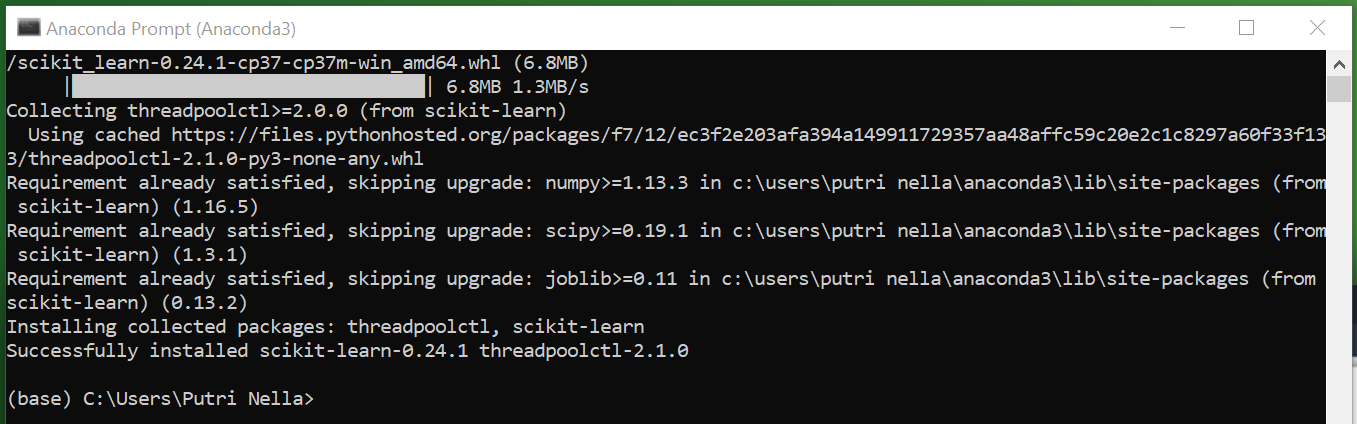
\includegraphics[width=.8\textwidth]{Pict/1.PNG}
\end{center}
    
\subsection{Example}
Untuk mengambil sebuah contoh, silahkan kunjungi website\\ https://scikit-learn.org/stable/tutorial/basic/tutorial.html lalu ambil salah satu contohnya seperti berikut ini:
\begin{lstlisting}[language=Python]
    import numpy as np
    from sklearn.model_selection import train_test_split
    from sklearn.linear_model import PoissonRegressor
    from sklearn.experimental import enable_hist_gradient_boosting 
    from sklearn.ensemble import HistGradientBoostingRegressor
    
    n_samples, n_features = 1000, 20
    rng = np.random.RandomState(0)
    X = rng.randn(n_samples, n_features)
    # positive integer target correlated with X[:, 5] with many zeros:
    y = rng.poisson(lam=np.exp(X[:, 5]) / 2)
    X_train, X_test, y_train, y_test = train_test_split(X, y, random_state=rng)
    glm = PoissonRegressor()
    gbdt = HistGradientBoostingRegressor(loss='poisson', learning_rate=.01)
    glm.fit(X_train, y_train)
    gbdt.fit(X_train, y_train)
    print(glm.score(X_test, y_test))
    print(gbdt.score(X_test, y_test))
\end{lstlisting}
Jika di running, maka akan seperti ini hasilnya:
\begin{center}
    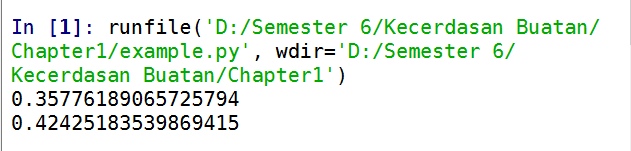
\includegraphics[width=.8\textwidth]{Pict/hasil1.PNG}
\end{center}

\subsection{Loading an example dataset}
\begin{lstlisting}[language=Python]
    from sklearn import datasets #mengimport class dataset dari scikit learn library
    iris = datasets.load_iris() #memuat dan memasukkan dataset iris ke variabel bernama iris
    digits = datasets.load_digits() #memuat dan memasukkan dataset digits ke variabel digits
    print(digits.data) #memberikan akses ke fitur yang dapat digunakan untuk mengklasifikasikan sample digit dan menampilkan di console
    digits.target #memberikan informasi tentang data yang berhubungan atau juga dapat dijadikan sebagai label
    digits.images[0] #Data selelu berupa array 2D, shape(n.samples, n.features), meskipun data aslinya mungkin memiliki bentuk yang berbeda
\end{lstlisting}
Hasilnya:
\begin{center}
    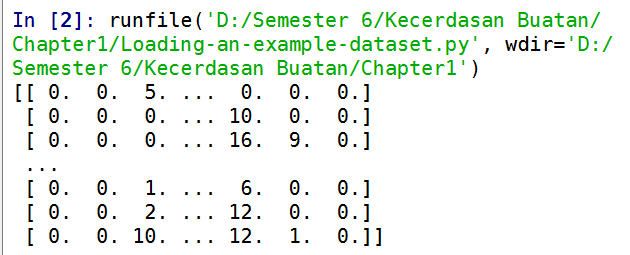
\includegraphics[width=.8\textwidth]{Pict/hasil2.PNG}
\end{center}

\subsection{Learning and predicting}
\begin{lstlisting}[language=Python]
    from sklearn import svm #perintahnuntuk mengimport class svm dari packaged sklearn
    digits = datasets.load_digits() #memuat dan memasukkan dataset digits ke variable digits
    clf = svm.SVC(gamma=0.001, C=100.) #clf sebagai estimator/parameter, svm.SVC sebagai class, gamma sebagai parameter untuk menetapkan nilai secara manual
    clf.fit(digits.data[:-1], digits.target[:-1]) #clf sebagai estimator/parameter, f i t sebagai metode, digits.data sebagai item, [:1] sebagai syntax pythonnya dan menampilkan outputannya
    print(clf.predict(digits.data[-1:])) #clf sebagai estimator/parameter, predict sebagai metode lainnya, digits.data sebagai item dan menampilkan outputannya
\end{lstlisting}
Hasilnya:
\begin{center}
    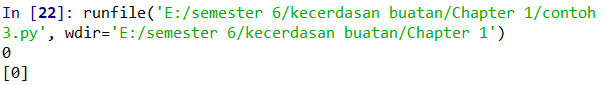
\includegraphics[width=.8\textwidth]{Pict/hasil3.PNG}
\end{center}

\subsection{Model persistence}
\begin{lstlisting}[language=Python]
    from sklearn import svm, datasets #menginport class dataset dari scikit learn library
    clf = svm.SVC(gamma=0.001, C=100.) #memanggil class SVC dan menset argumen constructor SVC serta ditampung di variabel clf
    X, y = datasets.load_iris(return_X_y=True) #meload datasets iris dan ditampung di variabel x untuk data dan y untuk target
    clf.fit(X, y) #memanggil method fit untuk melakukan training data dengan argumen data dan target dari datasets iris
    
    
    #Pickle
    import pickle
    s = pickle.dumps(clf)
    clf2 =pickle.loads(s)
    print(clf.predict(X[0:1]))
    
    #Joblib
    from joblib import dump, load
    dump(clf, '1184038.joblib')
    clf3 = load('1184038.joblib')
    print(clf3.predict(X[0:1]))
 \end{lstlisting}
 Hasilnya:
 \begin{center}
    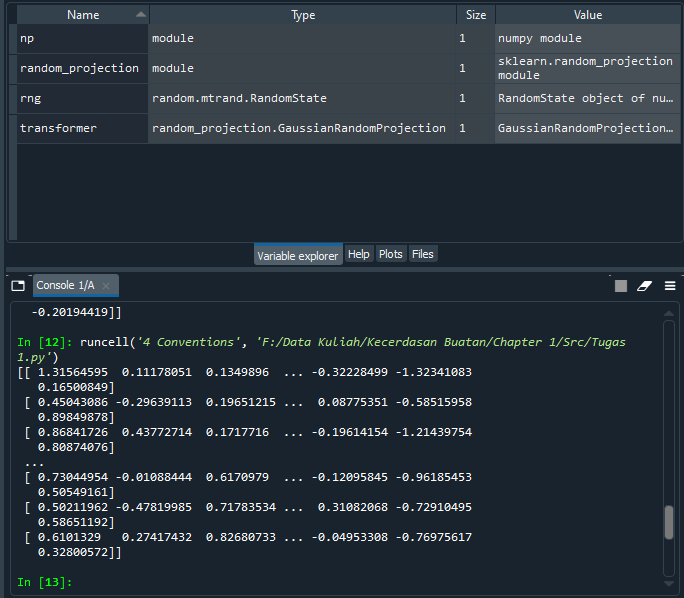
\includegraphics[width=.8\textwidth]{Pict/hasil4.PNG}
\end{center}
Selain itu, ia juga menghasilkan sebuah file joblib yang otomatis ada di dalam folder jika kita running
 \begin{center}
    
\includegraphics[width=.8\textwidth]{Pict/joblib.PNG}
\end{center}

\subsection{Conventions}
\begin{lstlisting}[language=Python]
    import numpy as np
    from sklearn import random_projection
    rng = np.random.RandomState(0)
    X = rng.rand(10, 2000)
    X = np.array(X, dtype='float32')
    print(X.dtype)
    transformer = random_projection.GaussianRandomProjection()
    X_new = transformer.fit_transform(X)
    print(X_new.dtype)
    
    from sklearn import datasets
    from sklearn.svm import SVC
    iris = datasets.load_iris()
    clf = SVC(gamma=0.001, C=100.)
    clf.fit(iris.data, iris.target)
    print(list(clf.predict(iris.data[:3])))
    clf.fit(iris.data, iris.target_names[iris.target])
    print(list(clf.predict(iris.data[:3])))

    #refiting and updatingparameter
    import numpy as np
    from sklearn.datasets import load_iris
    from sklearn.svm import SVC
    X, y = load_iris(return_X_y=True)
    clf = SVC()
    clf.set_params(kernel='linear').fit(X, y)
    print(clf.predict(X[:5]))
    clf.set_params(kernel='rbf').fit(X, y)
    print(clf.predict(X[:5]))
    
    #multiclass vc multilabel fitting
    from sklearn.svm import SVC
    from sklearn.multiclass import OneVsRestClassifier
    from sklearn.preprocessing import LabelBinarizer
    X = [[1, 2], [2, 4], [4, 5], [3, 2], [3, 1]]
    y = [0, 0, 1, 1, 2]
    classif = OneVsRestClassifier(estimator=SVC(random_state=0))
    print(classif.fit(X, y).predict(X))
    y = LabelBinarizer().fit_transform(y)
    print(classif.fit(X, y).predict(X))
    from sklearn.preprocessing import MultiLabelBinarizer
    y = [[0, 1], [0, 2], [1, 3], [0, 2, 3], [2, 4]]
    y = MultiLabelBinarizer().fit_transform(y)
    print(classif.fit(X, y).predict(X))
\end{lstlisting}
Hasilnya:
\begin{center}
    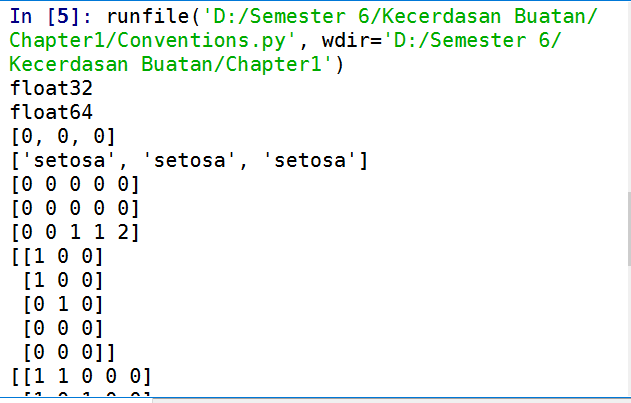
\includegraphics[width=.8\textwidth]{Pict/hasil5.PNG}
\end{center}

\section{Error}
Pada saat praktiikum, saya mengalami beberapa error, seperti:
\begin{center}
    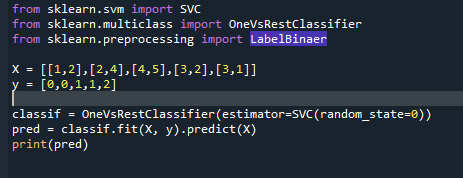
\includegraphics[width=.8\textwidth]{Pict/error1.PNG}
\end{center}
Hal ini disebabkan karena adanya variabel yang tidak dapat dipanggil. Penyelesaiannya dengan mengganti nama variabel dengan yang sudah ada dan dapat terpanggil.
\begin{center}
    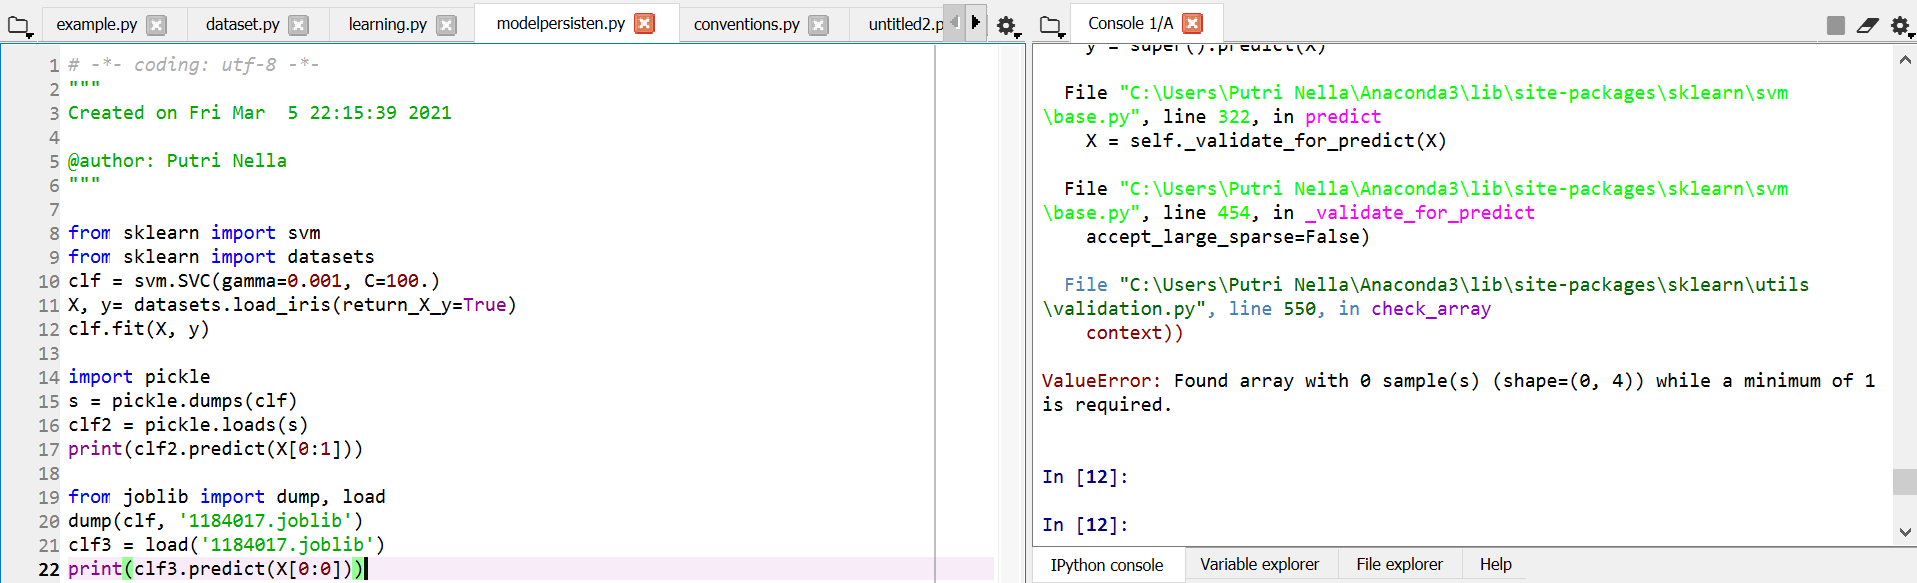
\includegraphics[width=.8\textwidth]{Pict/error2.PNG}
\end{center}
Hal ini disebabkan karena adanya kesalahan dalam penulisan kode atau tanda baca. 
\end{document}

%\section{Dinda Anik Masruro - 1184003}
\subsection{Teori}
\begin{enumerate}

	\item Definisi Kecerdasan Buatan
	\hfill\break
	Kecerdasan Buatan atau biasa disebut dengan istilah AI (Artificial Intelligence). Kecerdasan Buatan adalah salah satu bidang studi yang berhubungan dengan pemanfaatan mesin untuk memecahkan persoalan yang rumit dengan cara lebih manusiawi dan lebih bisa di pahami oleh manusia. Kecerdasan buatan makin canggih dengan kemampuan komputer dalam memperbarui pengetahuannya dengan banyaknya testing dan perkembangan target analisa. Untuk kecerdasan buatan ada banyak contoh dan jenisnya. Salah satu contoh yang paling terkenal dari Artificial Intelligence ialah Google Assistant. Google Assistant digunakan untuk kemudahan user dalam menemukan berbagai hal maupun penyetingan langsung terhadap smartphone yang digunakan dan masih banyak lagi.

	\item Sejarah dan Perkembangan
	\hfill\break
    Pada tahun 1943, pekerjaan pertama yang dikenal sebagai AI atau \textit{Artificial Intellegent} telah dikemukakan oleh Warren McCulloch dan juga Walter Pits yang dinamakan sebagai artificial neurons. Kemudian pada tahun 1955, Allen Newell dan Herbert A. Simon membuat program kecerdasan buatan pertama yang dinamakan Logic Theorist. Lalu pada tahun 1972, robot pertama dibuat di jepang dengan nama Wabot-1 dengan kecerdasan buatan. Pada tahun 1980, muncul bidang baru dari kecerdasan buatan yaitu Expert System yang membantu dalam pemberian keputusan. Kemudian pada tahun 1997, IBM deep blue mengalahkan juara catur dunia Gary Kasparov dan menjadi komputer pertama yang mengalahkannya. Tahub 2006, perusahaaan sudah mulai menerapkan kecerdasan buatan pada produknya seperti Netflix dan Twitter. Tahun 2018, Project Debater dari IBM melakuakn debat tentang topik yang kompleks dan berakhir dengan hasil memuaskan.
	
	\item Kecerdasan buatan terbagi atas beberapa metode yaitu:
	\hfill\break
	Supervised learning,  Klasifikasi, Regresi,Unsupervised Learning, Dataset, Trainingset dan juga Testingset.
	\begin{itemize}
		\item Supervised Learning
		\hfill\break
	Supervised Learning adalah sebuah tipe learning yang mempunyai variable input dan variable output, tipe ini juga menggunakan satu algoritma atau lebih dari satu algoritma yang digunakan untuk mempelajari fungsi  pemetaan dari input ke output.
		\item Klasifikasi
		\hfill\break
		Klasifikasi merupakan suatu kegiatan dari penggolongan atau pengelompokkan. Tetapi secara umum klasifikasi merupakan suatu kegiatan yang dapat mengelompokkan benda-benda yang memiliki beberapa ciri-ciri yang sama dan memisahkan benda yang tidak sama. 
		\item Regresi
		\hfill\break
        Regresi adalah metode analisis statistik yang digunakan untuk dapat melihat efek antara dua atau lebih variabel. Hubungan variabel dalam pertanyaan adalah fungsional yang diwujudkan dalam bentuk model matematika. Dalam analisis regresi, variabel dibagi menjadi dua jenis, yaitu variabel respons atau yang biasa disebut variabel dependen dan variabel independen atau dikenal sebagai variabel independen. Ada beberapa jenis analisis regresi, yaitu regresi sederhana yang mencakup linear sederhana dan regresi non-linear sederhana dan regresi berganda yang mencakup banyak linier atau non-linear berganda. Analisis regresi digunakan dalam pembelajaran mesin pembelajaran dengan metode pembelajaran terawasi.
		\item Unsupervised Learning 
		\hfill\break
        Unsupervised Learning merupakan pelatihan algoritma kecerdasan buatan (AI) menggunakan informasi yang tidak diklasifikasikan atau diberi label dan memungkinkan algoritma untuk bertindak atas informasi tersebut tanpa bimbingan. Dalam Unsupervised Learning, sistem AI dapat mengelompokkan informasi yang tidak disortir berdasarkan persamaan dan perbedaan meskipun tidak ada kategori yang disediakan.
		\item Data set
		\hfill\break
        Data set adalah objek yang merepresentasikan data dan relasinya di memory. Strukturnya mirip dengan data di database. Dataset berisi koleksi dari datatable dan datarelation.
		\item Training Set
		\hfill\break
    	Training set merupakan bagian dari data set yang di latih untuk membuat prediksi atau menjalankan fungsi dari algoritma ML lain sesuai dengan masing-masing. Memberikan instruksi melalui algoritma sehingga mesin yang di praktikkan dapat menemukan korelasinya sendiri.	
		\item Testing Set
		\hfill\break
        Testing set adalah bagian dari data set yang di uji untuk melihat akurasinya, atau dengan kata lain untuk melihat kinerjanya.
	\end{itemize}
\end{enumerate}
\subsection{Praktek}
\begin{enumerate}
	\item Instalasi Library scikit dari Anaconda, mencoba kompilasi dan uji coba ambil contoh kode dan lihat variabel explorer
	\hfill\break
	\begin{figure}[h]
		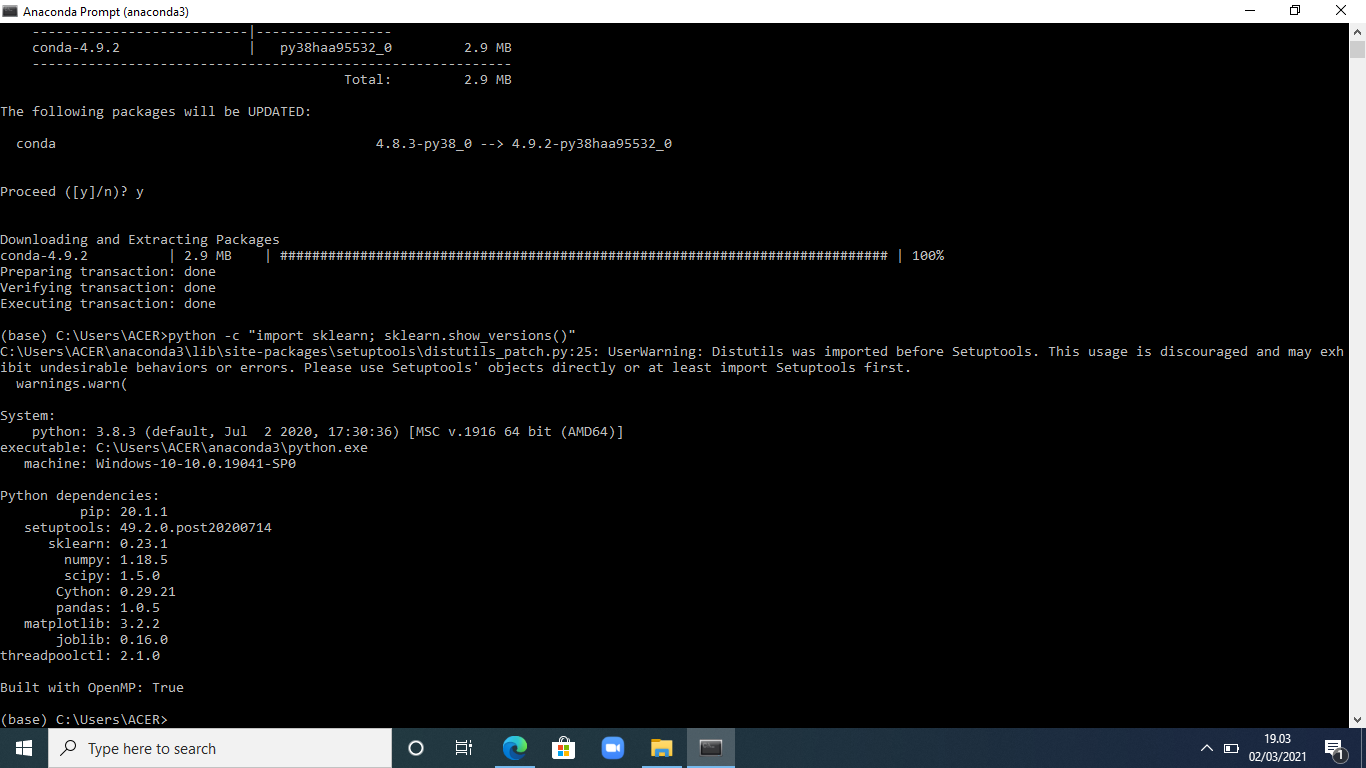
\includegraphics[width=10cm]{figures/1184003/chapter1/1.png}
		\centering
		\caption{Instalasi Library Scikit Learn}
	\end{figure}
	\begin{figure}[h]
		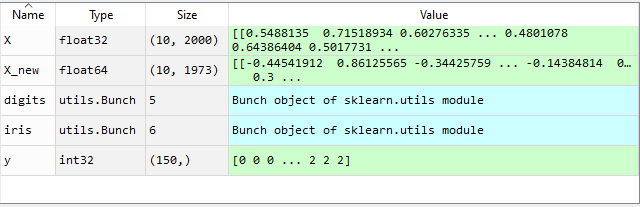
\includegraphics[width=10cm]{figures/1184003/chapter1/2.PNG}
		\centering
		\caption{Isi Variabel Explorer}
	\end{figure}
	\newpage\item Uji coba loading an example dataset
	\hfill\break
\lstinputlisting[firstline=7, lastline=16]{src/tugas1.py}
\item Uji coba Learning dan predicting
	\hfill\break
	\lstinputlisting[firstline=17, lastline=32]{src/tugas1.py}
\item Uji coba Model Persistence
	\hfill\break
	\lstinputlisting[firstline=35, lastline=63]{src/tugas1.py}	
	\item Uji coba Conventions
	\hfill\break
	\lstinputlisting[firstline=64, lastline=82]{src/tugas1.py}
	\end{enumerate}
	\subsection{Penanganan Error}
\begin{enumerate}
	\item ScreenShoot Error
	\begin{figure}[h]
		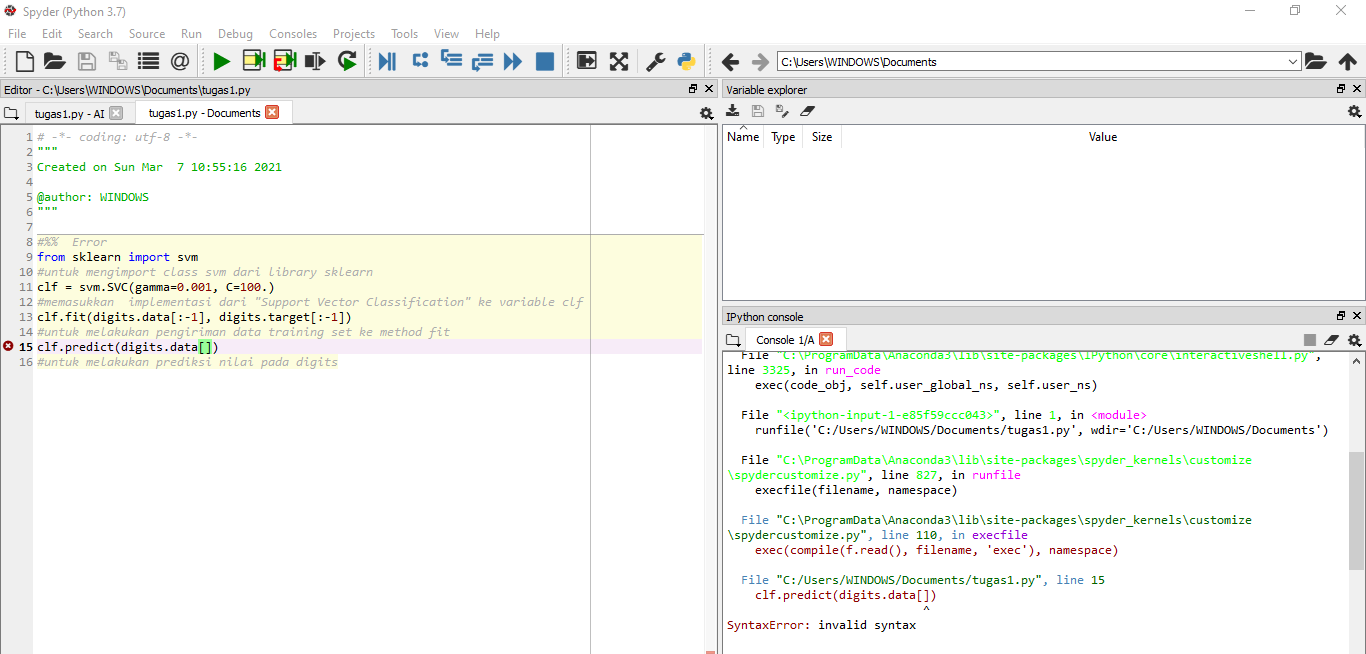
\includegraphics[width=10cm]{figures/1184003/chapter1/3.PNG}
		\centering
		\caption{Name Error}
	\end{figure}
	\newpage\item Tuliskan Kode Error dan Jenis Error
	\hfill\break
	\lstinputlisting[firstline=83, lastline=91]{src/tugas1.py}
\hfill\break
	\item Cara Penangan Error
\hfill\break Tambahkan prediksi nilainya agar kode program dapat terbaca
	\end{enumerate}
	\subsection{Bukti Tidak Plagiat}
\begin{figure}[h]
	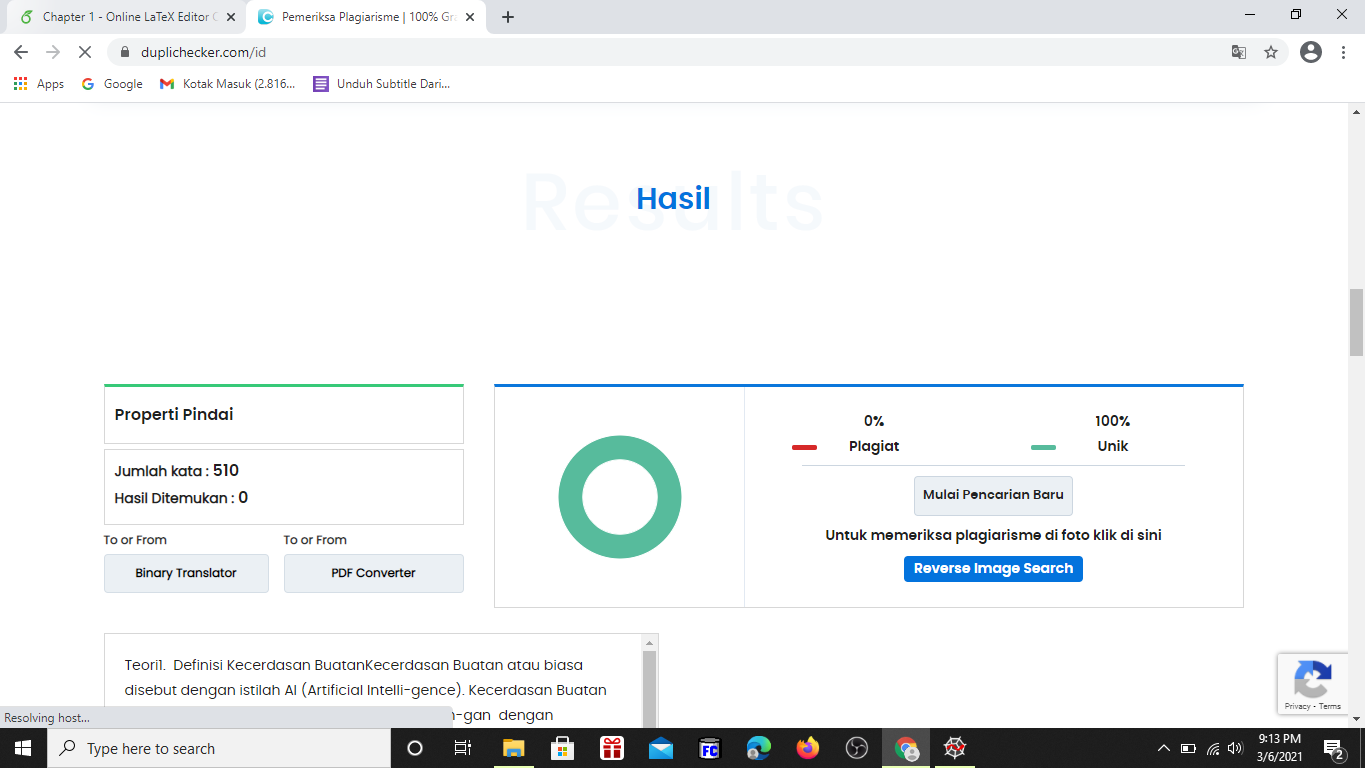
\includegraphics[width=10cm]{figures/1184003/chapter1/4.png}
	\centering
	\caption{Bukti Tidak Melakukan Plagiat Chapter 1}
\end{figure}
%\section{1184006 - Murnia Lestari}
\subsection{Teori}
\begin{enumerate}

	\item Definisi Kecerdasan Buatan
	\hfill\break
	Kecerdasan Buatan atau Artifical Inteligence yang terdiri dari kata cerdas dan buatan. Cerdas artiya cepat dan tepat.  Sedangkan buatan artinya sesuatu yang sengaja dibuat dengan tujuan tertentu. Jadi kecerdasan buatan merupakan sebuah sistem yang disimulasikan dari kecerdasan yang dipunyai oleh manusia. Sehingga sistem ini akan melakukan pelkerjaan-pekerjaan yang umumnya dikerjakan oleh manusia secara cepat dan tepat seperti yang dilakukan oleh manusia. Point-point penting yang terdapat  dalam proses kecerdasan buatan adalah learning,reasoning dan self correction.

	\item Sejarah dan Perkembangan
	\hfill\break
Kecerdasan buatan bermula pada tahun 1940-an yang bermula dari kemunculan komputer. Kemudia pada tahun 1943 McMulloh dan Pitts pada tahun 1943 mempunyai usul untuk membuat model matematis yang bernama percepton dari neurin yang ada didalam otak. Pada tahun 1950 terbuatlah mesin turing yang mencoba menjawab “dapatkah computer berpikir” yang terdapat pada paper Alan Turing. Pada tahun 1955 akhir,Newell dan simon mengembangkan The Logic Theorist yaitu program kecerdasan buatan yang pertama. Pada tahun 1956 dari Massacuhetts Institute of Technology yaitu John McCharty yang dianggap sebagai bapak dari kecerdasan buatan atau AI menyelenggarakan konferensi untuk para ahli komputer dengan nama “ The Dartmouth summer research project on artifical intelligence. Pada tahun 1960-1970 muncullah “classical AI” yang merupakan diskusi mengenai bagaimana komputer dapat meniru dengan detail kemmapuan otak manusia. Dan pada tahun 1980 merupakan titik dimna kecerdasan buatan berkembang karena komputer dapat diperoleh dengan harga yag lebih murah.
	

	\item Kecerdasan buatan terbagi atas beberapa metode yaitu:
	\hfill\break
	Supervised learning,  Klasifikasi, Regresi,Unsupervised Learning, Dataset, Trainingset dan juga Testingset.
	\begin{itemize}
		\item Supervised Learning
		\hfill\break
	Supervised Learning	merupakan algoritma yang memiliki attribut tambahan seperti x dan y yang ingin diprediksi.
		\item Klasifikasi
		\hfill\break
		Klasifikasi merupakan sampel yang dimiliki oleh dua atau lebih kelas yang dikelompokkan yang disesuaikan berdasarkan ukuran kemiripan atau jarak yang melekat. 
		\item Regresi
		\hfill\break
Regresi	merupakan sebuah prediksi apabila hasil atau output yang diinginkan terdiri dari satu atau lebih variable contionous.
		\item Unsupervised Learning 
		\hfill\break
Unsupervised Learning  merupakan	algoritma yang tidak memiliki attribut tambahan yang akan diprediksi
		\item Data set
		\hfill\break
Data set	merupakan kondisi dimana hanya terdapat inputan data tanpa memiliki viariasi output yang sesuai
		\item Training Set
		\hfill\break
	Training Set	merupakan bagian dari data set yang digunakan untuk mempelajari beberapa properti		
		\item Testing Set
		\hfill\break
Testing Set	merupakan bagian data set yang digunakan untuk pengujian dari properti yang dipelajari
	\end{itemize}
\end{enumerate}
\subsection{Praktek}
\begin{enumerate}
	\item Instalasi Library scikit dari Anaconda, mencoba kompilasi dan uji coba ambil contoh kode dan lihat variabel explorer
	\hfill\break
	\begin{figure}[h]
		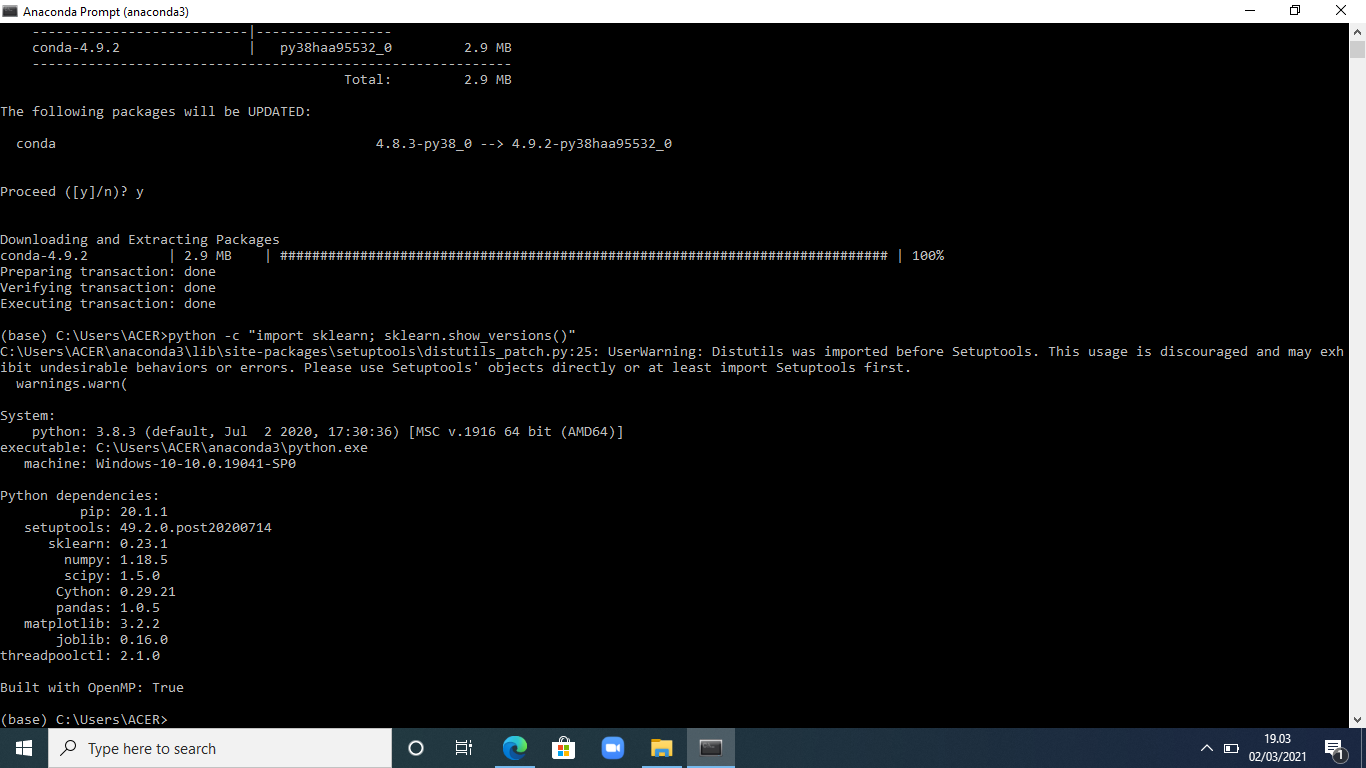
\includegraphics[width=10cm]{figures/1184006/chapter1/01.png}
		\centering
		\caption{Instalasi Library Scikit Learn}
	\end{figure}
	\begin{figure}[h]
		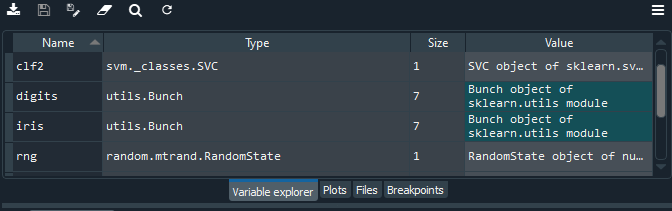
\includegraphics[width=10cm]{figures/1184006/chapter1/02.PNG}
		\centering
		\caption{Isi Variabel Explorer}
	\end{figure}
	\newpage\item Uji coba loading an example dataset
	\hfill\break
\lstinputlisting[firstline=7, lastline=16]{src/1184006/chapter1/tugas1.py}
\item Uji coba Learning dan predicting
	\hfill\break
	\lstinputlisting[firstline=17, lastline=32]{src/1184006/chapter1/tugas1.py}
\item Uji coba Model Persistence
	\hfill\break
	\lstinputlisting[firstline=35, lastline=63]{src/1184006/chapter1/tugas1.py}
	\item Uji coba Conventions
	\hfill\break
	\lstinputlisting[firstline=64, lastline=82]{src/1184006/chapter1/tugas1.py}
	\end{enumerate}
	\subsection{Penanganan Error}
\begin{enumerate}
	\item ScreenShoot Error
	\begin{figure}[h]
		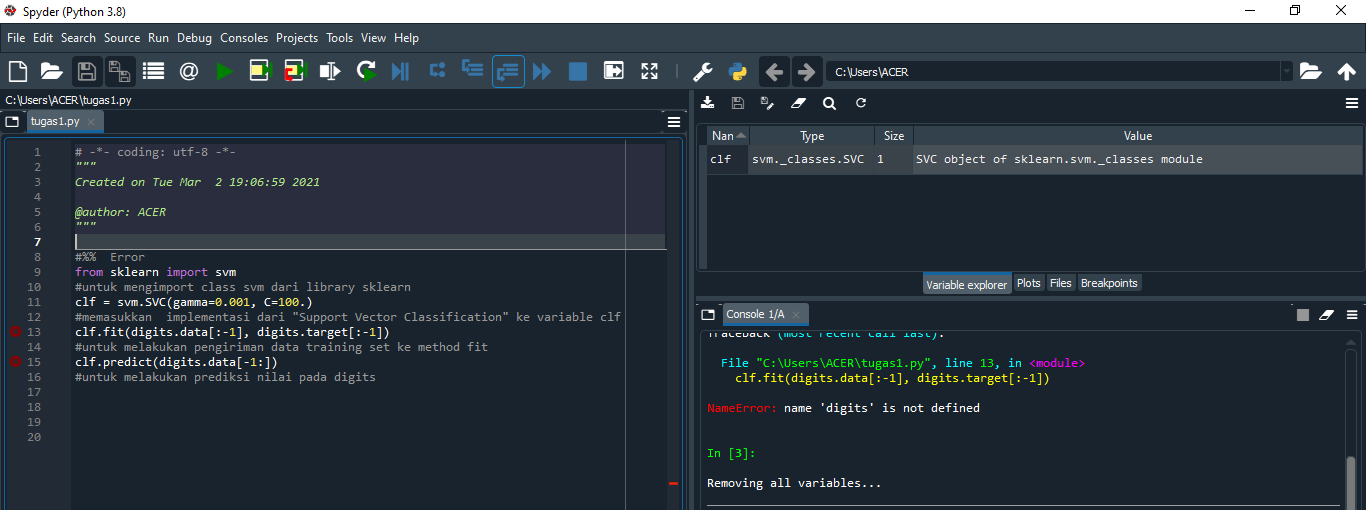
\includegraphics[width=10cm]{figures/1184006/chapter1/03.PNG}
		\centering
		\caption{Name Error}
	\end{figure}
	\newpage\item Tuliskan Kode Error dan Jenis Error
	\hfill\break
	\lstinputlisting[firstline=83, lastline=91]{src/1184006/chapter1/tugas1.py}
\hfill\break
	\item Cara Penangan Error
\hfill\break Tambahkan variabel digits agar kode program dapat terbaca
	\end{enumerate}
	\subsection{Bukti Tidak Plagiat}
\begin{figure}[h]
	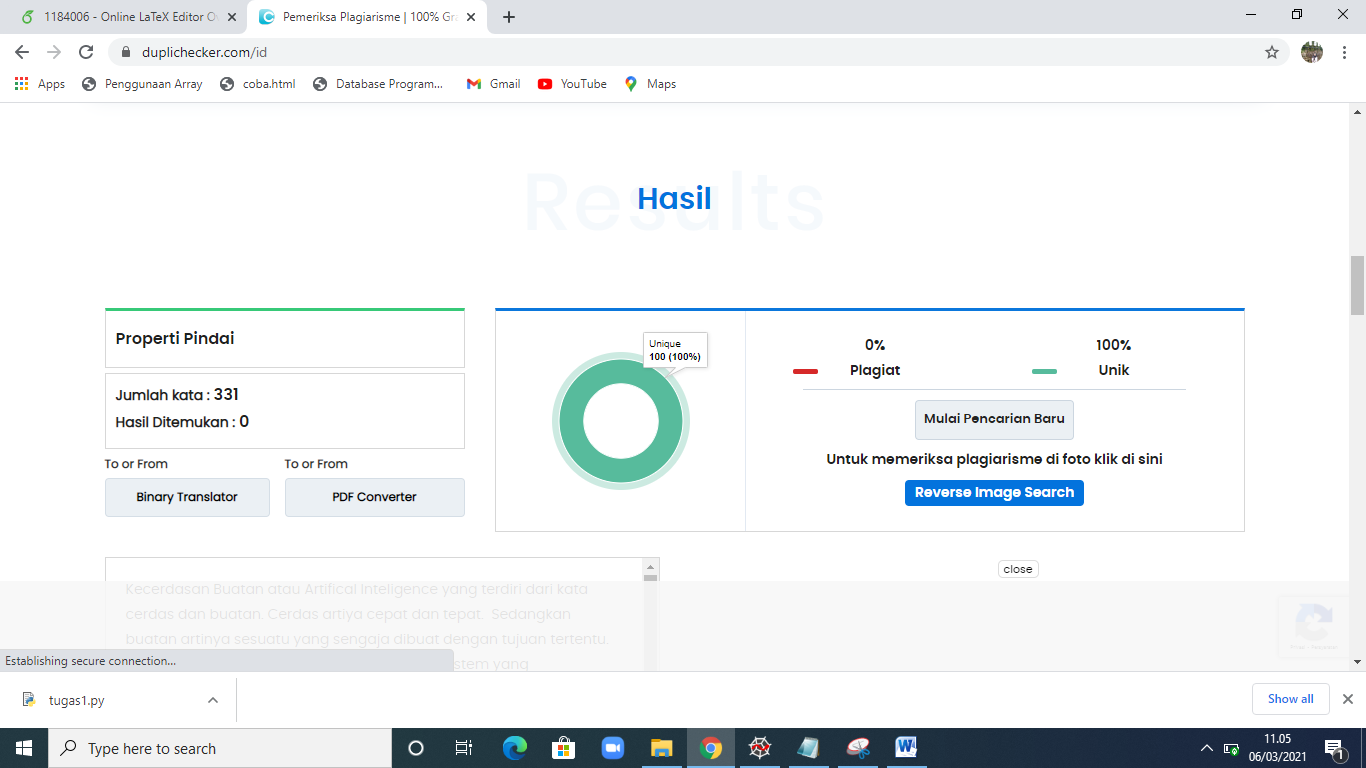
\includegraphics[width=10cm]{figures/1184006/chapter1/04.png}
	\centering
	\caption{Bukti Tidak Melakukan Plagiat Chapter 1}
\end{figure}
%\section{1184071 - Annisa Khairani Febrianti}
\subsection{Teori}
\begin{enumerate}
	\item Definisi Kecerdasan Buatan (AI)
	\hfill\break
	Kecerdasan Buatan atau \textit{Artificial Intelligence} (AI) merupakan teknik meniru kecerdasan yang dimiliki oleh makhluk hidup maupun benda mati untuk menyelesaikan suatu masalah. Atau dapat di definisikan sebagai salah satu cabang Ilmu pengetahuan yang berkaitan dengan pemanfaatan mesin untuk menyelesaikan persoalan rumit dengan menggunakan cara yang lebih manusiawi. Adapun contoh sederhana penerapan kecerdasan buatan adalah SIRI, bagi pengguna iphone atau \textit{IOS} pasti sudah tidak asing dengan SIRI yang
    seringkali diartikan sebagai asisten pribadi pengguna IOS dalam melakukan hal-hal tertentu untuk penggunanya.

	\item Perkembangan dan Sejarah AI
	\hfill\break
	Pada tahun 1956 merupakan tahun pertama kali muncul istilah AI atau \textit{Artificial Intellegent} yang dikemukakan oleh \textbf{John McCarthy} di Konferensi Darthmouth.Penggunaan AI begitu popular dari tahun ke tahun. Pada tahun 1950-an merupakan tahap dimana riset awal proyek AI yang tujuan untuk eksplorasi topik penyelesaian persoalan dan metode simbolik.Selanjutnya Pada tahun 1959, Dari IBM yang bernama \textbf{Nathaniel Rochester} bersama beberapa mahasiswa lainnya mengeluarkan program kecerdasan buatan yaitu \textit{Geometry Theorm Prover}. Lalu pada tahun 1960-an Departemen Pertahanan yang berasal dari Amerika Serikat memiliki keinginan dalam melatih dan mengembangkan komputer supaya memiliki nalar yang menyerupai manusia secara dasar. Kemudian Pada tahun 1963, program yang mampu menyelesaikan masalah integral tertutup untuk mata kuliah Kalkulus dibuat dengan \textbf{James Slagle}. Pada tahun 1970-an, adanya suatu keberhasilan proyek DARPA \textit{(Defence Advanced Research Project Agency)} dengan mampu menyelesaikan studi kasus tentang pemetaan jalan. Selanjutnya Pada tahun 1986, program analogi yang digunakan dalam pemecahan masalah analogi geometris yang ada pada tes IQ dibuatan oleh \textbf{Tom Evan}. Dari tahun 1980an AI kemudian mulai berkembang dibidang idustri dan mulai berkiprah hingga saat ini dimana para ilmuan berlomba-lomba untuk menciptakan AI yang bermanfaat pada kehidupan sekarang atau dimasa depan nanti. Setelah itu pada awal abad ke 21 atau lebih tepatnya pada tahun 2003, DARPA berhasil untuk menciptakan asisten pribadi yang cerdas. Sejak saat itu lah teknologi AI terus berkembang sangat bagus dan sampai saat ini AI tersebutlebih menjurus pada program yang lebih detail dan kompleks dengan penerapan struktur algoritma dari pembelajaran secara mendalam atau \textit{deep learning} yaitu AI yang dikembangkan bisa mengerjakan persoalan dan memberi solusi yang lebih kompleks dengan kondisi yang lebih beragam.

	\item Kecerdasan buatan (AI) terbagi menjadi beberapa metode yaitu:
	\hfill\break
	Supervised learning,  Klasifikasi, Regresi,Unsupervised Learning, Dataset, Trainingset dan juga Testingset.
	\begin{itemize}
		\item Supervised Learning
		\hfill\break
	Supervised learning merupakan suatu pembelajaran dengan adanya pengawas atau bisa disebut dengan supervisor. Supervisor merupakan suatu label yang ada di setiap data nya. Kemudian label tersebut berisi tag dari data yang ditambah ke dalam model pembelajaran mesin atau lebih trend disebut dengan \textbf{machine learning model}. Bisa diilustrasikan seperti gambar apel di tag “apel” dari masing-masing gambar tersebut apel dan gambar pir di tag “pir”dari masing-masing gambar pir. Lalu Machine learning memiliki berapa kategori berupa clasification (“apel”, “pir”, dsb) dan regression ( tinggi badan, berat badan, dsb).
		\item Klasifikasi
		\hfill\break
		Klasifikasi merupakan sampel yang dimiliki oleh dua atau lebih kelas yang dikelompokkan yang disesuaikan berdasarkan ukuran kemiripan atau jarak yang melekat. 
		\item Regresi
		\hfill\break
    Regresi	merupakan sebuah prediksi apabila hasil atau output yang diinginkan terdiri dari satu atau lebih variable contionous.
		\item Unsupervised Learning 
		\hfill\break
Unsupervised learning merupakan suatu pembelajaran tanpa adanya sebuah pengawasan dan tidak menggunakan label untuk bisa memprediksi target variable. Unsupervised learning lebih mengelompokan tentang kesamaan ataupun kemiripan dari attribut yang sudah diinputkan. Apabila attribut dan sifat dari data variable yang diproses ternyata memiliki kemiripan, maka akan dijadikan
satu kelompok (clustering). Dan akan menimbulkan beberapa bagian kelompok (cluster). Jumlah cluster bisa tidak terbatas. Dari kelompok tersebut model melabelkan, dan jika data baru akan di prediksi, itu akan diproses untuk mencocokan kelompok yang memiliki kemiripan feature. unsupervised learning tidak punya outcome spesifik seperti supervise learning karena tidak adanya sebuah label dasar.
\hfill\break
\textbf{Dapat disimpulkan Jika Supervised learning tentang atribut atau label yang sudah ada dari kategori yang diinginkan berbeda dengan unservised learning dimana unsupervised menggunakan kesamaan dari attribut yang dimiliki. Jika attribut dan sifat dari data feature yang diekstrak memiliki
kemiripan, maka akan dikelompokan kedalam \textit{(clustering)}. Sehingga hal ini
akan menimbulkan kelompok \textit{(cluster)}. Jumlah cluster bisa unlimited atau tidak terbatas}.
		\item Data Set
		\hfill\break
Data Set merupakan kumpulan sampel yang sudah dikumpulkan dan bersifat
homogen. Salah satu contohnya yaitu Seorang anak ingin bermain Voli, tetapi keputusannya untuk bermain voli tersebut tergantung pada variable yang ditentukan contohnya jarak kaki dari garis, atau tinggi net sehingga variable ini disebut dengan fitur dalam sebuah permainan.
		\item Training Set
		\hfill\break
Data yang digunakan untuk bisa melakukan klasifikasi ataupun prediksi,Dengan adanya data training maka akan didapatkan sebuah model regresi.		
		\item Testing Set
		\hfill\break
Testing Set digunakan untuk menguji kebenaran dari sebuah model data.Adapun Testing data berisi \textit{unseen example} merupakan contoh yang tidak ada didalam training set.
	\end{itemize}
\end{enumerate}
\subsection{Praktek}
\begin{enumerate}
	\item Instalasi Library scikit dari Anaconda, mencoba kompilasi dan uji coba ambil contoh kode dan lihat variabel explorer
	\hfill\break
	\begin{figure}[h]
		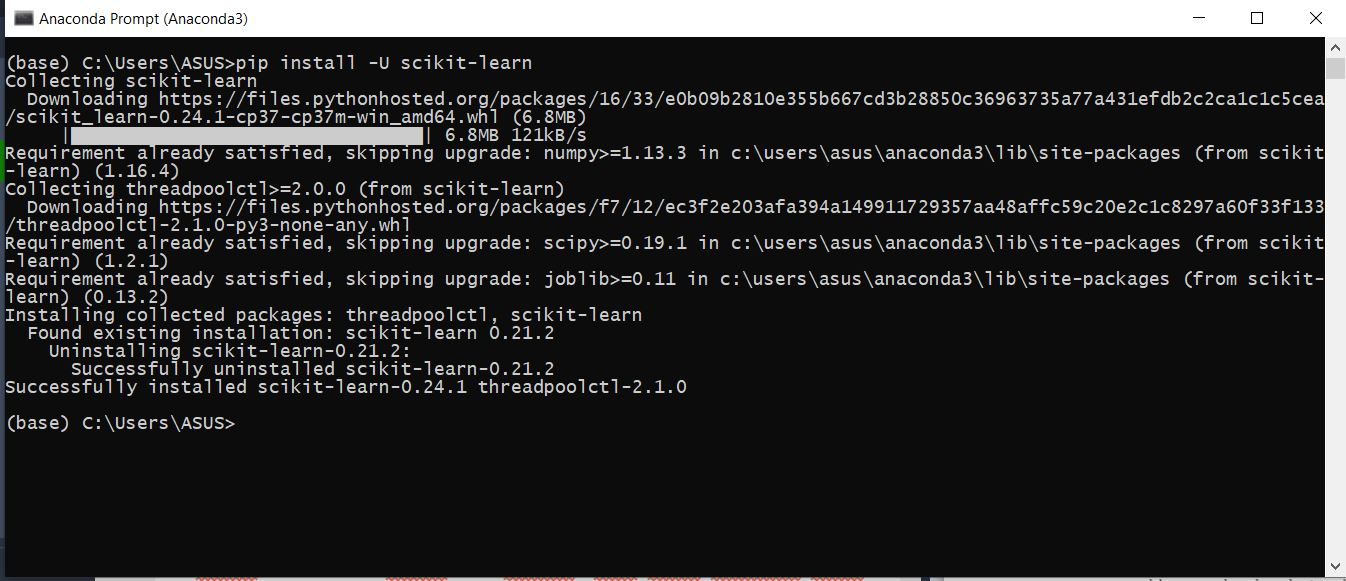
\includegraphics[width=12cm]{figures/1184071/chapter1/1.JPG}
		\centering
		\caption{Instalasi Library Scikit Learn}
	\end{figure}
	\begin{figure}[h]
		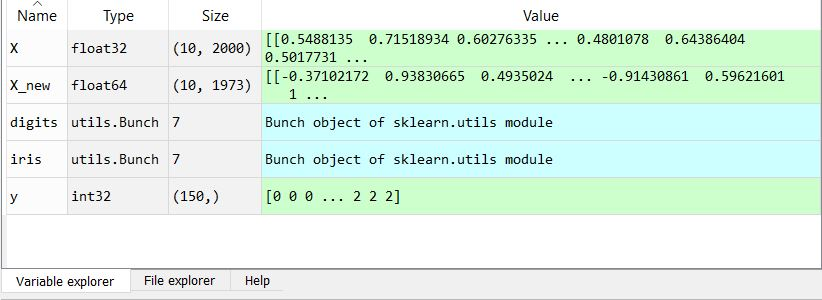
\includegraphics[width=15cm]{figures/1184071/chapter1/2.JPG}
		\centering
		\caption{Isi Variabel Explorer}
	\end{figure}
	\newpage\item Uji coba loading an example dataset
	\hfill\break
\lstinputlisting[firstline=7, lastline=16]{src/tugas1.py}
\item Uji coba Learning dan predicting
	\hfill\break
	\lstinputlisting[firstline=17, lastline=32]{src/tugas1.py}
\item Uji coba Model Persistence
	\hfill\break
	\lstinputlisting[firstline=35, lastline=63]{src/tugas1.py}	
	\item Uji coba Conventions
	\hfill\break
	\lstinputlisting[firstline=64, lastline=82]{src/tugas1.py}
	\end{enumerate}
	\subsection{Penanganan Error}
\begin{enumerate}
	\item ScreenShoot Error
	\begin{figure}[h]
		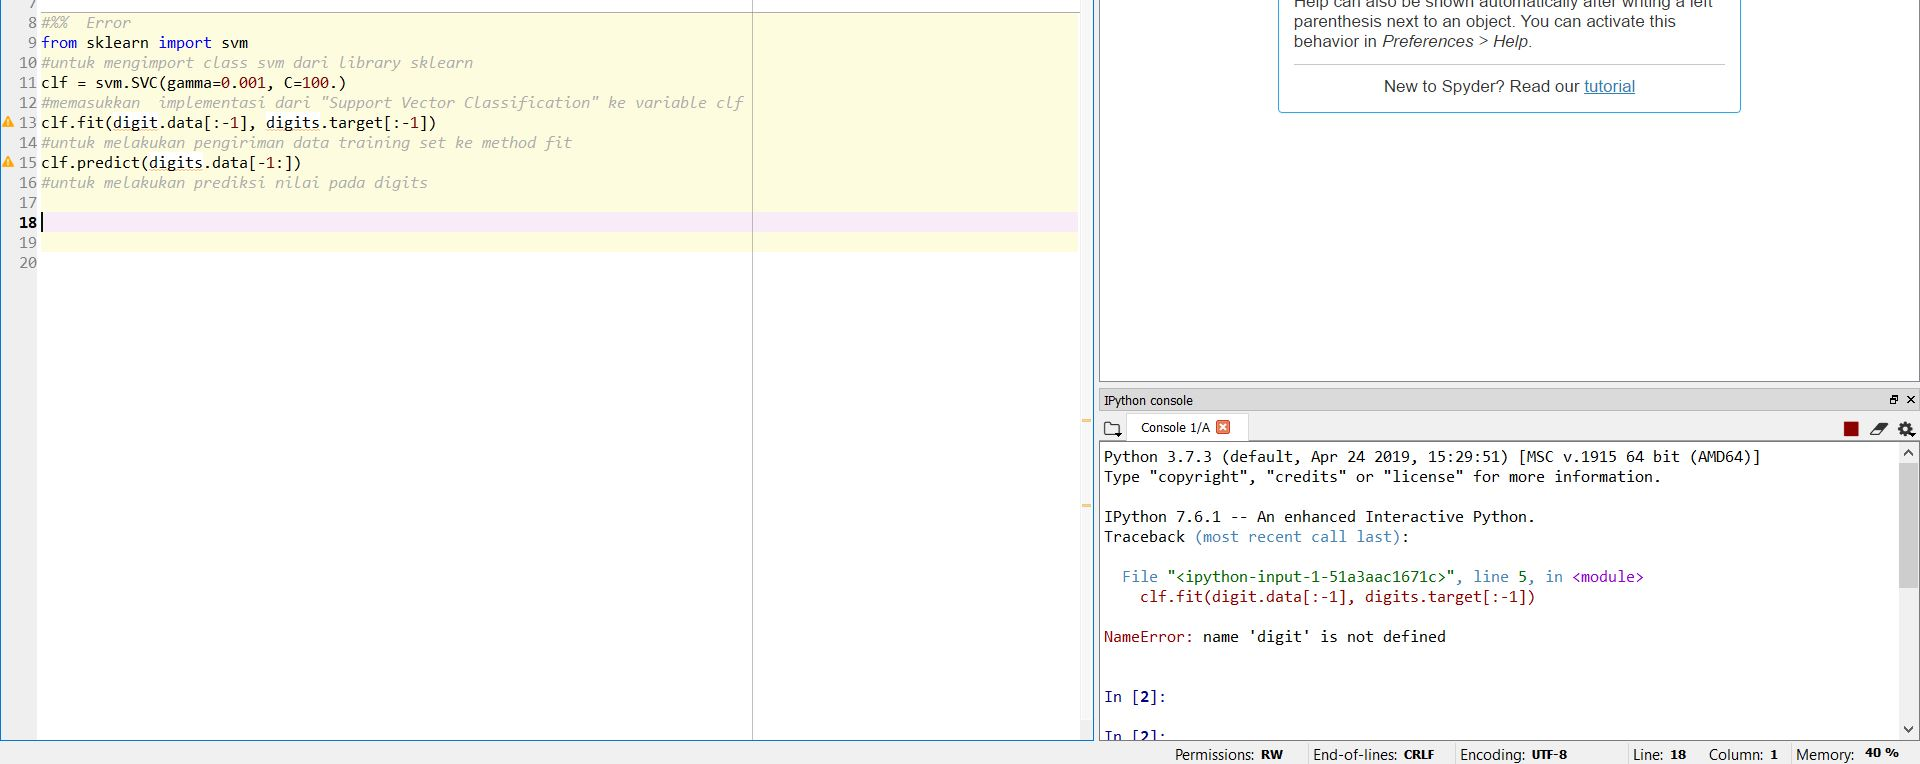
\includegraphics[width=15cm]{figures/1184071/chapter1/3.JPG}
		\centering
		\caption{Name Error}
	\end{figure}
	\newpage\item Tuliskan Kode Error dan Jenis Error
	\hfill\break
	\lstinputlisting[firstline=83, lastline=91]{src/tugas1.py}
\hfill\break
	\item Cara Penangan Error
\hfill\break Tambahkan variabel digits agar kode program dapat terbaca
	\end{enumerate}
	\subsection{Bukti Tidak Plagiarisme}
\begin{figure}[h]
	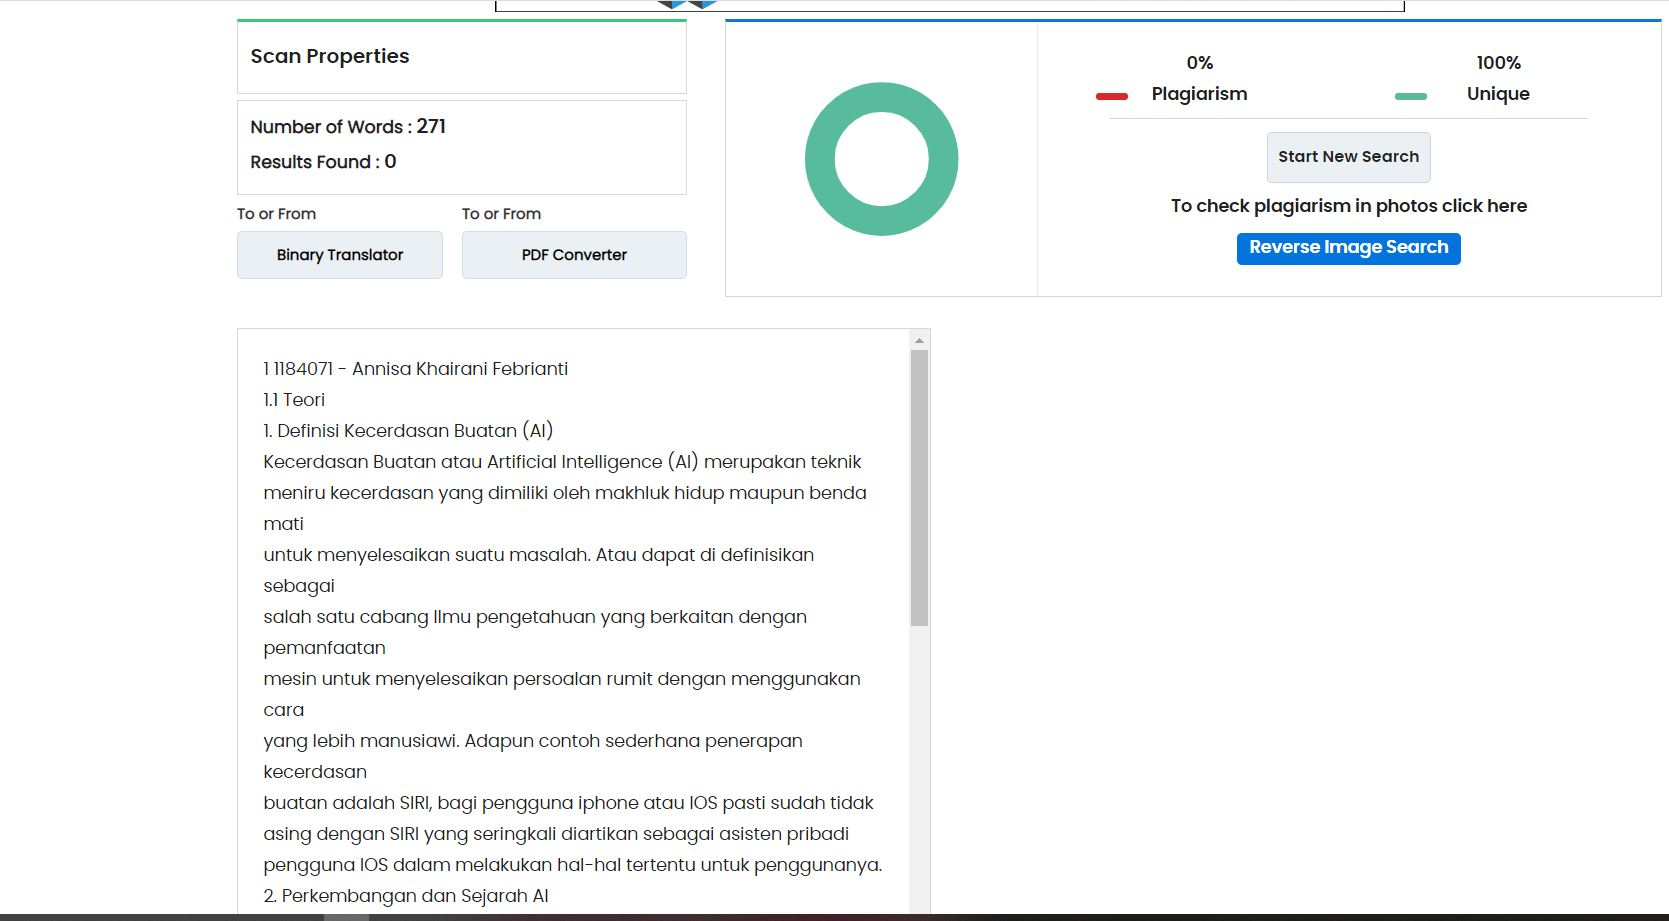
\includegraphics[width=15cm]{figures/1184071/chapter1/4.JPG}
	\centering
	\caption{Bukti Tidak Melakukan Plagiarisme Chapter 1}
\end{figure}
%\chapter{Heriyanto - 1184023}

\section{Teori}

\subsection{Definisi dan Sejarah Kecerdasan Buatan}

\subsubsection{Definisi Kecerdasan Buatan}
Kecerdasan buatan adalah sistem kecerdasan yang ditanamkan atau ditambahkan ke dalam teknologi oleh manusia, yang kemudian akan dikembangkan dalam lingkungan ilmiah atau dalam pembentukan entitas ilmiah yang ada. Kecerdasan di sini menekankan pada kemampuan memperoleh pengetahuan baru, yang dapat langsung diterapkan. Meskipun AI memiliki konotasi ilmiah, AI juga merupakan cabang dari ilmu komputer, pembelajaran, perilaku (behaviour), dan adaptasi pada mesin. \cite{purwanti2017analisis}. 

\subsubsection{Definisi Kecerdasan Buatan Menurut Para Ahli}
\begin{enumerate}
    \item Scahlkoff (1990)
    
    \par Kecerdasan Buatan merupakan bidang studi yang berusaha menerangkan dan meniru perilaku kecerdasan dalam bentuk proses komputasi.\cite{ai2011kecerdasan}
    
    \item Luger dan Stubblefield (1993)
    
    \par Kecerdasan Buatan merupakan cabang ilmu komputer yang berhubungan dengan otomatisasi perilaku yang cerdas.\cite{ai2011kecerdasan}
    
    \item Rich dan Knight (1991)
    
    \par Kecerdasan Buatan merupakan studi tentang cara membuat komputer melakukan sesuatu yang sampai saat ini, orang dapat melakukannya lebih baik.\cite{ai2011kecerdasan}
    
    \item Haag dan Keen (1996)
    
    \par Kecerdasan Buatan adalah bidang studi yang berhubungan dengan penangkapan, pemodelan, dan penyimpanan kecerdasan manusia dalam sebuah sistem teknologi sehingga sistem tersebut dapat memfasilitasi proses pengambilan keputusan yang biasanya dilakukan oleh manusia.\cite{ai2011kecerdasan}
\end{enumerate}

\subsection{Sejarah Kecerdasan Buatan}

\par Istilah kecerdasan buatan pertama kali diusulkan pada tahun 1956. Hingga saat ini, dengan peningkatan daya komputasi dan kapasitas penyimpanan, penggunaan kecerdasan buatan menjadi semakin populer. Fase penelitian awal proyek AI berlangsung sekitar tahun 1950-an, bertujuan untuk mengeksplorasi tema pemecahan masalah dan metode simbolik.

\par Pada 1960-an, Departemen Pertahanan AS juga sangat ingin mengembangkan dan melatih komputer dengan kemampuan dasar penalaran manusia. Sekitar tahun 1970-an, proyek DARPA (Defense Advanced Research Projects Agency) berhasil menyelesaikan studi kasus pemetaan jalan. Di awal abad ke-21, tepatnya tahun 2003, DARPA juga berhasil melahirkan asisten pribadi yang cerdas.

\par Setelah itu, teknologi kecerdasan buatan terus berkembang, dan hingga saat ini memasuki prosedur yang lebih detail dengan menerapkan algoritma deep learning. Di sana, kecerdasan buatan yang dikembangkan dapat melakukan tugas dan memberikan solusi yang lebih kompleks dengan kondisi yang lebih beragam.\cite{sejarahai}

\subsection{Supervised Learning dan Unsupervised Learning}

\subsubsection{Supervised Learning}

\par Supervised learning (pembelajaran terarah) adalah metode pembelajaran mesin di mana pengguna mengharapkan hasil, dan informasinya diketahui atau dimiliki oleh sistem. Artinya metode pembelajaran bekerja dengan menggunakan kembali masukan atau data pengguna dan hasil keluaran yang sebelumnya diselesaikan oleh sistem. Supervised Learning itu sendiri dapat dibagi lagi menjadi regresi dan klasifikasi.\cite{mahardhika2018analisis}

\par Regresi adalah teknik analisis yang digunakan untuk mengidentifikasi hubungan antara dua variabel atau lebih. Tujuan dari regresi adalah untuk menemukan fungsi yang memodelkan data dengan meminimalkan kesalahan atau perbedaan antara nilai prediksi dan nilai sebenarnya.

\par Klasifikasi adalah teknik yang digunakan untuk mengklasifikasikan beberapa item yang tidak berlabel ke dalam satu set kelas diskrit. Klasifikasi mencoba mempelajari hubungan antara sekumpulan variabel fitur dan variabel target. Dalam klasifikasi, variabel targetnya adalah tipe kategori.

\subsubsection{Unsupervised Learning}

\par Unsupervised Learning adalah metode lain dalam materi pembelajaran mesin, di mana tidak ada yang bisa mengetahui hasil yang diharapkan. Tujuan utama dari metode pembelajaran ini adalah agar para penggunanya dapat mengelompokkan objek-objek yang dianggap serupa pada suatu ruang atau area tertentu.\cite{unsuper}

\subsection{Data Set}

\par Kumpulan data adalah objek yang mirip dengan kamus, yang menyimpan semua data dan beberapa metadata tentang data.\cite{scikit} 

\par Saat membuat model Machine Learning, data harus dibagi menjadi satu Training Set dan satu Testing Set. Machine Learning harus diberi tahu "Data Set" mana yang akan dicapai, dan "Data Set" yang dapat digunakan untuk mencapai tujuan. "Data Set" untuk dicapai ini adalah Testing Set, dan "Data Set" untuk mencapai ini disebut Training Set.\cite{dataset}

\par Training Set adalah bagian dari Data Set yang dilatih untuk membuat prediksi atau menjalankan fungsi algoritma ML. Dengan memberikan petunjuk melalui algoritma sehingga mesin yang dilatih dapat menemukan korelasinya sendiri atau mempelajari pola dari data yang diberikan. Testing Set adalah bagian dari data set yang diuji untuk melihat akurasinya, atau dengan kata lain, untuk melihat performanya.\cite{traintest}

\section{Instalasi}

\subsection{Instalasi Scikit-Learn pada Anaconda}

\begin{enumerate}
    \item Pastikan Anaconda telah terpasang pada perangkat komputer atau laptop yang anda gunakan.
    \item Jika Anaconda belum terpasang pada perangkat anda silahkan kunjungi link berikut untuk tutorial memasang anaconda: https://docs.anaconda.com/anaconda/install/.
    \item Setelah anaconda terpasang buka command shell anaconda, dengan mengetik di start menu "Anaconda Prompt (ananconda 3)".
        \begin{figure}[H]
        \centering
        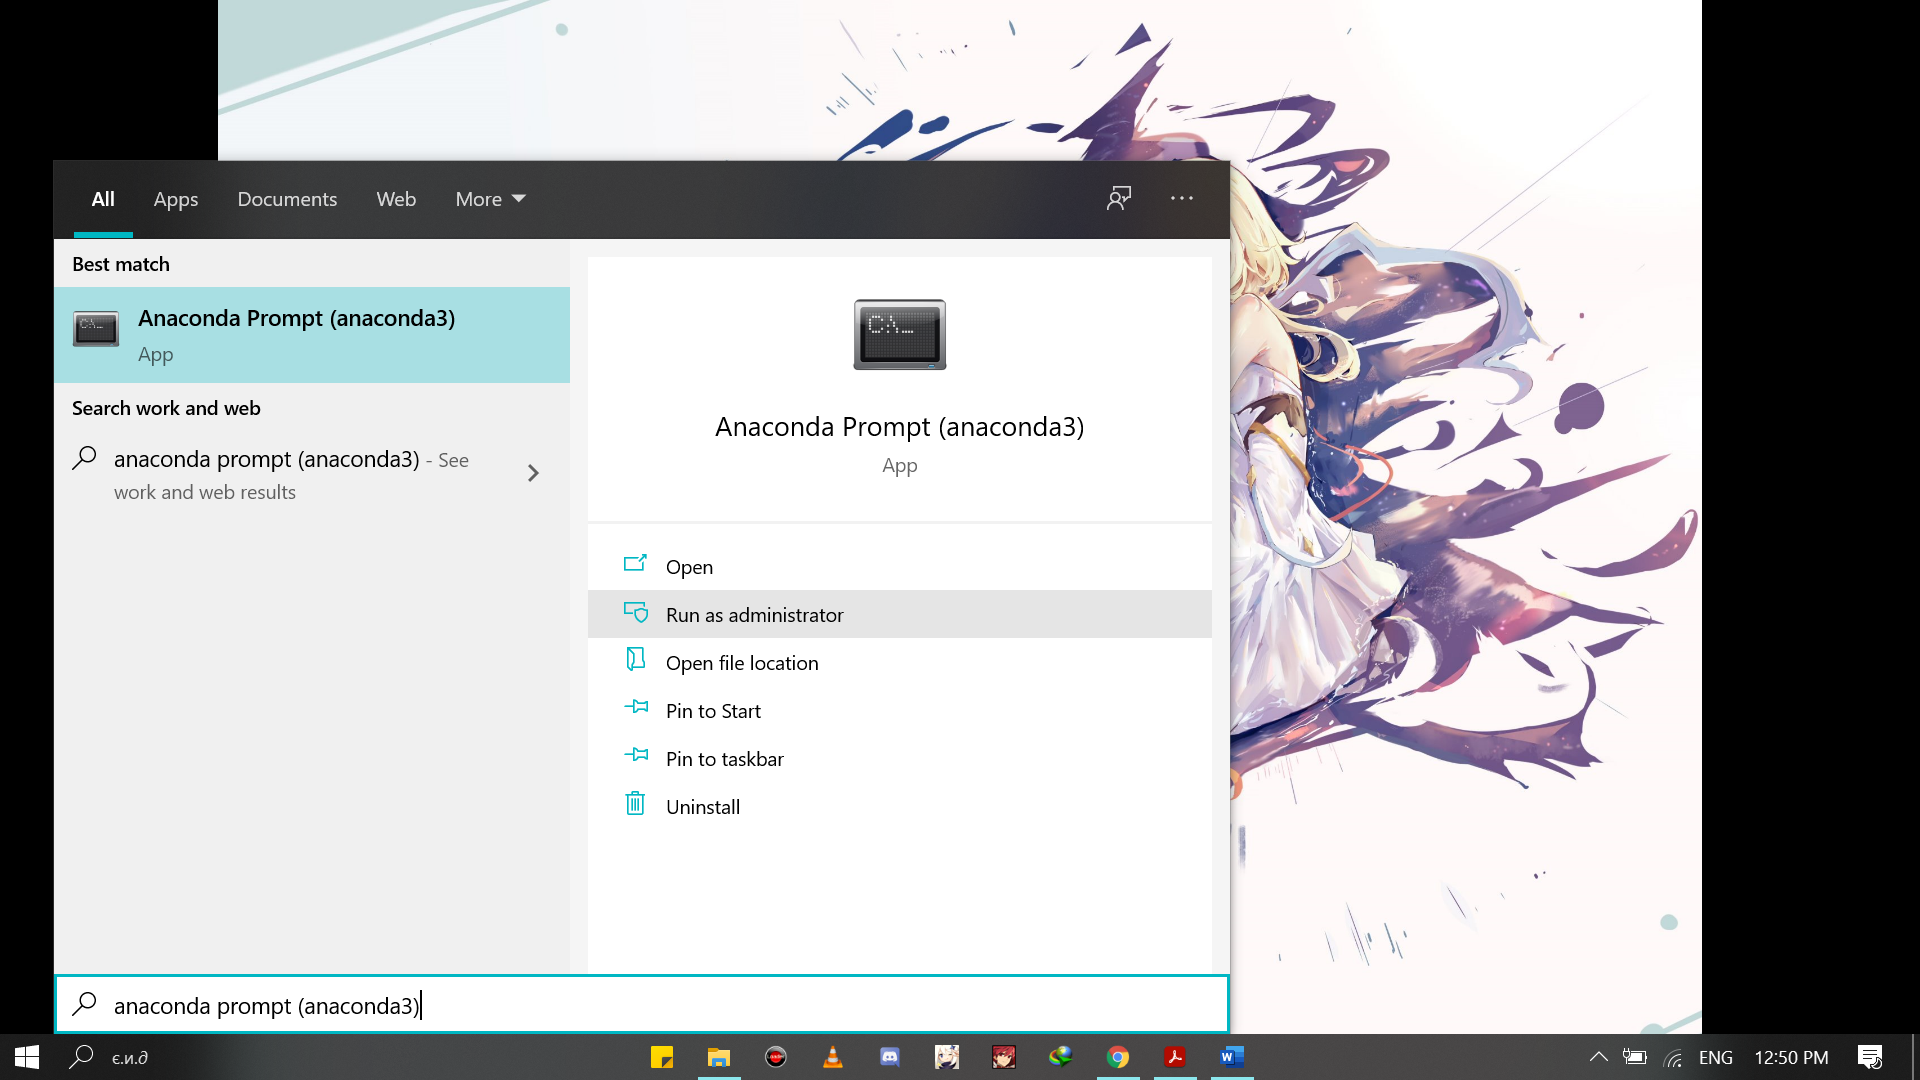
\includegraphics[width=11cm]{figures/1184023/install.png}
        \caption{Anaconda Prompt}
        \end{figure}
    \item Kemudian ketik perintah berikut untuk memasang scikit-learn library pada anaconda: conda install -c conda-forge scikit-learn, dan tunggu sampai prosesnya selesai.
        \begin{figure}[H]
        \centering
        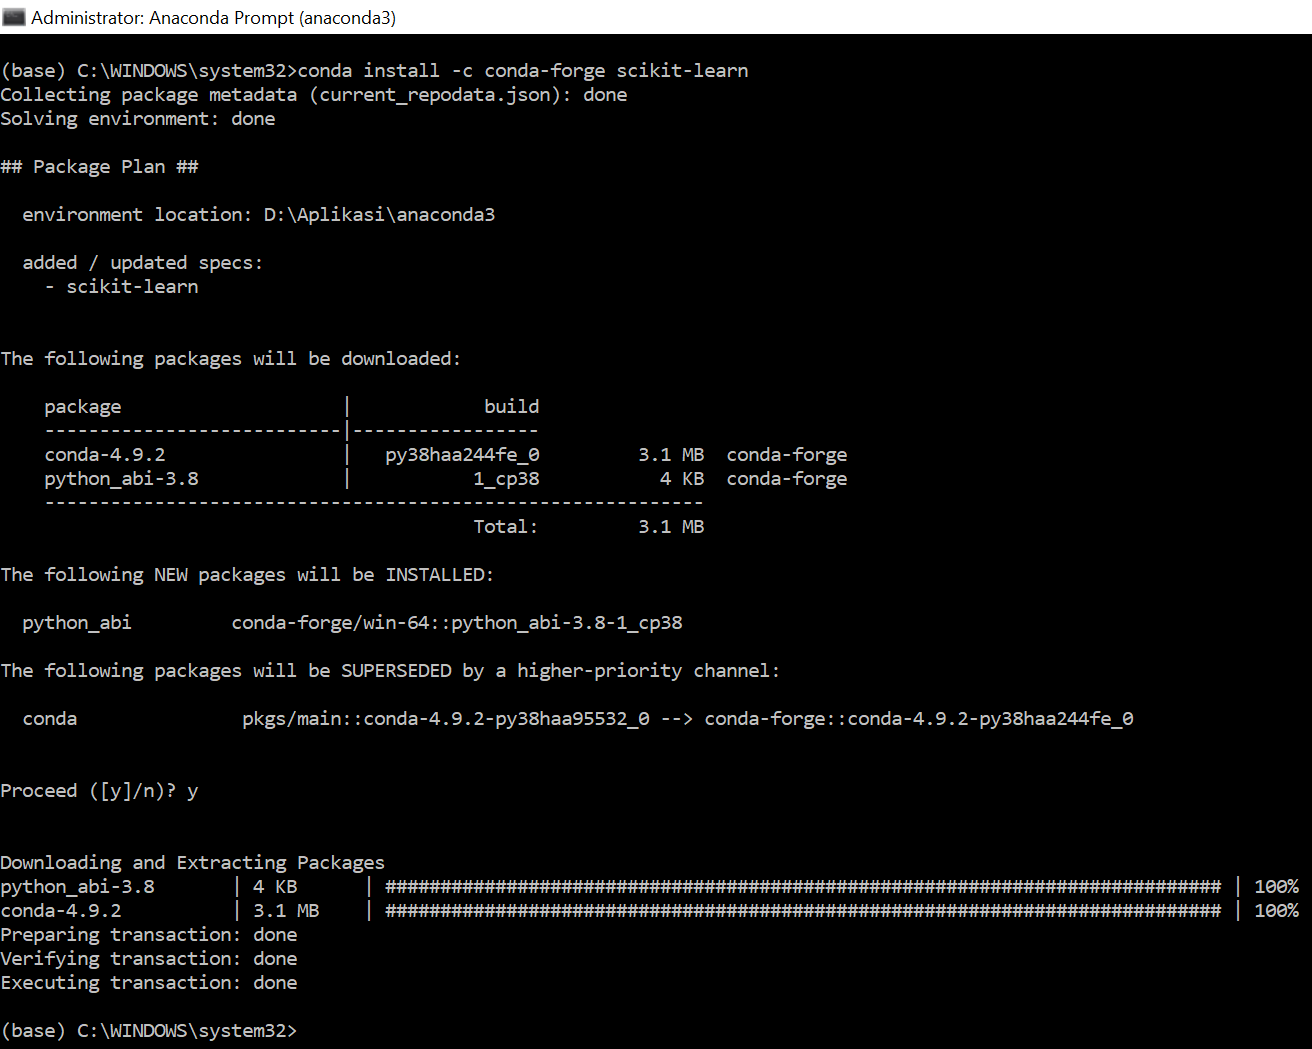
\includegraphics[width=13cm]{figures/1184023/1.PNG}
        \caption{Anaconda Prompt}
        \end{figure}
\end{enumerate}

\subsection{Loading an example dataset}

\par Scikit-learn hadir dengan beberapa dataset standar, misalnya dataset iris dan digit untuk klasifikasi dan dataset diabetes untuk regresi. Berikut ini, dimulai dengan interpreter Python menggunakan tool Spyder kemudian memuat set data iris dan digit.\cite{scikit}
    \begin{figure}[H]
    \centering
    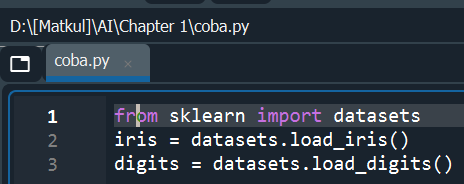
\includegraphics[width=12cm]{figures/1184023/2.PNG}
    \caption{Loading an example dataset}
    \end{figure}

\par Keterangan
    \begin{enumerate}
        \item Baris pertama: meng-import module datasets dari library sklearn.
        \item Baris kedua: iris adalah sebuah variabel dengan nilai yang memuat dataset iris dataset iris.
        \item Baris ketiga: digits adalah sebuah variabel dengan nilai yang memuat dataset digits.
    \end{enumerate}

\par Jika kode tersebut dijalankan akan menghasilkan dataset iris dan digits yang telah dimuat didalam module datasets. Berikut hasil kode yang berjalan tanpa error. Dapat dilihat pada kolom value bahwa dataset-nya telah dimuat.
    \begin{figure}[H]
    \centering
    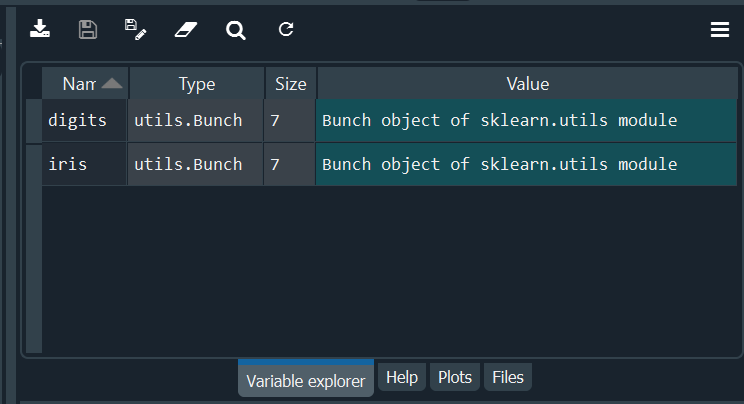
\includegraphics[width=12cm]{figures/1184023/3.PNG}
    \caption{Hasil Dataset}
    \end{figure}

\par Misalnya, untuk kumpulan data digit, Anda dapat menggunakan digits.data untuk mengakses fungsi yang dapat digunakan untuk mengklasifikasikan sampel digit:
    \begin{figure}[H]
    \centering
    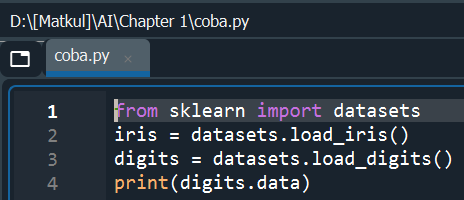
\includegraphics[width=12cm]{figures/1184023/4.PNG}
    \caption{Digits Data}
    \end{figure}

\par Disini kita menambahkan satu baris, yaitu print(digits.data) yang akan menampilkan sampel data digit. Berikut Hasilnya:
    \begin{figure}[H]
    \centering
    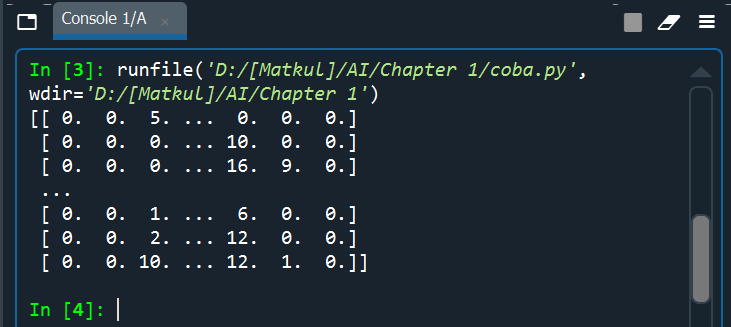
\includegraphics[width=13cm]{figures/1184023/5.PNG}
    \caption{Hasil Digits Data}
    \end{figure}
    
\par Selain digits.data, digits.target memberikan informasi dasar dari kumpulan data digit, yaitu nomor yang sesuai dengan setiap gambar digit yang ingin kita pelajari, berikut kodenya:
    \begin{figure}[H]
    \centering
    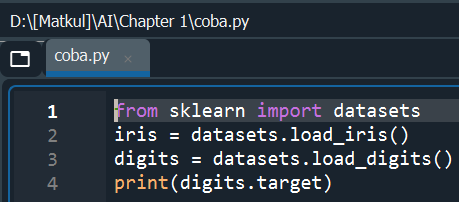
\includegraphics[width=13cm]{figures/1184023/6.PNG}
    \caption{Digits Target}
    \end{figure}

\par Seperti yang dijelaskan diatas sebelumnya digits.target akan memberikan informasi nomor setiap gambar digit yang akan dipelajari. Berikut hasilnya:
    \begin{figure}[H]
    \centering
    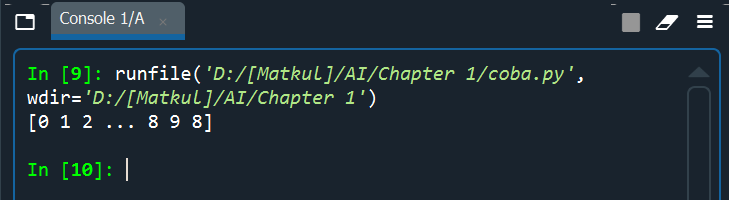
\includegraphics[width=13cm]{figures/1184023/7.PNG}
    \caption{Hasil Digits Target}
    \end{figure}

\par Meskipun data asli mungkin memiliki bentuk yang berbeda, datanya selalu berupa 2D (n-samples, n-features). Untuk digit, setiap sampel asli adalah gambar bentuk (8, 8), yang dapat diakses dengan cara berikut:
    \begin{figure}[H]
    \centering
    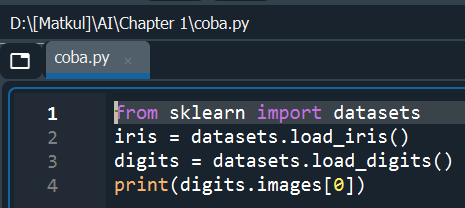
\includegraphics[width=13cm]{figures/1184023/8.PNG}
    \caption{Hasil Digits Target}
    \end{figure}

\par digits.image[0] akan menampilkan digit gambar index ke nol, yang akan menampilkan angka-angka dalam bentuk array.
    \begin{figure}[H]
    \centering
    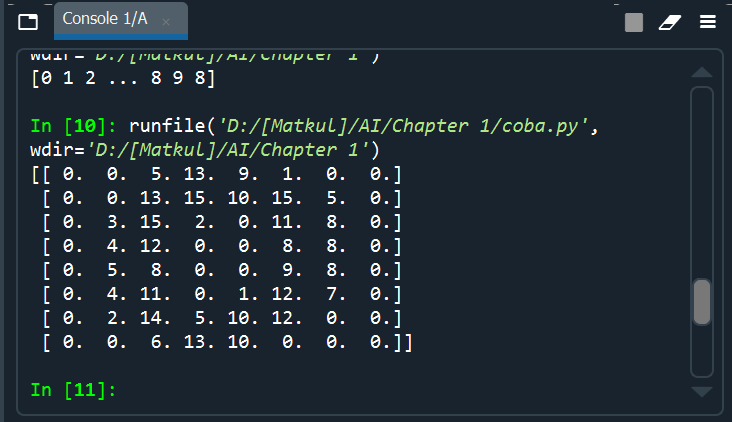
\includegraphics[width=13cm]{figures/1184023/9.PNG}
    \caption{Hasil Digits Image}
    \end{figure}

\subsection{Learning and Predicting}

\par Dalam scikit-learn, estimator yang digunakan untuk klasifikasi adalah objek Python yang mengimplementasikan metode fit (X, y) dan prediksi (T). Contoh prediktor adalah kelas sklearn.svm.SVC, yang mengimplementasikan support vector classification. Estimasi konstruktor diambil sebagai fungsi dari model parameter.

    \begin{figure}[H]
    \centering
    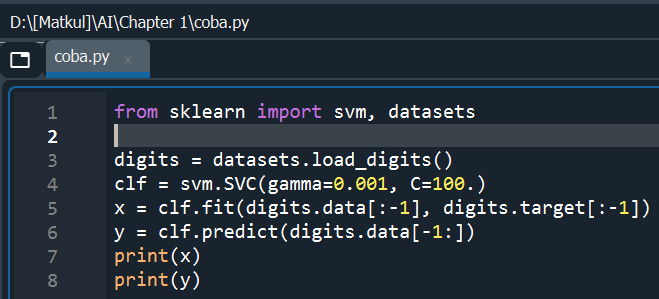
\includegraphics[width=13cm]{figures/1184023/12.PNG}
    \caption{Learning and Predicting}
    \end{figure}

\par Keterangan

    \begin{enumerate}
        \item Baris pertama mengambil module svm dan datasets dari library sklearn.
        \item Baris ketiga adalah variable dengan nama digits yang memiliki nilai untuk memuat dataset digit.
        \item Baris keempat variable clf yang memiliki value gamma=0.001 dan Classification = 100.
        \item Baris kelima variable x yang berisi clf sebagai classifier kemudian fit sebagai method yang mengambil data yang pas dari digits.data dan digits.target dengan nilai training set [:-1].
        \item Baris keenam varible y yang berisi clf sebagai classifier kemudian method predict akan memprediksi digits.data dengan nilai training set [-1:].
        \item Baris ketujuh dan kedelapan akan menampilkan hasil dari method fit dan predict.
    \end{enumerate}

\par Hasil dari method fit dan predict

    \begin{figure}[H]
    \centering
    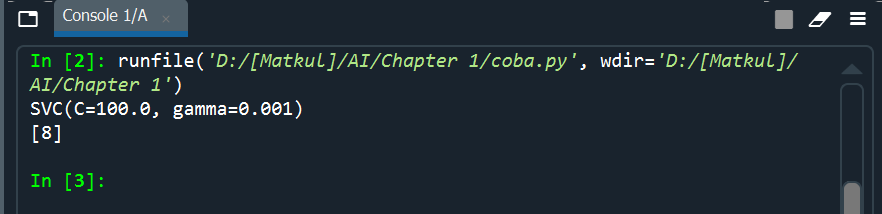
\includegraphics[width=13cm]{figures/1184023/13.PNG}
    \caption{Hasil Learning and Predicting}
    \end{figure}

\subsection{Conventions}

\subsubsection{Type Casting}

    \begin{figure}[H]
    \centering
    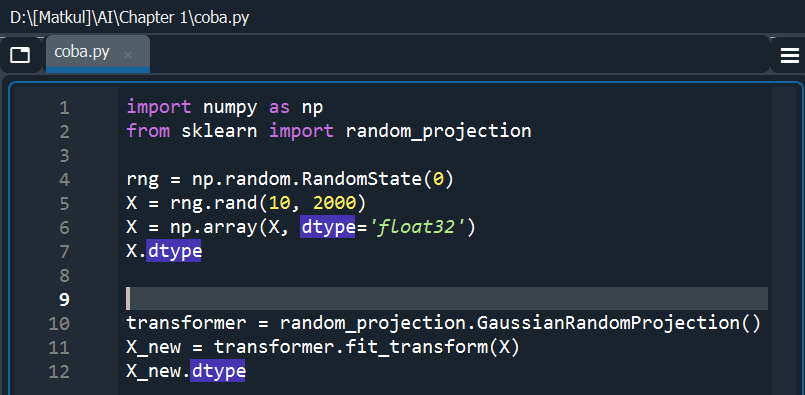
\includegraphics[width=13cm]{figures/1184023/15.PNG}
    \caption{Hasil Learning and Predicting}
    \end{figure}
    
\par Keterangan
    \begin{enumerate}
        \item Baris pertama memanggil library numpy dan dibuat dengan alias np.
        \item Baris kedua memanggil module random projection dari library sklearn.
        \item Baris keempat adalah variable rng yang mendefinisikan numpy as np, kemudian fungsi random dan attr RandomState.
        \item Baris kelima adalah variable X yang mendefinisikan variable rng, kemudian method random yang akan menentukan nilai random dari 10 - 2000.
        \item Baris keenam adalah variable X yang akan menampung nilai random sebelumnya kedalam array dengan tipe data float32.
        \item Baris ketujuh, akan mengubah tipe data nilai random float32 ke float64.
        \item Baris kesepuluh adalah sebuah variable transformer yang mendefinisikan class random projection dan memanggil fungsi GaussianRandomProjection.
        \item Baris kesebelas adalah variable X new yang akan melakukan perhitungan pada variable X.
        \item Baris keduabelas, merubah tipe data menjadi float64.
    \end{enumerate}

\par Hasil dari method X dan X new.

    \begin{figure}[H]
    \centering
    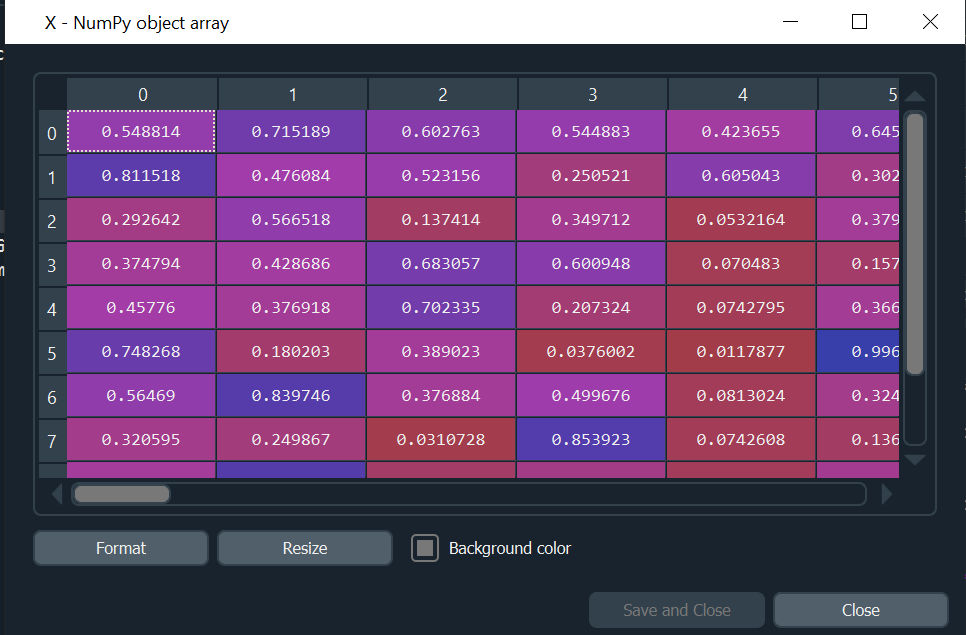
\includegraphics[width=13cm]{figures/1184023/17.PNG}
    \caption{Hasil X Numpy}
    \end{figure}
    
    \begin{figure}[H]
    \centering
    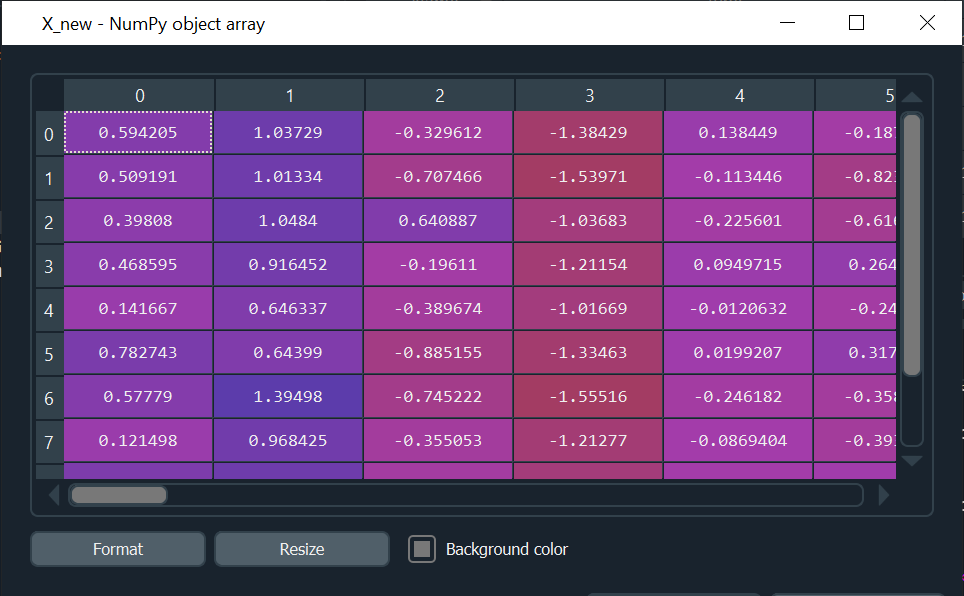
\includegraphics[width=13cm]{figures/1184023/18.PNG}
    \caption{Hasil X new Numpy}
    \end{figure}
    
\par Di sini, predict () pertama kali mengembalikan array integer, karena iris.target (array integer) digunakan dengan tepat. Prediction () kedua mengembalikan larik string karena iris.target names cocok untuk penginstalan.

    \begin{figure}[H]
    \centering
    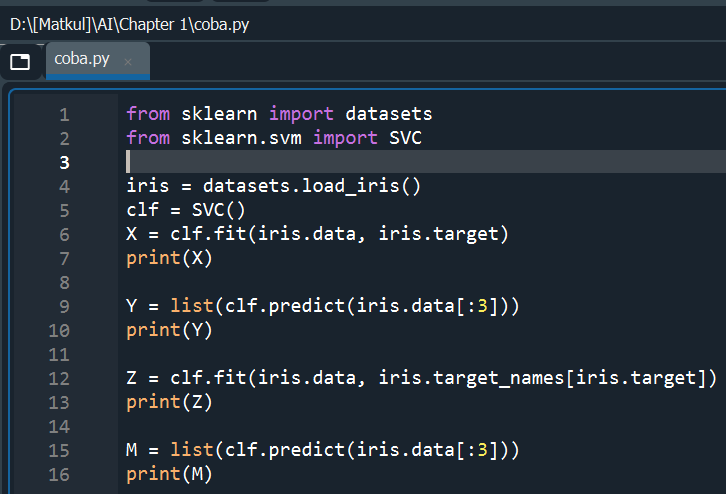
\includegraphics[width=13cm]{figures/1184023/22.PNG}
    \caption{Iris Predict}
    \end{figure}

\par Keterangan 
    \begin{enumerate}
        \item Baris pertama, memanggil module datasets dari library sklearn.
        \item Baris kedua, memanggil module SVC dari library sklearn.svm.
        \item Baris keempat, variable iris yang memuat datasets iris.
        \item Baris kelima, variable clf yang memanggil method SVC.
        \item Baris keenam, variable X yang memanggil classifier kemudian method fit yang memanggil data pas dari iris.data dan target.
        \item Baris ketujuh, menampilkan hasil variable X.
        \item Baris kesembilan, variable Y yang akan mengembalikan iris predict dalam bentuk array.
        \item Baris kesepuluh, menampilkan hasil variable Y.
        \item Baris keduabelas, memanggil classifier kemudian method fit yang memanggil data pas dari iris.names, iris.data, dan target.
        \item Baris ketigabelas, menampilkan hasil variable Z.
        \item Baris kelimabelas, variable M yang akan mengembalikan iris predict kedalam bentuk string.
        \item keenambelas, menampilkan hasil variable M.
    \end{enumerate}

\par Hasil dari iris predict.

    \begin{figure}[H]
    \centering
    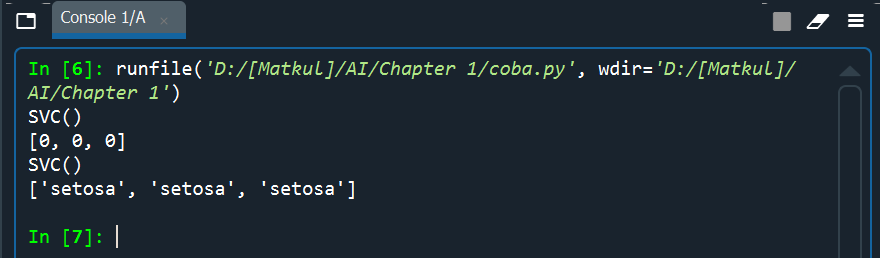
\includegraphics[width=13cm]{figures/1184023/23.PNG}
    \caption{Hasil Iris Predict}
    \end{figure}
    
\par Di sini, predict () pertama kali mengembalikan array integer, karena iris.target (array integer) digunakan dengan tepat. Prediction () kedua mengembalikan string karena iris.targetnames cocok untuk penginstalan.

\subsubsection{Refitting and updating parameters}

\par Hyperparameter dari estimator dapat diperbarui setelah dibuat dengan metode setparams (). Memanggil fit () beberapa kali akan menimpa fit () yang dipelajari sebelumnya:

    \begin{figure}[H]
    \centering
    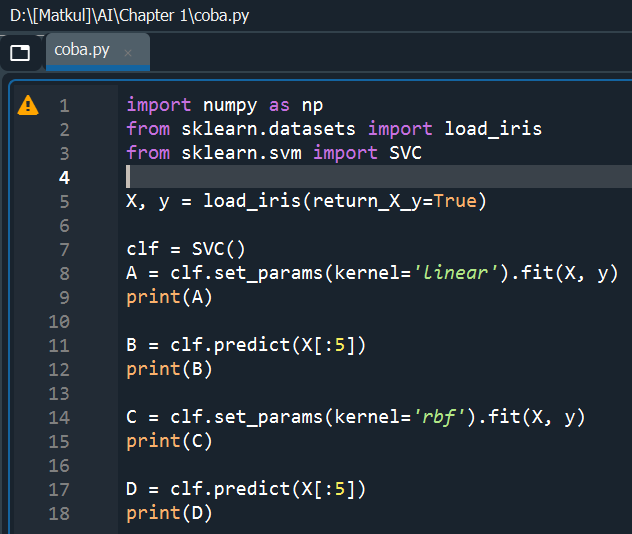
\includegraphics[width=13cm]{figures/1184023/24.PNG}
    \caption{Refitting and updating parameters}
    \end{figure}

\par Keterangan:
    \begin{enumerate}
        \item Baris pertama, memanggil library numpy dengan alias np.
        \item Baris kedua, memanggil module load iris dari library sklearn.datasets.
        \item Baris ketiga, memanggil module SVC dari library sklearn.svm.
        \item Baris kelima, mengisi variable X dan y dengan datasets iris.
        \item Baris ketujuh, mendifinisikan clf sebagai fungsi SVC.
        \item Baris kedelapan, mengubah rbf menjadi linear melalui SVC.setparams kedalam variable A.
        \item Baris kesembilan, menampilkan hasil variable A.
        \item Baris kesebelas, clf dengan method predict akan menampilkan data X dalam array sebanyak 5 data kedalam variable B.
        \item Baris keduabelas, menampilkan hasil variable B.
        \item Baris keempatbelas, mengubah linear ke rbf melalui SVC.setparams kedalam variable C.
        \item Baris kelimabelas, menampilkan hasil variable C.
        \item Baris ketujuhbelas, clf dengan method predict akan menampilkan data X dalam array sebanyak 5 data kedalam variable D.
        \item Baris kedelapanbelas, menampilkan hasil variable D.
    \end{enumerate}

\par Hasil dari Refitting and updating parameters.

    \begin{figure}[H]
    \centering
    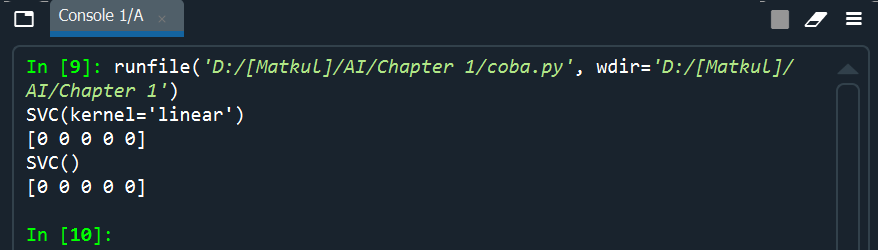
\includegraphics[width=13cm]{figures/1184023/25.PNG}
    \caption{Hasil Refitting and updating parameters}
    \end{figure}

\par Di sini, kernel default rbf pertama-tama diubah menjadi linier oleh SVC.setparams () setelah membuat estimator, dan kemudian diubah kembali ke rbf untuk mereparasi estimator dan membuat prediksi kedua.

\subsubsection{Multiclass vs. multilabel fitting}

\par Saat menggunakan multiclass classifiers, tugas learning and prediction yang dilakukan bergantung pada format data target yang sesuai, yang bergantung pada:

    \begin{figure}[H]
    \centering
    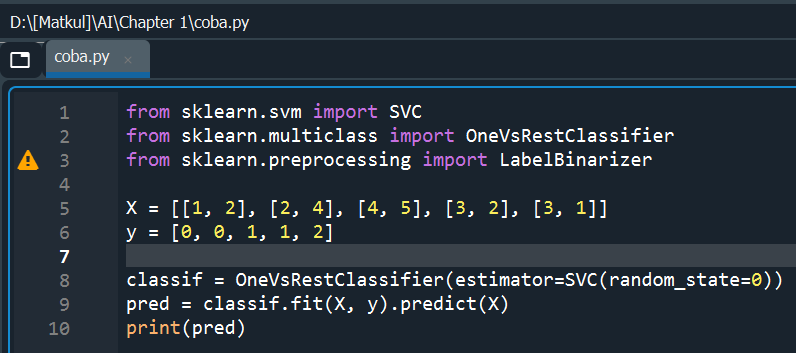
\includegraphics[width=13cm]{figures/1184023/26.PNG}
    \caption{Multiclass Predict}
    \end{figure}

\par Keterangan:
    \begin{enumerate}
        \item Baris pertama, memanggil module SVC dari library sklearn.svm.
        \item Baris kedua, memanggil module OneVsRestClassifier dari library sklearn.multiclass.
        \item Baris ketiga, memanggil module LabelBinarizer dari library sklearn.preprocessing.
        \item Baris kelima dan keenam, variable x dan y yang berisi data array.
        \item Baris kedelapan, menggunakan method OneVsRestClassifier dengan fungsi SVC sebagai estimator untuk menghasilkan data random yang didefiniskan kedalam classif.
        \item Baris kesembilan, memberikan hasil multiclass prediksi yang sesuai kedalam variable pred.
        \item Baris kesepuluh, menampilkan hasil variable pred.
    \end{enumerate}

\par Hasil dari Multiclass Predict.

    \begin{figure}[H]
    \centering
    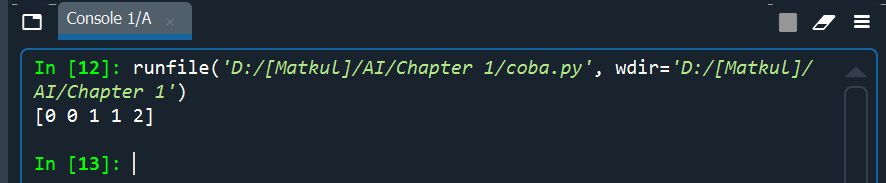
\includegraphics[width=13cm]{figures/1184023/27.PNG}
    \caption{Hasil Multiclass Predict}
    \end{figure}

\par Dalam kasus di atas, classifier cocok untuk pred label multiclass, sehingga metode predict () menyediakan prediksi multiclass yang sesuai. Dimungkinkan juga untuk menyesuaikan dengan array 2d indikator label biner:

    \begin{figure}[H]
    \centering
    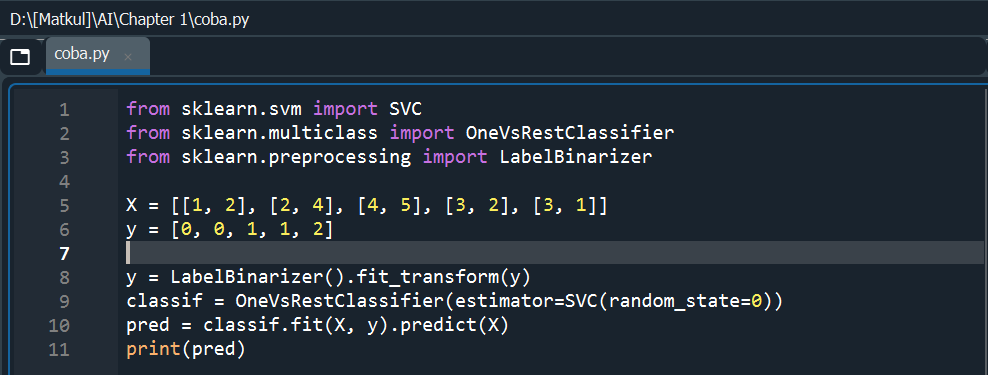
\includegraphics[width=13cm]{figures/1184023/28.PNG}
    \caption{Multiclass Predict 2}
    \end{figure}
    
\par Keterangan:
    \begin{enumerate}
        \item Baris pertama, memanggil module SVC dari library sklearn.svm.
        \item Baris kedua, memanggil module OneVsRestClassifier dari library sklearn.multiclass.
        \item Baris ketiga, memanggil module LabelBinarizer dari library sklearn.preprocessing.
        \item Baris kelima dan keenam, variable x dan y yang berisi data array.
        \item Baris kedelapan, classifier fit() merepresentasi variable y dengan LabelBinarizer.
        \item Baris kesembilan, menggunakan method OneVsRestClassifier dengan fungsi SVC sebagai estimator untuk menghasilkan data random yang didefiniskan kedalam classif.
        \item Baris kesepuluh, memberikan hasil multiclass prediksi yang sesuai kedalam variable pred.
        \item Baris kesebelas, menampilkan hasil variable pred. 
    \end{enumerate}

\par Hasil dari Multiclass Predict 2

    \begin{figure}[H]
    \centering
    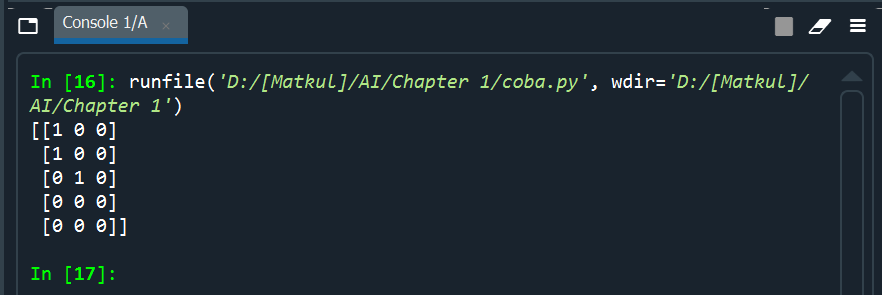
\includegraphics[width=13cm]{figures/1184023/29.PNG}
    \caption{Hasil Multiclass Predict 2}
    \end{figure}

\par Di sini, LabelBinarizer digunakan untuk menyesuaikan pengklasifikasi dengan representasi label biner pred dari y. Dalam kasus ini, predict () mengembalikan pred dalam bentuk array yang mewakili prediksi yang sesuai.

\par MultiLabel Fitting, dalam kasus ini, beberapa label ditetapkan ke classifier yang sesuai untuk setiap sampel. MultiLabelBinarizer digunakan untuk membuat binarisasi pred multilabel agar sesuai. Akibatnya, predict () mengembalikan larik pred yang berisi beberapa label yang diprediksi untuk setiap instance.

    \begin{figure}[H]
    \centering
    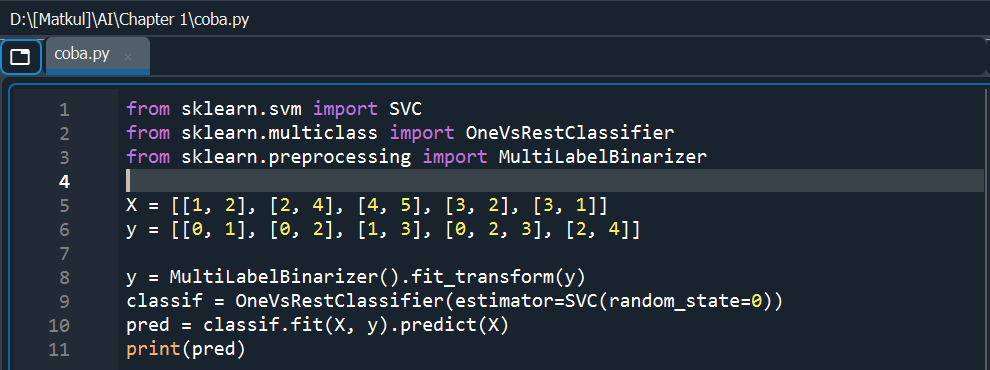
\includegraphics[width=13cm]{figures/1184023/30.PNG}
    \caption{MultiLabel Fitting}
    \end{figure}

\par Keterangan:
    \begin{enumerate}
        \item Baris pertama, memanggil module SVC dari library sklearn.svm.
        \item Baris kedua, memanggil module OneVsRestClassifier dari library sklearn.multiclass.
        \item Baris ketiga, memanggil module LabelBinarizer dari library sklearn.preprocessing.
        \item Baris kelima dan keenam, variable x dan y yang berisi data array.
        \item Baris kedelapan, classifier fit() merepresentasi variable y dengan MultiLabelBinarizer.
        \item Baris kesembilan, menggunakan method OneVsRestClassifier dengan fungsi SVC sebagai estimator untuk menghasilkan data random yang didefiniskan kedalam classif.
        \item Baris kesepuluh, memberikan hasil multiclass prediksi yang sesuai kedalam variable pred.
        \item Baris kesebelas, menampilkan hasil variable pred. 
    \end{enumerate}

\par Hasil dari Multilabel Fitting

    \begin{figure}[H]
    \centering
    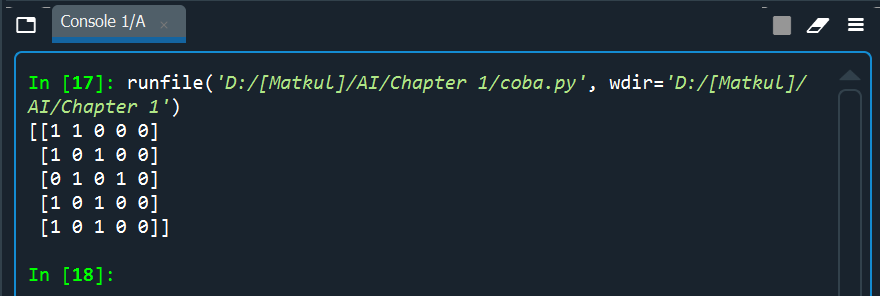
\includegraphics[width=13cm]{figures/1184023/31.PNG}
    \caption{Hasil MultiLabel Fitting}
    \end{figure}

\section{Penanganan Error}

\subsection{Error 1}

    \begin{figure}[H]
    \centering
    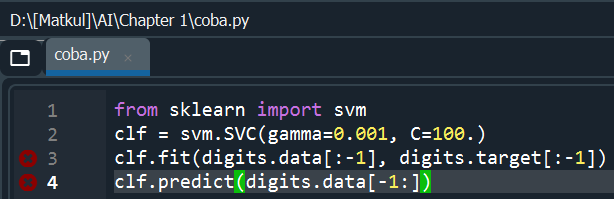
\includegraphics[width=13cm]{figures/1184023/error/1.PNG}
    \caption{Hasil MultiLabel Fitting}
    \end{figure}

\par Pada baris tiga dan empat terdapat error, yaitu sebagai berikut:

    \begin{figure}[H]
    \centering
    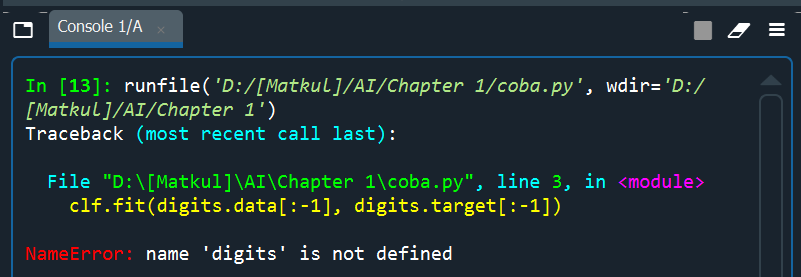
\includegraphics[width=13cm]{figures/1184023/error/2.PNG}
    \caption{Hasil MultiLabel Fitting}
    \end{figure}

\par Nama errornya adalah karena "digits" tidak terdifinisikan. Untuk penanganannya kita harus mendefinisikan digits sebagai berikut:

    \begin{figure}[H]
    \centering
    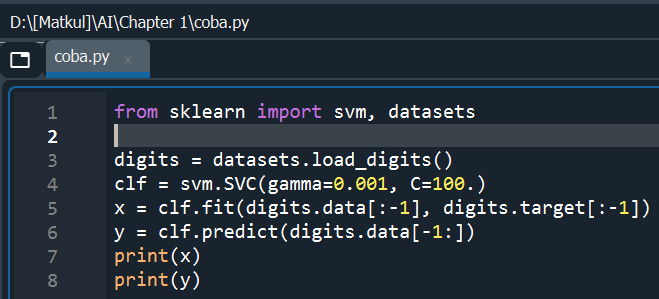
\includegraphics[width=13cm]{figures/1184023/12.PNG}
    \caption{Learning and Predicting}
    \end{figure}

\par Dapat dilihat perbedaannya pada baris pertama dan ketiga, pada baris pertama, memanggil modul datasets yang sebelumnya tidak ada dan kemudian pada baris ketiga, digits didefinisikan.
%\documentclass{homework}

\title{CHAPTER 1}
\author{1184100 MUH AMRI IRIANTO}

\begin{document}

\maketitle{SOAL CHAPTER 1 TEORI}

\section{TEORI UMUM}
\subsection{ Definisi, Sejarah dan perkembangan Kecerdasan Buatan}
\subsubsection{Definisi AI}
Kecerdasan buatan atau intelegensi artifisial dalam bahasa Inggris: Artificial Intelligence (AI) merupakan kecerdasan yang dimasukkan ke suatu sistem dan bisa diatur dalam konteks ilmiah.
Terdapat beberapa pengertian kecerdasan buatan atau artificial intelligence (AI) dalam berbagai sudut pandang.

\text Kecerdasan bauatan dalah usaha untuk memodelkan proses berfikir manusia dan mendesain mesin agar dapat menirukan perilaku manusia 
Kecerdasan bauatan juga suatu penelitian,aplikasi dan intruksi yang terkait dengan pemograman computer dalam melakukan suatu kegiatan menurut pandangan manusia

\subsubsection{Sejarah}
Dimulai pada tahun 1940 pada era computer elektronik benih-benih kecerdasan buatan ditanama kan oleh para filsuf klasik yang ingin menggabarkan proses berfikir manusia sebagai manipulasi dengan cara mekanis pada tahun 1940-an sebuah mesin yang disasarkan perangkat meginspirasi segelintir ilmuan untuk mulai serius untuk membangun sebua otak electronic.  

Istilah kecerdasan buatan pertaman kali dikemukakan pada 1956 di konfrensi Dartmouth, sejak itu kecerdasan hbuatan terus dikembangkan sebagai penelitian uuntuk teori-teori dan juga berkembangnya proinsip, Walaupun seperti itu istilah kecerdasan baru muncul pada tahun 1956 tetapi teori kecerdasan buatan sudah muncul sejak 1941

\subsubsection{Pekembangan}
Zaman computer Electronik (1941)

\text Pada tahun 1941 alat penyimpana dan pemrosesan informasi Ditemukan penemuan tersebut dinamakan Komputer electronic yang Dikembanghkan USA dan jerman. Saat itu computer melibatkan ribuan kabel untuk menjalankan suatu program.

Masa Awal Persiapan AI (1943-1956)

\text Tahun 1943 Warren McCulloch dan Walter Pitt mengemukakan tiga hal :
Pengetahuan fisiologi dasar dan fungsi sel syaraf dalam otak,analisis tengtang logika proposisi, dan teori komputasi turing mereka mamabuat midel sel sayaraf tiruan dimana setiap sel syaraf digambarkan dengan ON dan OFF menunjukkan bahawa setiap fungsi dapat dihitung  dengan suatu sel syaraf dans emua dapat di implemetasikan secara logis

\text tahun 1950, Nobert Wiener membuat penelitian mengenai prinsip-prinsip teori feedback. Contoh yang terkenal adalah thermostat. Penemuan ini juga merupakan awal dari perkembangan AI.
 
\text tahun 1956, John McCarthy meyakinkan Minsky, Claude Shannon dan Nathaniel Rochester untuk membantunya melakukan penelitian dalam bidan Otomata, Jaringan Syaraf dan pembelajaran intelijensia. Mereka mengerjakan proyek ini selama 2 bulan di Dartsmouth. Hasilnya adalah program yang mampu berpikir non-numerik dan menyelesaikan masalah pemikiran, yang dinamakan Principia Mathematica. Hal ini menjadikan McCarthy disebut sebagai bapak kecerdasan buatan.

Awal Perkembangan AI (1952-1969)

\text Pada tahun-tahun pertama perkembangannya, kecerdasan buatan mengalami banyak kesuksesan. Diawali dengan kesuksesan Newell dan Simon dengan ssebuah program yang disebut General Problem Solver.

\text Pada tahun 1958, McCarthy di MIT AI Lab Memo No.1 mendefinisikan bahasa pemrograman tingkat tinggi yaiyu LISP, yang sekarang mendominasi pembuatan program-pogram kecerdasan buatan. Kemudian, McCarthy membuat program yang dinamakan Programs with Common Sense. Di dalam program tersebut, dibuat rancangan untuk menggunakan pengetahuan dalam mencari solusi.

\text Pada tahun 1959, Nathaniel Rochester dari IBM dan mahasiswa-mahasiswanya mengeluarkan program kecerdasan buatan yaitu Geometry Theorm Prover. Program ini dapat mengeluarkan suatu teorema menggunakan aksioma-aksioma yang ada.

Sistem Berbasis Pengetahuan ( 1969 - 1979 )

\text Pengetahuan adalah kekuatan pendukung kecerdasan buatan. Hal ini dibuktikan dengan program yang dibuat oleh Ed Feingenbaum, Bruce Buchanan dan Joshua Lederberg yang membuat program untuk memecahkan masalah struktur molekul dari informasi yang didapatkan dari spectrometer massa.

Kembalinya Jaringan Syaraf Tiruan ( 1986 - Sekarang )

\text Meskipun bidang ilmu komputer menolak jaringan syaraf tiruan setelah diterbitkannya buku “Perceptrons” karangan Minsky dan Papert, para ilmuwan masih mempelajari bidang ilmu tersebut dari sudut pandang yang lain, yaitu fisika. Para ahli fisika seperti Hopfield (1982) menggunakan teknik-teknik mekanika statistika untuk menganalisia sifat-sifat penyimpanan dan optimasi pada jaringan syaraf. Para ahli psikologi, David Rumelhart dan Geoff Hinton, melanjutkan penelitian mengenai model jaringan syaraf tiruan pada memori.

\subsection{Definisi}
\subsubsection{supervise learning & unsupervise learning} supervise learning merupakan proses pegelompokan data yang telah memiliki labael dan akan dikelompokkan berdasarkan labelnya untuk mendapatkan label tertentu  untuk melakukan proses training terlebih dahulu.

unsupervised learning merupakan proses pengelompokan data yang tidak memiliki label. sehingga kita bebas meentukan jumlah kelompok data yang dibuat

\subsubsection{Klasifikasi dan Regresi}
\text klasifikasi dalah proses menemukan atau menemukan model (fungsi) yang membantu dalam memisahkan data menjadi beberapa kelas kategorikal.yang berrarti data yang dikategorikan dalam labe; yang berbeda sesuai dengan parameter

regresi adalah proses meneumkan model atau fungsi untuk emembedakan data menjadi nilai rill kotinu alih-alih menggunakna kelas secara matematis,dengan masalah regresi,sesorang berusaha menukan perkiraan fungsi dengan deviasi kesalahan minimun

\subsubsection{Dataset, Training Set dan Testing Set}
\text dataset istilah informar yang merujuk pada kumpulan data. secara umum dataset berisi lebih dari variable dan menyangkut satu topik: itu mungkin menyangkut satu sampel

Training set adalh bagian dari data set untuk memprediksi atau menjalankan fungsi dari sebuah algoritma ML. agar mesin yang kita latih mencari korelasi sendiri atau belajar denagn pola data yang diberikan

Testing set adalh bagian dataset yang kita tes untuk melihat keakuratannya atau dengan kata lain performanya



\section{IMPLEMENTASI}
untuk pertama kita bisa melakukan instalasi skit learn seperti gambar gambar dibawa melauli link
https://scikit-learn.org/stable/tutorial/basic/tutorial.html akan muncul juga tutorial mengenai penggunaan sckit learn 
\subsection{Instalasi Skit learn}
kita membuka anaconda prom terus kita bisa memasukkan 

\text conda create -n sklearn-env seperti gambar dibawah
\begin{center}
    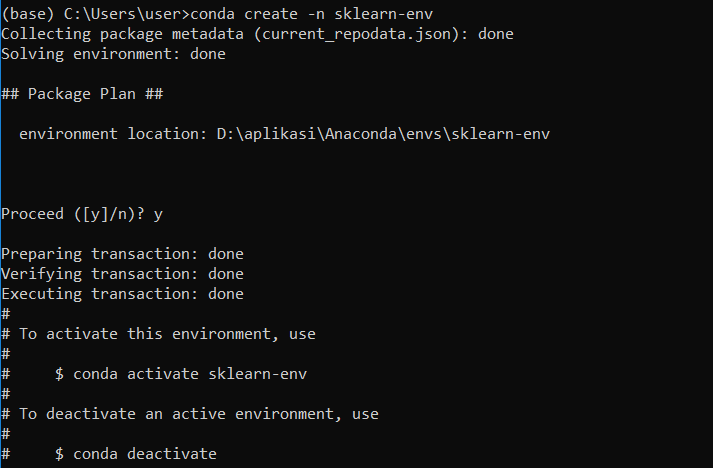
\includegraphics[width=.7\textwidth]{Figure/Instal1.PNG}
\end{center}

setelah itu kita bisa melakukan instalasi  seperti gambar dibawah untuk melihat apakah SCIKIT LEARN telah di instal
\begin{center}
    \includegraphics[width=.8\textwidth]{Figure/instal2.PNG}
\end{center}

Setelah itu,di harapkan melakuka pengecekan dengan conda seperti gambar dibawah
\begin{center}
    \includegraphics[width=.8\textwidth]{Figure/instal3.PNG}
\end{center}

\subsection{Loading an example dataset}
pada halaman ini kalan dilakukan test example data set untuk mengabil data pada scikit learn 
kita masukkan kode untuk melakukan test :

\begin{verbatim}
from sklearn import datasets
iris = datasets.load_iris()
digits = datasets.load_digits()
print(digits.data)
\end{verbatim}
maka hasilnya akan terliha seperti gambar dibawah 

\begin{center}
    \includegraphics[width=.8\textwidth]{Figure/hasil1.PNG}
\end{center}

\subsection{Learning and predicting}
pada percobaaan kali ini kita akan menggunakan learning and predicting untuk melakukan prediksi dan penggunaan leraning langsung seperti contoh dibawah

\begin{verbatim}
from sklearn import datasets 
iris = datasets.load_iris()
digits = datasets.load_digits()
from sklearn import svm
clf = svm.SVC(gamma=0.001, C=100)
clf.fit(digits.data[:-1], digits.target[:-1])
hasil = clf.predict(digits.data[-1:])
print(hasil)
\end{verbatim}
maka hasilny akan seperti gambar dibawah:
\begin{center}
    \includegraphics[width=.8\textwidth]{Figure/Hasil2.PNG}
\end{center}

\subsection{Model persistence}
pada tahap ini akan menggunakan model persintence untuk 
berikut kita bisa melihat seperti contoh dibawah untuk melakukan uji coba

\begin{verbatim}
from sklearn import svm
from sklearn import datasets
clf = svm.SVC()
X, y = datasets.load_iris(return_X_y=True)
clf.fit(X, y)

#pickle
import pickle 
s = pickle.dumps(clf)
clf2 = pickle.loads(s)
clf2.predict(X[0:1])
print(y[0])

#joblib
from joblib import dump, load
dump(clf, '1184100.joblib')
clf3 = load('1184100.joblib')
print(clf3.predict(X[0:1]))
\end{verbatim}
maka hasilnya akan seperti gambar dibawah 
\begin{center}
    \includegraphics[width=.8\textwidth]{Figure/hasil3.PNG}
\end{center}

\subsection{Conventions}
scikit-learn estimator mengikuti aturan tertentu untuk membuat perilakunya lebih prediktif,
seperti contoh dibawah:

\begin{verbatim}
import numpy as np
from sklearn import random_projection

rng = np.random.RandomState(0)
X = rng.rand(10, 2000)
X = np.array(X, dtype='float32')
X.dtype

transformer = random_projection.GaussianRandomProjection()
X_new = transformer.fit_transform(X)
X_new.dtype
print(X_new)
\end{verbatim}
maka hasilnya akan seperti gambar dibawah
\begin{center}
    \includegraphics[width=.8\textwidth]{Figure/hasil4.PNG}
\end{center}

\section{Penanganan Erorr}

\begin{enumerate}
    \item pada eororr petama ditunjukkan found input yang salah pada input found variabel
\begin{center}
    \includegraphics[width=.8\textwidth]{Figure/erorr1.PNG}
\end{center}    
    \item erorr kedua di tunjukaan pada input float sehingga varibale tidak dapat terbaca dan terjadinya errorr
\begin{center}
    \includegraphics[width=.8\textwidth]{Figure/erorr2.PNG}
\end{center} 
\end{enumerate}
\end{document}

%\section{1184077 - Alvian Daniel Sinaga}

\subsection{Teori}
\subsubsection{Definisi Kecerdasan Buatan}
\hfill\break
Kecerdasan buatan atau artificial intelligence (AI) menurut beberapa pakar adalah sebagai berikut:
\begin{enumerate}
	\item Schalkoff (1990): AI adalah bidang studi yang mencoba meniru dan menerangkan perilaku cerdas yang dilakukan oleh manusia dalam bentuk proses komputasi.
	\item Rich dan Knight (1991): AI adalah studi tentang cara membuat komputer melakukan sesuatu yang sampai saat ini orang dapat melakukannya lebih baik.
	\item Luger dan Stubblefield (1993): AI adalah cabang ilmu komputer yang berhubungan dengan otomasi perilaku yang cerdas.
\end{enumerate}

\noindent
Jadi dapat disimpulkan kecerdasan buatan atau artificial intelligence (AI) merupakan salah satu bagian ilmu komputer yang membuat mesin (komputer) dapat melakukan pekerjaan seperti dan sebaik yang dilakukan oleh manusia. Seperti yang kita tahu pada awal diciptakannya, komputer hanya difungsikan sebagai alat hitung saja. Namun seiring dengan perkembangan jaman, maka peran komputer semakin mendominasi kehidupan umat manusia. Komputer tidak lagi sekedar digunakan sebagai alat hitungn namun diharapkan untuk dapat diberdayakan untuk mengerjakan segala sesuatu yang bisa dikerjakan oleh manusia.

\subsubsection{Sejarah dan Perkembangan Kercerdasan Buatan}
\hfill\break
Istilah AI pertama kali dikemukakan pada tahun 1956 dikonferensi Darthmouth. Sejak saat itu AI terus dikembangkan sebab berbagai penelitian mengenai teori-teori dan prinsip-prinsipnya juga terus berkembang. Meskipun istilah AI baru muncul tahun 1956, tetapi teori-teori mengarah ke AI sudah muncul sejak tahun 1941. Berikut ini tahapan-tahapan sejarah perkembangan AI:
\begin{enumerate}
	\item Era Komputer Elektronik (1941)
	\hfill\break
	Pada tahun 1941 telah ditemukan alat penyimpanan dan pemrosesan informasi. Penemuan tersebut dinamakan komputer elektronik yang dikembangkan di USA dan Jerman. Komputer pertama ini memerlukan ruangan yang luas dan ruang AC yang terpisah. Saat itu komputer meibatkan konfigurasi ribuan kabel untuk menjalankan suatu program. Hal ini sangat merepotkan bagi para programmer. Pada tahun 1949, berhasil dibuat komputer yang mampu menyimpan program sehingga membuat pekerjaan untuk memasukkan program menjadi lebih mudah. Penemuan ini menjadi dasar pengembangan program yang mengarah ke AI.

	\item Masa Persiapan AI (1943–1956)
	\hfill\break
	Pada tahun 1943, Warren McCulloch dan Walter Pitts mengemukakan tiga hal: pengetahuan fisiologi dasar dan fungsi sel syaraf dalam otak, analisis formal tentang logika proporsi (propositional logic), dan teori komputasi turing. Mereka berhasil membuat suatu model syaraf tiruan (artificial neuron) di mana setiap neuron digambarkan sebagai on dan off. Mereka menunjukkan bahwa setiap fungsi dapat dihitung dengan suatu jaringan sel syaraf dan bahwa semua hubungan logis dapat diimplementasikan dengan struktur jaringan yang sederhana.
	\noindent
	Pada tahun 1950, Norbert Wiener mebuat penelitian mengenai prinsip-prinsip teori feedback. Contoh yang terkenal adalah thermostat. Penemuan ini juga merupakan awal perkembangan AI. Pada tahun 1956, John McCarthy (yang setelah lulus dari Princeton kemudian melanjutkan ke Dartmouth College) meyakinkan Minsky, Claude Shannon dan Nathaniel Rochester untuk membantunya melakukan penelitian dalam bidang Automata, jaringan sel syaraf dan pembelajaran intelejensia. Mereka mengerjakan proyek ini selama dua bulan di Dartmouth. Hasilnya adalah program yang mampu ber-pikir non-numerik dan menyelesaikan masalah pemikiran, yang dinamakan Principia Mathematica. Hal ini menjadikan McCarthy disebut sebagai Father of AI (Bapak AI).

	\item Awal Perkembangan AI (1952–1969)
	\hfill\break
	Pada tahun-tahun pertama pengembangannya, AI mengalami banyak kesuksesan. Diawali dengan kesuksesan Newell dan Simon dengan sebuah program yang disebut General Problem Solver. Program ini dirancang untuk memulai penyelesaian masalah secara manusiawi. Pada tahun 1958, McCarthy di MTT Lab Memo No. 1 mendefinisikan bahasa pemrograman tingkat tinggi yaitu LISP, yang sekarang mendominasi pembuatan program-program AI. Kemudian, McCarthy membuat program yang dinamakan Programs With Common Sense. Di dalam program tersebut, dibuat rancangan untuk menggunakan pengetahuan dalam mencari solusi. Pada tahun 1959, Nathaniel Rochester dari IBM dan mahasiswa-mahasiswanya mengeluarkan program AI Geometry Theorm Prover. Program ini dapat membuktikan suatu teorema menggunakan axioma-axioma yang ada. Pada tahun 1963, program yang dibuat James Slagle mampu menyelesaikan masalah integral tertutup untuk mata kuliah kalkulus. Pada tahun 1968, program analogi buatan Tom Evan menyelesaikan masalah analogi geometris yang ada pada tes IQ.

	\item Perkembangan AI Melambat (1966–1974)
	\hfill\break
	Prediksi Herbert Simon pada tahun 1957 yang menyatakan bahwa AI akan menjadi ilmu pengetahuan yang akan berkembang dengan pesat ternyata meleset. Pada 10 tahun kemudian, perkembangan AI melambat. Hal ini disebabkan adanya 3 kesulitan utama yang dihadapi AI, yaitu:
	\begin{enumerate}
		\item Masalah pertama: program-program AI yang bermunculan hanya mangandung sedikit atau bahkan tidak mengandung sama sekali pengetahuan (knowledge) pada subjeknya. Program-program AI berhasil hanya karena manipulasi sintetis yang sederhana. Sebagai contoh adalah Weizenbaum’s ELIZA program (1965) yang dapat melakukan percakapan serius pada berbagai topik, sebenarnya hanyalah peminjaman dan manipulasi kalimat-kalimat yang diketikkan oleh manusia.
		\item Masalah kedua: banyak masalah yang harus diselesaikan oleh AI. Karena terlalu banyaknya masalah yang berkaitan, maka tidak jarang banyak terjadi kegagalan pada pembuatan program AI.
		\item Masalah ketiga: ada beberapa batasan pada struktur dasar yang digunakan untuk menghasilkan perilaku intelejensia. Sebagai contoh adalah pada tahun 1969 buku Minsky dan Papert Perceptrons membuktikan bahwa program-program perceptrons dapat mempelajari segala sesuatu, tetapi program-program tersebut hanya mempresentasikan sejumlah kecil saja. Sebagai contoh dua masukan perceptrons yang berbeda tidak dapat dilatihkan untuk mengenali kedua masukan yang berbeda tersebut.
	\end{enumerate}

	\item Sistem Berbasis Pengetahuan (1969–1979)
	\hfill\break
	Pengetahuan adalah kekuatan pendukung AI. Hal ini dibuktiikan dengan program yang dibuat oleh Ed Feigenbaum,Bruce Buchanan dan Joshua Lederberg yang membuat program untuk memecahkan masalah struktur molekul dari informasi yang didapatkan dari spectometer massa. Program ini dinamakan Dendral programs yang berfokus pada segi pengetahuan kimia. Dari segi diagnosis media juga sudah ada yang menemukannya, yaitu Saul Amarel dalam proyek computer in biomedicine. Proyek ini diawali dari keinginan untuk mendapatkan diagnosa penyakit berdasarkan pengetahuan yang ada pada mekanisme penyebab proses penyakit.

	\item AI Menjadi Sebuah Industri (1980–1988)
	\hfill\break
	Industrialisasi AI diawali dengan ditemukannya expert system (sistem pakar) yang dinamakan R1 yang mampu mengkonfigurasi sistem-sistem komputer baru. Program tersebut mulai dioperasikan di Digital Equipment Corporation(DEC), McDermott, pada tahun 1982. Pada tahun 1986, program ini telah berhasil menghemat US\$40 juta per tahun. Pada tahun 1988, kelompok AI di DEC menjalankan 40 sistem pakar. Hampir semua perusahaan besar di USA mempunyai divisi AI sendiri yang menggunakan ataupun mempelajari sistem pakar. Booming industri AI ini juga melibatkan perusahaan-perusahaan besar seperti Carnegie Group, Inference, Intellicorp, dan Technoledge yang menawarkan software tools untuk membangun sistem pakar. Perusahaan hardware seperti LISP dan Machines Inc., Texas Instruments, Symbolics, dan Xerox juga turut berperan dalam membangun workstation yang dioptimasi untuk pembangunan program LISP. Sehingga, perusahaan yang sejak tahun 1982 hanya menghasilkan beberapa juta US dolar per tahun meningkat menjadi 2 milyar US dolar per tahun pada tahun 1988.

	\item Kembalinya Jaringan Syaraf Tiruan (1986–Sekarang)
	\hfill\break
	Meskipun bidang ilmu komputer menolak jaringan syaraf tiruan setelah diterbitkannya buku "perceptrons" karangan Minsky dan Papert, tetapi para ilmuan masih mempelajari bidang ilmu tersebut dari sudut pandang yang lain yaitu fisika. Para ahli seperti Hopfield (1982) menggunakan teknik-teknik mekanika statistika untuk menganalisa sifat-sifat penyimpanan dan optimasi pada jaringan syaraf. Para ahli psikollogi, David Rumelhart dan Geoff Hinton, melanjutkan penelitian mengenai model syaraf pada memori. Pada tahun 1985-an sedikitnya empat kelompok riset menemukan kembali algoritma belajar propagasi balik (Back-Propagation Learning). Algoritma ini berhasil diimplementasikan kedalam bidang ilmu komputer dan psikologi.

\end{enumerate}

\subsubsection{Supervised Learning}
\hfill\break
Supervised Learning adalah pembelajaran yang memiliki label di tiap datanya. Label maksudnya adalah tag dari data yang ditambahkan dalam machine learning model. Contohnya gambar kucing di tag "kucing" di tiap masing masing image kucing dan gambar anjing di tag "anjing" di tiap masing gambar anjing. Machine learning kategori dapat berupa clasification ("anjing", "kucing", "beruang", dsb) dan regression ( berat badan, tinggi badan dsb). Supervised learning banyak digunakan dalam memprediksi pola dimana pola tersebut sudah ada contoh data yang lengkap, jadi pola yang terbentuk adalah hasil pembelajaran data lengkap tersebut. Tentunya jika kita memasukan data baru, setelah kita melakukan ETL (Extract Transform Load) maka kita mendapat info feature feature dari sample baru tersebut. Kemudian dari feature feature tersebut di compare dengan pattern clasification dari model yang didapat dari labeled data. Setiap label akan dicompare sampai selesai, dan yang memiliki percentage lebih banyak akan diambil sebagai prediksi akhir.

\begin{figure}[H]
	\includegraphics[width=1\textwidth]{figures/1184077/chapter1/supervisedlearning.jpeg}
	\centering
	\caption{Supervised Learning.}
\end{figure}
\noindent
Contoh algoritma yang digunakan pada supervised learning meliputi :
\begin{enumerate}
	\item Clasification (Categorical) and Regression (Numerical)
    \item Logistic Regression
    \item Model Ensemble
	\item Time series
\end{enumerate}

\subsubsection{Klasifikasi}
\hfill\break
Classification adalah tindakan untuk memberikan kelompok pada setiap keadaan. Setiap keadaan berisi sekelompok atribut, salah satunya adalah class attribute. Metode ini butuh untuk menemukan sebuah model yang dapat menjelaskan class attribute itu sebagai fungsi dari input attribute.

\noindent
Class adalah attribute CollegePlans yang berisi dua pernyataan, Yes dan No, perhatikan ini.
\noindent
Sebuah Classification Model akan menggunakan atribut lain dari kasus tersebut (input attribut; yaitu kolom IQ, Gender, ParentIncome, dan ParentEncouragement) untuk dapat menentukan pola (pattern) class (Output Attribute; yaitu Kolom CollegePlans yang berisi Yes atau No).
\noindent
Algoritma Data Mining yang membutuhkan variabel target untuk belajar (sampai mendapatkan rule / pola yang berlaku pada data tersebut) kita standarkan dengan sebuthan dengan Supervised Algorithm.
\noindent
Nah, yang termasuk kepada Classification Algorithm adalah Decision Trees, Neural Network dan Naives Bayes.
\subsubsection{Regresi}
\hfill\break
Metode Regression mirip dengan metode Classification, yang membedakannya adalah metode regression tidak bisa mencari pola yang dijabarkan sebagai class (kelas).
\noindent
Metoda regression bertujuan untuk mecari pola dan menentukan sebuah nilai numerik.
\noindent
Sebuah Teknik Linear Line-fitting sederhana adalah sebuah contoh dari Regression, dimana hasilnya adalah sebuah fungsi untuk menentukan hasil yang berdasarkan nilai dari input.
\noindent
Bentuk yang lebih canggih dari regression sudah mendukung input berupa kategori, jadi tidak hanya input berupa numerik. Teknik paling popular yang digunakan untuk regression adalah linear regression dan logistic regression. Teknik lain yang didukung oleh SQL Server Data mining adalah Regression Trees (bagian dari dari algoritma Microsoft Decission Trees) dan Neural Network.
\noindent
Regression digunakan untuk memecahkan banyak problem bisnis – contohnya untuk memperkirakan metode distribusi, kapasitas distribusi, musim dan untuk memperkirakan kecepatan angin berdasarkan temperatur, tekanan udara, dan kelembaban.
\subsubsection{Unsupervised Learning}
\hfill\break
Unsupervised learning memiliki keunggulan dari supervised learning. Jika supervised learning memiliki label sebagai dasar prediksi baik serta membuat clasification dan regression algorithm memungkinkan. Tetapi dalam realitanya, data real itu banyak yang tidak memiliki label. Label kebanyakan jika data sudah masuk ke ERP apapun bentuk ERPnya dan bagaimana kalo datanya berupa natural input seperti suara, gambar, dan video. Unsupervised learning tidak menggunakan label dalam memprediksi target feautures / variable. Melainkan menggunakan ke samaan dari attribut attribut yang dimiliki. Jika attribut dan sifat-sifat dari data data feature yang diekstrak memiliki kemirip miripan, maka akan dikelompok kelompokan (clustering). Sehingga hal ini akan menimbulkan kelompok kelompok (cluster). Jumlah cluster bisa unlimited. Dari kelompok kelompok itu model melabelkan, dan jika data baru mau di prediksi, maka akan dicocok kan dengan kelompok yang mirip mirip featurenya.
\begin{figure}[H]
	\includegraphics[width=1\textwidth]{figures/1184077/chapter1/unsupervisedlearning.jpg}
	\centering
	\caption{Unsupervised Learning.}
\end{figure}
\noindent
Tetapi unsupervise learning tidak memiliki outcome yang spesifik layaknya di supervise learning, hal ini dikarenakan tidak adanya ground truth / label dasar. Walaupun begitu, unsupervised learning masih dapat memprediksi dari ketidakadaan label dari kemiripan attribute yang dimilik data.
\noindent
Algoritma yang digunakan di unsupervised learning :
\begin{enumerate}
	\item Clustering
    \item Anomaly Detection
    \item Training Model
    \item Association Discovery
\end{enumerate}
\subsubsection{Data Set}
\hfill\break
Dataset adalah objek yang merepresentasikan data dan relasinya di memory. Strukturnya mirip dengan data di database. Dataset berisi koleksi dari datatable dan data relation.
\subsubsection{Training Set}
\hfill\break
Training set adalah bagian dataset yang kita latih untuk membuat prediksi atau menjalankan fungsi dari sebuah algoritma ML lainnya sesuai tujuannya masing-masing. Kita memberikan petunjuk melalui algoritma agar mesin yang kita latih bisa mencari korelasinya sendiri. 
\subsubsection{Testing Set}
\hfill\break
Test set adalah bagian dataset yang kita tes untuk melihat keakuratannya, atau dengan kata lain melihat performanya.


\subsection{Praktek}
\begin{enumerate}
	\item Instalasi  library  scikit  dari  anaconda,  mencoba  kompilasi  dan  uji  coba  ambil contoh kode dan lihat variabel explorer.
	
	\textbf{Instalasi Library Scikit-Learn melalui CMD }
	\begin{enumerate}
		\item Pertama masuk ke command prompt di menu start.
		\begin{figure}[H]
			\includegraphics[width=1\textwidth]{figures/1184077/chapter1/praktek/1.PNG}
			\centering
			\caption{Instalasi Library Scikit-Learn.}
		\end{figure}
		\item Selanjutnya ketik "conda activate base" untuk masuk base anaconda.
		\item Kemudian ketik conda install scikit-learn.
		\item Lalu apabila sudah done , artinya library scikit sudah kita install
	\end{enumerate}

	\textbf{Mencoba Menggunakan Library scikit-Learn}
	\begin{enumerate}
		\item Pertama jalankan aplikasi Spyder.
		\item Kemudian buat file baru, lalu tambahkan kode berikut.
		\lstinputlisting[language=Python]{src/1184077/chapter1/contoh.py}
		\item Simpan dan jalankan.
		\item Hasil dari variabel explorernya sebagai berikut.
		\begin{figure}[H]
			\includegraphics[width=1\textwidth]{figures/1184077/chapter1/praktek/contoh.PNG}
			\centering
			\caption{Variabel Explorer Library Scikit-Learn.}
		\end{figure}
	\end{enumerate}
	
	\item Mencoba Loading an example dataset, menjelaskan maksud dari tulisan terse-but dan mengartikan per baris.
	\lstinputlisting[firstline=3,lastline=7]{src/1184077/chapter1/Tugas1.py}
	
	Hasilnya akan seperti ini.
	\begin{figure}[H]
		\includegraphics[width=7cm]{figures/1184077/chapter1/praktek/hasil1.PNG}
		\centering
		\caption{Hasil Loading an Example Dataset.}
	\end{figure}

	\item Mencoba  Learning  and  predicting,  menjelaskan  maksud  dari  tulisan  tersebut dan mengartikan per baris.
	\lstinputlisting[firstline=11,lastline=14]{src/1184077/chapter1/Tugas1.py}
	
	Hasilnya akan seperti ini.
	\begin{figure}[H]
		\includegraphics[width=7cm]{figures/1184077/chapter1/praktek/hasil2.PNG}
		\centering
		\caption{Hasil Learning and Predicting.}
	\end{figure}

	\item Mencoba Model persistence, menjelaskan maksud dari tulisan tersebut dan mengartikan per baris.
	\lstinputlisting[firstline=18,lastline=34]{src/1184077/chapter1/Tugas1.py}
	
	Hasilnya akan seperti ini.
	\begin{figure}[H]
		\includegraphics[width=8cm]{figures/1184077/chapter1/praktek/hasil3.PNG}
		\centering
		\caption{Hasil Model Persistence.}
	\end{figure}

	\item Mencoba Conventions, menjelaskan maksud dari tulisan tersebut dan mengartikan per baris.
	\lstinputlisting[firstline=35,lastline=49]{src/1184077/chapter1/Tugas1.py}
	
	Hasilnya akan seperti ini.
	\begin{figure}[H]
		\includegraphics[width=10cm]{figures/1184077/chapter1/praktek/hasil4.PNG}
		\centering
		\caption{Hasil Conventions.}
	\end{figure}

\end{enumerate}

\subsection{Penanganan Error}
\begin{enumerate}
	\item Screenshoot error yang terjadi pada saat melakukan running syntax pada saat melakukan praktikum ini.
	\begin{itemize}
		\item Name Error dapat terjadi apabila terdapat kesalahan penulisan syntax, yang meliputi nama library, function etc.
		\hfill\break
		\begin{figure}[H]
			\includegraphics[width=10cm, height=3cm\textwidth]{figures/1184077/chapter1/error/error1.PNG}
			\centering
			\caption{Name Error.}
		\end{figure} \\ 

		\item Import Error
		\hfill\break
		\begin{figure}[H]
			\includegraphics[width=1\textwidth]{figures/1184077/chapter1/error/error2.PNG}
			\centering
			\caption{Import Error.}
		\end{figure}
		\item Syntax Error
		\hfill\break
		\begin{figure}[H]
			\includegraphics[width=1\textwidth]{figures/1184077/chapter1/error/error3.PNG}
			\centering
			\caption{Syntax Error.}
		\end{figure}
	\end{itemize}
	\item Tuliskan kode eror dan jenis errornya.
	\begin{itemize}
		\item Name Error
		\hfill\break
		Name Error adalah exception yang terjadi saat syntax melakukan eksekusi terhadap local name atau global name yang tidak terdefinisi.
		\item Import Error
		\hfill\break
		Import Error adalah exception yang terjadi saat syntax melakukan import terhadap library yang tidak terdefinisi.
		\item Syntax Error
		\hfill\break
		Syntax Error adalah exception yang terjadi saat ada kesalahan dalam mengetikkan syntax.
	\end{itemize}
	\item Solusi pemecahan masalah error tersebut.
	\begin{itemize}
		\item Name Error
		\hfill\break
		Solusinya adalah memastikan variabel atau function yang dipanggil ada atau tidak salah ketik.
		\item Import Error
		\hfill\break
		Solusinya adalah memastikan library yang dipanggil ada atau tidak salah ketik.
		\item Syntax Error
		\hfill\break
		Solusinya adalah memastikan syntax yang diketik tidak salah ketik.
	\end{itemize}
\end{enumerate}

\subsection{Bukti Tidak Plagiat}
\begin{figure}[H]
	\includegraphics[width=1\textwidth]{figures/1184077/chapter1/plagiat.PNG}
	\centering
	\caption{Bukti Tidak Plagiat.}
\end{figure}
%\section{Yusuf Jordan El Anwar - 1184026}
\subsection{Teori}
\begin{enumerate}

	\item Definisi Kecerdasan Buatan
	\hfill\break
	Kecerdasan buatan atau artificial intelligence (AI) adalah sebuah teknologi buatan manusia yang di modelkan ke dalam sebuah mesin dan mesin di tersebut di program supaya dapat berpikir seperti manusia sehingga dapat bekerja layaknya manusia dan berpikir seperti manusia sehingga dapat memudahkan pekerjaan manusia.

    AI ini merupakan sebuah mesin dan tidak memiliki kecerdasan sehingga untuk itu kita perlu menambahkan data dan pengalaman kepada mesin tersebut supaya mesin tersebut dapat memiliki kecerdasan. Point penting didalam ai adalah learning, reasoning, dan self correcting.
	\item Sejarah dan Perkembangan
	\hfill\break
    AI tersusun dari 2 kata yaitu artificial intelligence. Intelligence sendiri berasal dari kata Yunani “intelligo” yang memiliki arti “saya paham”. Dan intelligence memiliki arti dasar kemampuan untuk memahami kemudian pemahaman tersebut di lakukan.
    Sejarah kecerdasan buatan sudah ada pada zaman kuno namun dikenal sebagai cerita tentang mahkluk buatan yang diberkahi oleh para pengrajin. Sehingga akhirnya sebuah karya memuncak saat penemuan komputer digital yang diprogram pada tahun 1940-an.
    Pada tahun 1965 istilah kecerdasan buatan pertama kali di perkenalkan di konferensi darthmouth dan dikembangkan hingga sekarang
    Sekitar akhir tahun 1955, Newell dan Simon mengembangkan program ai pertama yang di namakan The Logic Theorist. Program ini memiliki dampak yang besar dan menjadi batu loncatan penting dalam sejarah perkembangan  AI. Satu tahun setelahnya yaitu pada tahun 1956 John McCarthy guru dari Massacuhetts Institute of Technology dianggap sebagai bapak AI karena menyelenggarakan konferensi “The Dartmouth summer research project on artificial intelligence” untuk menarik para ahli komputer bertemu.  Di Konferensi Dartmouth itu akhirnya mempertemukan cikal bakal para pendiri dalam AI yang akhirnya  meletakkan dasar bagi generasi di masa depan untuk  mengembangkan dan melakukan penelitian pada bidang AI. Sekitar  tahun 1960 hingga 1970 muncul berbagai komunitas yang berdiskusi bagaimana komputer dapat meniru sedetail mungkin pada kemampuan otak manusia sehingga memunculkan isitilah “classical AI”. Mulai tahun 1980, computer semakin mudah diperoleh dengan harga yang lebih murah, sehingga menjadikan berbagai riset di bidang kecerdasan buatan semakin berkembang pesat pada berbagai universitas.
    Perkembangan awal AI ( 1952 - 1969 )
    Perkembangan awal ai di mulai ketika Newell dan Simon membuat sebuah program yang dikenal sebagai General Problem Solver yang dirancang untuk mengembangkan sebuah penyelesaian masalah secara manusiawi yang akhirnya berakhir dengan kesuksesan.
    Di lanjutkan oleh James Slagel pada tahun 1963 yaitu membuat sebuah program untuk menyelesaikan masalah integral tertutup untuk membantu pada bidang matakuliah kalkulus.
    Dan terakhir pembuatan program untuk memberikan analalogi penyelesaian masalah analogi geometris pada tes iq yang di ciptakan oleh Tom Evans.
    Perkembangan Kecerdasan Buatan ( 1966  –  1974 )
    Pada fase ini perkembangan kecerdasan mulai melambat karena beberapa factor. Yaitu : 
    Pertama, Program yang berhasil  hanya diciptakan karena manipulasi program sebelumnya.
    Kedua, Banyak masalah masalah kompleksyang harus di selesaikan kecerdasan buatan.
    Ketiga, Mulai adanya beberapa Batasan pada struktur dasar sehingga menyulitkan untuk menghasilkan perilaku intelligence.
    Sistem berbasis Pengetahuan ( 1969 - 1979 )
     Ed Feingenbaum, Bruce Buchanan dan Joshua Lederberg berhasil membuat sebuah program untuk memecahkan masalah struktur molekul dalam bidang kimia
    Industri Kecerdasan Buatan ( 1980 – 1988 )
    Kecerdasan buatan mulai merambah dunia industry ketika ditemukannya system pakar yang bernama R1 yang dapat mengkonfigurasi system – system pada computer baru.
    Jaringan Syaraf Tiruan ( 1986 – Sekarang )
    Sekelompok periset menemukan algoritma yang di implementasikan pada bidang ilmu computer dan psikologi .  algoritma ini di namakan algoritma belajar propagasi balik.
\begin{itemize}
		\item Supervised dan Unsupervised Learning
		\hfill\break
	Supervised learning adalah metode pendekatan pengelompokan data atau variable yang sudah di targetkan dan mengelompokan data tersebut ke dalam data yang telah ada. Sedangakn Unsupervised learning adalah metode pendekatan yang tidak memliki data sehingga data yang ada harus di pilah menjadi beberapa kategori atau bagian.
		\item Klasifikasi dan Regresi
		\hfill\break
		Klasifikasi adalah sebuah metode pengelompokan data berdasarkan standard yang telah ada. Sedangkan regresi adalah sebuah metode analisis statistik untuk melihat bagaimana pengaruh suatu variable.
		\item Definisi Dataset, Trainig Set dan Testing Set
		\hfill\break
        Dataset adalah objek yang berfungsi untuk mempresentasikan data atau relasi di dalam memori.
        Training set adalah bagian dataset yang dapat membuat memprediksi atau algoritma berdasarkan tujuan masing masing
        Testing Set adalah bagian dari dataset dilakukan tes untuk melihat seberapa akurat dan ketepatan datanya.  
	\end{itemize}
\end{enumerate}
\subsection{Praktek}
\begin{enumerate}
\item Instalasi Library scikit dari Anaconda, mencoba kompilasi dan uji coba ambil contoh kode dan lihat variabel explorer
	\hfill\break
	\begin{figure}[h]
		\includegraphics[width=10cm]{figures/1184026/chapter1/Capture.PNG}
		\centering
		\caption{Instalasi Library Scikit Learn}
	\end{figure}
	\begin{figure}[h]
		\includegraphics[width=10cm]{figures/1184026/chapter1/variabel eksplore.PNG}
		\centering
		\caption{Isi Variabel Explorer}
	\end{figure}
	\item Uji coba loading an example dataset
	\hfill\break
\lstinputlisting[firstline=1, lastline=4]{src/1184026/chapter1/belajar.py}
\item Uji coba Learning dan predicting
	\hfill\break
	\lstinputlisting[firstline=8, lastline=15]{src/1184026/chapter1/contoh2.py}
\item Uji coba Model Persistence
	\hfill\break
	\lstinputlisting[firstline=8, lastline=32]{src/1184026/chapter1/contoh3.py}
	\item Uji coba Conventions
	\hfill\break
	\lstinputlisting[firstline=8, lastline=19]{src/1184026/chapter1/contoh4.py}
\end{enumerate}
\begin{enumerate}
	\item ScreenShoot Error
	\begin{figure}[h]
		\includegraphics[width=10cm]{figures/1184026/chapter1/eror1.PNG}
		\centering
		\caption{Name Error}
	\end{figure}
	\item Tuliskan Kode Error dan Jenis Error
	\hfill\break
	Name 'datasets' is not defined
\hfill\break
	\item Cara Penangan Error
\hfill\break Tambahkan variabel datasets agar kode program dapat terbaca
	\end{enumerate}

%\begin{document}

\maketitle

\section{1184095 Dian Markuci}
\subsection{Teori}
	\subsubsection{Sejarah Perkembangan dan Definisi Artificial Intelligence}      
	
	\begin{enumerate}
	    \item  Kecerdasan Buatan atau \textit{Artificial Intelligence} (AI) merupakan perkembangan teknologi yang menarik perhatian. AI meniru kecerdasan makhluk hidup ataupun benda mati untuk menyelesaikan persoalan. dari drama korea Are you human too disana menceritakan sebuah robot AI seperti manusia, dengan kehadiran film fiksi ilmiah yang berhubungan dengan AI membuat semakin banyak ketertarikan dibidang AI. Sekarang saja di Jepang sudah dibuat robot AI yang menyerupai manusia. 
	    
	    \item  Tahun 1956 merupakan kali pertama muncul istilah Artificial Intellegent. Kemudian tahun 1950-an dilakukan tahap riset awal proyek AI yang bertujuan mengeksplorasi topik penyelesaian persoalan dan metode simbolik. Berikutnya di Amerika Serikat tahun 1960-an Departemen Pertahanan ingin melatih serta melakukan pengembangan komputer agar memiliki nalar yang menyerupai manusia secara dasar.  keberhasilan menyelesaikan studi kasus tentang pemetaan jalan merupakan proyek DARPA (Defence Advanced Research Project Agency) ditahun 1970 -an. Pada abad ke – 21 tepatnya tahun 2003, DARPA menciptakan asisten pribadi cerdas.  AI menerapkan algoritma dari pembelajaran secara mendalam atau deep learning. Kini ada kelebihan AI dibanding manusia, Pada tahun 2016 AI yang dipunyai AlphaGo yaitu menariknya manusia hanya bisa bermain satu kali dalam satu waktu. dengan bukti AlphaGo bisa bermain dengan juara dunia Go dan bisa memenangkan permainannya.
	    
	\end{enumerate}
    
    

    \subsubsection{Supervised learning, Klasifikasi, Regresi dan unsupervised learning. Data set, Training set dan Testing set}
    
    \begin{enumerate}
    
    \item Supervised learning adalah pembelajaran yang disertai pengawas atau dapat di sebut ada supervisornya. Pengawas disini memiliki arti label yang ada di setiap data. Kemudian label tersebut dimaksudkan sebagai tag dari data yang ditambah ke dalam model pembelajaran mesin atau sering disebut machine learning model. Bisa di beri gambaran misal seperti gambar pepaya di tag “pepaya” di masing masing gambar pepaya dan gambar paprika di tag “paprika” di masing masing gambar paprika. Machine learning kategori dapat berupa clasification (“pepaya”, “paprika”, dsb) dan regression ( tinggi badan, berat badan, dsb). 

    \item Klasifikasi dan Regresi
Cara kerja supervised learning dalam ilustrasi ini dibagi menjadi dua yaitu klasifikasi dan regresi. Mesin dapat mengelompokan data sesuai klasifikasinya. Kemudian regresi mampu mengidentifikasi data nyata berupa angka seperti tinggi, berat, ataupun dollar. Dalam dunia data science supervised learning merupakan algoritma yang lebih sering digunakan dibandingkan dengan unsupervised learning. Di supervised learning, terlebih dahulu algoritma akan seolah-olah dilatih agar bisa melakukan prediksi ataupun klasifikasi. Kemudian Data Scientist lah yang seolah-olah bertindak menjadi seorang supervisornya yang melatih algoritma tersebut. 

\item Unsupervised Learning
\par
Unsupervised learning adalah suatu pembelajaran yang tidak disertai pengawas dan di unsupervised learning tidak menggunakan label untuk prediksi target variable. Unsupervised learning mengelompokan dengan kesamaan ataupun kemiripan dari attribut attribut yang diinputkan. Apabila attribut dan sifat dari data variable yang diproses ternyata memiliki kemiripan, maka akan di jadikan satu kelompok (clustering). Maka akan menimbulkan beberapa bagian kelompok (cluster). Jumlah cluster bisa tidak terbatas. Dari kelompok kelompok tersebut model melabelkan, dan jika data baru akan di prediksi, itu akan diproses untuk mencocokan kelompok yang memiliki kemiripan feature. unsupervised learning tidak punya outcome spesifik seperti supervise learning karena tidak adanya label dasar.

\item{Data Set}
Dalam pembangunan sebuah model dengan machine learning, dataset  adalah salah satu hal utama yang penting dan dibutuhkan. Sebelum dimulai dengan algoritma apapun, seseorang harus punya pemahaman yang baik mengenai data. Pada dasarnya dataset digunakan untuk mencapai tujuan sebuah penelitian. kemudian sebagian besar kumpulan data ini sifatnya homogen. Data digunakan untuk melatih dan untuk mengevaluasi model yang akan dihasilkan.

\item{Training Set}
Data yang digunakan untuk bisa melakukan klasifikasi ataupun prediksi. Dengan data training maka akan didapatkan sebuah model regresi yang selanjutnya akan digunakan untuk melakukan prediksi.

\item{Testing Set}
 Testing data berisi unseen example dimana merupakan contoh yang tidak ada di training set.Data ini untuk menguji kebenaran model.
	\end{enumerate}
	
\subsection{Praktek}
\subsubsection{Instalasi}
\begin{enumerate}
		\item Langkah pertama yaitu instalasi library scikit pada anaconda, ketik " pip install -U scikit-learn " pada terminal anaconda. 

		\begin{figure}[H]
		\centering
		\includegraphics[width=1\textwidth]{figures/1184095/chapter1/Capture.JPG}
		\caption{Instalasi Scikit Learn}
		\label{print}
		\end{figure}
		
        \item{Beres instalasi, pilih satu example dari website Scikit}
        \begin{figure}[H]
		\centering
		\includegraphics[width=1\textwidth]{figures/1184095/chapter1/4.JPG}
		\caption{website scikit}
		\label{print}
		\end{figure}
		
		\item{Jalankan example yang sudah dipilih di spyder dan lihat hasilnya}
        \begin{figure}[H]
		\centering
		\includegraphics[width=1\textwidth]{figures/1184095/chapter1/5.JPG}
		\caption{example}
		\label{print}
		\end{figure}
		
		\item{Beres instalasi, pilih satu example dari website Scikit}
        \begin{figure}[H]
		\centering
		\includegraphics[width=1\textwidth]{figures/1184095/chapter1/6 awal.JPG}
		\caption{website scikit}
		\label{print}
		\end{figure}
		
		\item{latihan selanjutnya mencoba Loading an example dataset, Jalankan kodenya dan lihat hasilnya}
        \begin{figure}[H]
		\centering
		\includegraphics[width=1\textwidth]{figures/1184095/chapter1/6.JPG}
		\caption{example dataset}
		\label{print}
		\end{figure}
		
		\textbf{Penjelasan koding} :
		
		
		\begin{verbatim} from sklearn import datasets \end{verbatim} script diatas maksudnya import class dataset dari scikit learn library
		
		\begin{verbatim} iris = datasets.load_iris() \end{verbatim} script diatas menunjukkan dataset iris dimuat dan dimasukkan  ke variable bernama iris
		
		\begin{verbatim} digits = datasets.load_digits() \end{verbatim} script diatas menunjukkan  dataset digits dimuat dan dimasukkan ke variable digits
		
		\begin{verbatim} print(digits.data) \end{verbatim} memberi akses ke fitur yg dipakai untuk mengklasifikasi sampel digits 
		
		\begin{verbatim} digits.target  \end{verbatim} merupakan info data label
		
		\begin{verbatim} digits.images[0]  \end{verbatim} Merupakan data yang berupa array 2D, shape(n.samples. n.features), walaupun data aslinya bisa berbeda bentuk.
		
		\item{latihan berikutnya mencoba learning and predicting}
        \begin{figure}[H]
		\centering
		\includegraphics[width=1\textwidth]{figures/1184095/chapter1/7awal.JPG}
		\caption{example learning and predicting}
		\label{print}
		\end{figure}
		
		\item{Jalankan dan lihat hasilnya}
        \begin{figure}[H]
		\centering
		\includegraphics[width=1\textwidth]{figures/1184095/chapter1/7.JPG}
		\caption{example learning and predicting}
		\label{print}
		\end{figure}
		
		\textbf{Penjelasan koding} :
		
		
		\begin{verbatim} from sklearn import svm \end{verbatim} script diatas maksudnya import class class svm dari package sklearn.
		
		\begin{verbatim} digits = datasets.load_digits() \end{verbatim} script diatas menunjukkan  dataset digits dimuat dan dimasukkan ke variable digits
			
		\begin{verbatim} clf = svm.SVC(gamma=0.001, C=100.)  \end{verbatim} clf sebagai estimator/parameter. svm. kemudian SVC sebagai class nya dan gamma sebagai parameter untuk penetapan nilai yang dilakukan secara manual

		
		\begin{verbatim} clf.fit(digits.data[:-1], digits.target[:-1])  \end{verbatim} clf sebagai estimator/parameter. fit sebagai metode nya kemudian digits.data sebagai item dan [:1] sebagai syntax python yang menampilkan output.
		
		\begin{verbatim} print(clf.predict(digits.data[-1:]))  \end{verbatim} clf sebagai estimator/parameter. predict sebagai metode lain. digits.data sebagai item dan menampilkan output.
		
		\item{latihan selanjutnya mencoba Model persistence}
        \begin{figure}[H]
		\centering
		\includegraphics[width=1\textwidth]{figures/1184095/chapter1/9 awal.JPG}
		\caption{example model persistence}
		\label{print}
		\end{figure}
		
		\item{Jalankan dan lihat hasilnya}
        \begin{figure}[H]
		\centering
		\includegraphics[width=1\textwidth]{figures/1184095/chapter1/9.JPG}
		\caption{example model persistence}
		\label{print}
		\end{figure}
		
		\textbf{Penjelasan koding} 
		
		\begin{verbatim}from sklearn import svm\end{verbatim}import svm dari scikit learn library
		
		\begin{verbatim}from sklearn import datasets\end{verbatim}import dataset dari scikit learn library
        
        \begin{verbatim}clf = svm.SVC(gamma=0.001, C=100.)\end{verbatim} memanggil class SVC dan manset argument sonstructor SVC serta ditampung di variable clf
        
        \begin{verbatim}X, y= datasets.load_iris(return_X_y=True) \end{verbatim}meload dataset iris dan datasets dan ditampung di variable x untuk data dan y untuk target

        \begin{verbatim}clf.fit(X, y)\end{verbatim}memanggil methode fit untuk melakukan training data dengan argumen data dan target dari datasets iris

        \begin{verbatim} import pickle\end{verbatim} mengimport pickle
        
        \begin{verbatim} s = pickle.dumps(clf) \end{verbatim} memanggil method dumps dengan argumen clf dan ditampung di variable s
        
        \begin{verbatim} clf2 = pickle.loads(s)\end{verbatim} memanggil metnode loads dengan argumen s dan ditampung di variable clf2
        
        \begin{verbatim} print(clf2.predict(X[0:1]))\end{verbatim}menampilkan hasil dari method predict dengan argumen data variable

        \begin{verbatim}from joblib import dump, load\end{verbatim} mengimport dump dan load dari library joblib dump(clf, '1184095.joblib') ini untuk memanggil methode dumps dengan argumen clf dan nama file joblibnya
        
        \begin{verbatim} clf3 = load('1184095.joblib') \end{verbatim} memanggil methode loads dengan argumen nama file joblibnya dan ditampung di variable clf3
        
        \begin{verbatim}print(clf3.predict(X[0:1]))\end{verbatim}menampilkan hasil dari methode predict dengan argumen data variable x pertama
        
        \item Latihan berikutnya mencoba Conventions
        \begin{figure}[H]
		\centering
		\includegraphics[width=1\textwidth]{figures/1184095/chapter1/10 awal.JPG} 
		\caption{Conventions}
		\label{print}
		\end{figure}
	
        \item Jalankan dan lihat hasilnya
        \begin{figure}[H]
		\centering
		\includegraphics[width=1\textwidth]{figures/1184095/chapter1/11.JPG} 
		\caption{example Conventions}
		\label{print}
		\end{figure}
		
        \begin{figure}[H]
		\centering
		\includegraphics[width=1\textwidth]{figures/1184095/chapter1/11 part 2.JPG}
		\caption{example Conventions part II}
		\label{print}
		\end{figure}
\end{enumerate}

\subsection{Error dan Solusinya}
\begin{enumerate}
		\item Screenshoot Error
		\begin{figure}[H]
		\centering
		\includegraphics[width=1\textwidth]{figures/1184095/chapter1/eror install.JPG}
		\caption{Error 1}
		\label{print}
		\end{figure}
		
		

		\begin{figure}[H]
		\centering
		\includegraphics[width=1\textwidth]{figures/1184095/chapter1/eror 2.JPG}
		\caption{Error}
		\label{print}
		\end{figure}
		
		\item Kode dan Jenis error
		
			\subitem \textit{is not defined}, pickl tidak terdefinisi sehingga tidak bisa dipanggil.
			
			

		\item Solusi penanganan error
		
		    \subitem Solusi eror installasi adalah pastikan koneksi yang terhubung ke Laptop/ koneksi harus stabil
		    
			\subitem Solusinya pastikan variabel yang dipanggil ada atau tidak typo. 
			
			
	
		
	\end{enumerate}
\end{document}

%\section{Nuha Hanifatul K - 1184085}
\subsection{Definisi Kecerdasan Buatan}
 \hspace{1cm}Artificial Intelligence (AI) merupakan system kecerdasan buatan yang diselipkan pada teknologi dimana akan dikembangkan secara ilmiah. Kecerdasan yang dimaksudkan adalah pada penekanan kemampuan untuk memperoleh pengetahuan yang dapat diterapkan secara langsung. Hal ini dimana kecerdasan bersal dari kata cerdas yang berarti benar tepat dan cepat, sehingga kecerdasan buatan dibuat untuk menghasilkan hasil kesimpulan yang cepat dan tepat. AI sendiri merupakan cabang ilmu computer, pembelajaran, adaptasi dengan sebuah mesin dan perilaku( behavioral).

\subsection{Sejarah dan perkembangan Kecerdasan Buatan}
\hspace{1cm} ada tahun 1956 kecerdasan buatan pertama kali diciptakan. Sedangkan riset tahap awal dari proyrk AI itu terjadi pada tahun 1950, mengeksplorasi topik penyelesaian masalah dan metode simbolik merupakan tujuan pada saat riset awal tersebut.
Selanjutnya Departemen Pertahanan dari Amerika Serikat juga mempunyai keinginan untuk mengembangkan serta melatih computer agar mempunyai penalaran seperti manusia secara dasar hal ini terjadi pada tahun 1960 an. Selanjutnya 10 tahun kemudian yaitu 1970 an telah berhasil proyek pemetaan jalan yaitu proyek DARPA(defence Advanced Research Project Agency). Dan DARPA pula telah berhasil dengan asisten pribadi pada 2003. Hingga sekarang teknologi AI terus berkembang dan selalu dikembangkan untuk dapat memenuhi kebutuhan yang seakin kompleks.

\subsection{Supervised Learning, Klasifikasi, Regresi dan Unsupervised Learning.}
\begin{enumerate}
\item supervised learning : supervised learning dalam Bahasa Indonesia dapat diartikan sebagai pembelajan dengan adanya supervisiornya. Supervisior merupakan label yang ada pada data, label atau tag tersebut merupakan tag atau label yang ditambahkan dalam mechine learning model. Contoh dalam sebuah data film maka ada tag atau label yang dibuat seberti klasifikasi genre film jadi tiap film memiliki tag atau label genre film nya film romen, keluarga atau animasi.
\item Klasifikasi : Klasifikasi adalah penyusunan bersistem pada golongan atau kelompok menurut kaidah atau senuai dengan standar yang diterapkan.
\item Regresi : Salah satu metode untuk menentukan hubungan sebab-akibat antar variable ini merupakan pengertian dari Regresi. Sedangkan padaanalisis regresi sederhana hubungan antar variable tersebut bersifat linier. Serta umumnya analisis regresi tersebut dapat digunakan untuk ramalan atau prediksi. 
\item Unsupervised Learning : Pada Unsupervised Learning clsifikasi tidak menggunakan label melainkan menggunakan kesamaan atribut yang dimiliki dari data tersebut. Hal ini didasarkan karena memungkin adanya data natural input yang tidak memiliki label sehingga dengan Unsupervised Learning dapat diklasifikan dengan kesamaan atribut yang dimiliki data tersebut. Sebagai contoh kita memiliki 5 film tanpa kita tau genre film tersebut maka kita dapat membuat kelompok atau klsifikasi lain setelah kita menonton film tersebut seperti klasifikasi Sangat menarik, menarik, ataupun tidak menarik.
\end{enumerate}

\subsection{Data Set, Training Test, Testing Test}
\begin{enumerate}
    \item Data set : Merupakan kumpulan data yang akan diolah pada machine learning.
    \item Training set : Dapat kita gunakan dalam pembuatan model machine learning
    \item Testing set : Digunakan sebagai pengujian performa dan kebenaran dari timbal balik dalam model machine learning tersebut.
\end{enumerate}

\section{Instalasi}
\begin{enumerate}
    \item Instalasi library scikit dari anaconda dengan pip install -U scikit-learn
    \begin{center}
    \includegraphics[scale=0.5]{figures/1184085/chapter1/1.jpg}
    \end{center}
    \item Setelah melakukan instalasi kita akan mencoba salah satu example pada web scikit.
    \begin{center}
    \includegraphics[scale=0.75]{figures/1184085/chapter1/2.jpg}
    \end{center}
    Coba kita copy Paste ke spyder
    \begin{center}
    \includegraphics[scale=0.75]{figures/1184085/chapter1/3.jpg}
    \end{center}
    Lalu jalankan dan hasilnya seperti ini.
    \begin{center}
    \includegraphics[scale=0.75]{figures/1184085/chapter1/4.jpg}
    \end{center}
    
    \item Selanjutnya kita mencoba Loading an example dataset, dengan membuka website scikit dan menjalankan dengan spyder lalu running untuk melihat hasilnya.
    \begin{center}
    \includegraphics[scale=0.5]{figures/1184085/chapter1/5.jpg}
    \end{center}
    \begin{center}
    \includegraphics[scale=0.75]{figures/1184085/chapter1/6.jpg}
    \end{center}
    \item Latihan selanjutanya Learning and predicting, dengan membuka website scikit dan menjalankan dengan spyder lalu running untuk melihat hasilnya.
    \begin{center}
    \includegraphics[scale=0.5]{figures/1184085/chapter1/7.jpg}
    \end{center}
    \begin{center}
    \includegraphics[scale=0.75]{figures/1184085/chapter1/8.jpg}
    \end{center}
    \item Latihan selanjutnya mengenai Model persistence, dengan membuka website scikit dan menjalankan dengan spyder lalu running untuk melihat hasilnya. disini akan menghasilkan file .joblib yang tersimpan di folder yang sama dengan file modelpersisten.py
    \begin{center}
    \includegraphics[scale=0.5]{figures/1184085/chapter1/9.jpg}
    \end{center}
    \begin{center}
    \includegraphics[scale=0.75]{figures/1184085/chapter1/10.jpg}
    \end{center}
    \item Latihan selanjutnya mengenai Conventions, dengan membuka website scikit dan menjalankan dengan spyder lalu running untuk melihat hasilnya.
    \begin{center}
    \includegraphics[width=.75\textwidth]{figures/1184085/chapter1/11.jpg}
    \end{center}
    \begin{center}
    \includegraphics[scale=0.75]{figures/1184085/chapter1/12.jpg}
    \end{center}
\end{enumerate}

\section{Error dan Penanganannya}
\begin{enumerate}
    \item Terdapat error dalam modelpersisten.py yaitu NameError: 'clf3' is not define
    \begin{center}
    \includegraphics[width=.8\textwidth]{figures/1184085/chapter1/er1.jpg}
    \end{center}
    
    \item Tuliskan Kode dan Jenis eror 
    \par Eror ini terjadi karena saya clf3 belum dideklarasikan sehingga tidak dapat dipanggil.
    
    \item Solusi dan Penangan Eror 
    \par jadi eror ini dapat diselesaikan dengan mendefinisian clf3 di baris kode sebelumnya sehingga dapat dipanggil nantinya. 

\end{enumerate}

%\section{Kecerdasan Buatan}
\subsection{Definisi Kecerdasan Buatan}
 \hspace{1cm} Tahun 2020 salah satu stasiun televisi Korea menayangkan drama korea yang menjadi hype dan terkenal dengan judul "Start Up", lalu apa hubungannya dengan definisi dari kecerdasan buatan? didalam drama tersebut terdapat tokoh yang bernama Nam Do San , dia seoarang programmer sekaligus developer sebuah start up dimana dia membuat sebuah alat yang dinamakan dengan "NON GIL", alat ini dibuat untuk membantu orang buta dalam melakukan aktivitasnya dimana user akan memberikan beberapa statement yang sudah tercatat dalam database alat tersebut kemudian dijalan misal "NON GIL, bagaimana cuaca hari ini" atau " NON GIL siapakah yang berada didepan saya?" dengan statement tersebut alat ini bekerja layaknya manusia dan memberika jawaban spesifik seperti yang di minta oleh user. dari contoh diatas sudah ada bayang bayang tentang apa itu kecerdasan buatan.
 
\hspace{1cm}Selain itu, contoh sederhana penerapan kecerdasan buatan disekitar kita adalah SIRI, bagi pengguna IOS pasti sudah tidak asing dengan SIRI yang seringkali diartikan sebagai asisten pribadi pengguna IOS dalam melakukan hal hal tertentu untuk penggunanya. 

\hspace{1cm} Menurut John McCarthy(1956) Kecerdasan buatan adalah usaha memodelkan proses berpikir manusia dan mendesain mesin agar dapat menirukan perilaku manusia. dan masih banyak lagi ahli pendapat mengenai definisi dari kecerdasan buatan. namun kembali lagi pada secercah ceritita diatas, poin utamanya adalah bagaimana manusia menciptakan teknologi yang mampu berpikir seperti manusia itu sendiri itulah sederhananya definisi kecerdasan buatan atau dalma bahasa inggris Artificial Intellegent atau AI.

\subsection{Sejarah dan perkembangan Kecerdasan Buatan}
\hspace{1cm} Istilah kecerdasan buatan pertama kali dikemukakan pada tahun 1956 di Konferensi Darthmouth.Tokoh utama yang seringkali dikaitkan dengan AI adalah John McCarthy yang dimana dia mendefinisikan bahasa pemrograman LISP, yang sekarang sering digunakan dalam pembuatan program-pogram kecerdasan buatan dari hal tersebut dia membuat sebuah program yang disebut Programs with Common Sense.

\hspace{1cm} Selanjutnya Pada tahun 1959, Dari IBM ada seorang bernama Nathaniel Rochester bersama beberapa mahasiswa lainnya mengeluarkan program kecerdasan buatan yaitu Geometry Theorm Prover. Kemudian Pada tahun 1963, program yang  mampu menyelesaikan masalah integral tertutup untuk mata kuliah Kalkulus dibuat James Slagle. Selanjutnya Pada tahun 1986, program analogi yang digunakan dalam pemecahan masalah analogi geometris yang ada pada tes IQ dibuatan Tom Evan. Dari tahun 1980an AI kemudian mulai berkembang dibidang idustri dan mulai berkiprah hingga saat ini dimana para ilmuan berlomba lomba menciptakan AI yang bermanfaat untuk kehidupan sekarang atau dimasa depan nanti.

\subsection{Supervised learning dan Unsupervised Learning}
\hspace{1cm} Berbicara mengenai AI , didalam AI adapun yang disebut dengan Machine learning dimana akan dikategorikan berdasarkan label atau tag. Maksud dari tag atau label ini adalah lebih membahas tentang target variable apakah ada atau tidak dasar datanya. 
 
\hspace{1cm}Supervised learning   di mana datanya dilengkapi dengan atribut tambahan yang ingin kita prediksi dengan clasifiation dan regression. Classification adalah tentang sampel milik dua atau lebih kelas dan kita ingin belajar dari data yang sudah berlabel bagaimana memprediksi kelas data tak berlabel contoh klasifikasi atau clasification adalah pengenalan digit tulisan tangan, di mana tujuannya adalah untuk menetapkan setiap vektor masukan ke salah satu dari sejumlah kategori diskrit yang terbatas. dan regresi dimana jika keluaran yang diinginkan terdiri dari satu atau lebih variabel kontinu, maka tugas tersebut disebut regresi. Contoh masalah regresi adalah prediksi panjang salmon sebagai fungsi dari umur dan beratnya. Contoh sederhananya adalah pada gambar Sapi di tag “sapi” di tiap masing masing image sapi dan gambar kuda di tag “kuda” di tiap masing gambar kuda. Machine learning kategori dapat berupa clasification (“sapi”, “kuda”, “kambing”, dan lain sebagainya) dan regression ( berat badan, tinggi badan, umur , dan lain lain). Supervised learning banyak digunakan dalam memprediksi pola dimana pola tersebut sudah ada contoh data yang lengkap, jadi pola yang terbentuk adalah hasil pembelajaran data lengkap tersebut. 

\hspace{1cm} Jika Supervised learning tentang atribut atau label yang sudah ada dari kateogri yang diinginkan maka berbeda dengan unservised learning dimana dimana unsupervised menggunakan ke samaan dari attribut attribut yang dimiliki. Jika attribut dan sifat sifat dari data data feature yang diekstrak memiliki kemiripan, maka akan dikelompok kelompokan (clustering). Sehingga hal ini akan menimbulkan kelompok kelompok (cluster). Jumlah cluster bisa unlimited atau tidak terbatas.

\subsection{Data Set, Training Test, Testing Test}
\hspace{1cm} berbicara mengenai Supervised learning serta unsupervised learning maka harus adanya pembahasan mengenai definisi dataset. Dataset adalah kumpulan sampel yang sudah dikumpulkan. Seorang anak ingin bermain badminton, tetapi keputusannya untuk bermain badminton (play) tergantung pada variable yang ditentukan contohnya jarak kaki dari gairs dan atau tinggi net sehingga variable varibale ini disebut fitur.

\hspace{1cm} Sedangkan Training Test dan Testing set tentang mempelajari beberapa properti kumpulan data dan kemudian menguji properti tersebut terhadap properti lainnya Himpunan data. Praktik umum dalam pembelajaran mesin adalah mengevaluasi algoritma dengan membagi kumpulan data menjadi dua. Kita menyebut salah satu set itu sebagai Training Test, di mana kita mempelajari beberapa properti kita menyebut himpunan lain sebagai himpunan Testing Test, tempat kita menguji properti yang dipelajari.


\section{Instalasi}
Buka Link https://scikit-learn.org/stable/tutorial/basic/tutorial.html untuk mendapatkan source code yang akan digunakan 
\begin{enumerate}
    \item Instalasi library scikit dari anaconda dengan pip install -U scikit-learn, 
     \begin{center}
    \includegraphics[width=.8\textwidth]{figures/1184008/chapter1/1.JPG}
    \end{center}
    \item Mencoba Loading an example dataset, dengan membuka link yang sudah tertera pada Main dan mengambil salah satu example dan jalankan spyder dan lihat hasilnya
     \begin{center}
     \includegraphics[width=.8\textwidth]{figures/1184008/chapter1/2.JPG}
     \end{center}
     SC : Example
     \begin{verbatim}
    from sklearn.linear_model import LogisticRegression
    from sklearn import set_config
    lr = LogisticRegression(penalty='l1')
    print('Default representation:')
    print(lr)
    set_config(print_changed_only=True)
    print('\nWith changed_only option:')
    print(lr)
    \end{verbatim}
     Hasil dari example
     \begin{center}
     \includegraphics[width=.8\textwidth]{figures/1184008/chapter1/2a.JPG}
     \end{center}
     untuk datasetnya bisa dilihat pada link untuk source codenya
    \begin{center}
     \includegraphics[width=.8\textwidth]{figures/1184008/chapter1/3.JPG}
    \end{center}
    SC : Dataseats
    \begin{verbatim}
    from sklearn import datasets 
    iris = datasets.load_iris()
    digits = datasets.load_digits()
    print(digits.data) 
    digits.target
    digits.images[0]    
    \end{verbatim}
    Hasil dari dataset
    \begin{center}
     \includegraphics[width=.8\textwidth]{figures/1184008/chapter1/3a.JPG}
    \end{center}
    \item Mencoba Learning and predicting, dengan membuka link sebelumnya dan mencari learning dan predicting, lalu buat file baru pada spyder dan run
    \begin{center}
    \includegraphics[width=.8\textwidth]{figures/1184008/chapter1/4.JPG}
    \end{center}
    SC : Learning and predicting
    \begin{verbatim}
    from sklearn import svm 
    from sklearn import datasets 
    digits = datasets.load_digits() 
    clf = svm.SVC(gamma=0.001, C=100.) 
    clf.fit(digits.data[:-1], digits.target[:-1])
    print(clf.predict(digits.data[-1:]))    
    \end{verbatim}
    Hasil dari learing predicting 
    \begin{center}
    \includegraphics[width=.8\textwidth]{figures/1184008/chapter1/4a.JPG}
    \end{center}
    Yang kemudian akan tampak file JobLib pada folder yang sama dan jika dibuka pada notepad akan tampak seperti dibawah ini
     \begin{center}
    \includegraphics[width=.8\textwidth]{figures/1184008/chapter1/4b.JPG}
    \end{center}
   
    \item mencoba Model persistence, dengan membuka link sebelumnya dan mencari persistence, lalu buat file baru pada spyder dan run
    \begin{center}
    \includegraphics[width=.8\textwidth]{figures/1184008/chapter1/mo.JPG}
    \end{center} 
    SC : ModelPrecistensi
    \begin{verbatim}
    from sklearn import svm
    from sklearn import datasets
    clf = svm.SVC(gamma=0.001, C=100.)
    X, y= datasets.load_iris(return_X_y=True)
    clf.fit(X, y)
    import pickle
    s = pickle.dumps(clf) 
    clf2 = pickle.loads(s)
    print(clf2.predict(X[0:1])) 
    from joblib import dump, load 
    dump(clf, '1184008.joblib')
    clf3 = load('1184008.joblib') 
    print(clf3.predict(X[0:1]))    
    \end{verbatim}
    \item Mencoba Conventions, dengan membuka link sebelumnya dan mencari convestion, lalu buat file baru pada spyder dan run
     \begin{center}
    \includegraphics[width=.8\textwidth]{figures/1184008/chapter1/6.JPG}
    \end{center}
    Sc : Conventions
    \begin{verbatim}
    import numpy as np
    from sklearn import random_projection
    rng = np.random.RandomState(0)
    X = rng.rand(10, 2000)
    X = np.array(X, dtype='float32')
    print(X.dtype)
    transformer = random_projection.
    GaussianRandomProjection()
    X_new = transformer.fit_transform(X)
    print(X_new.dtype)
    from sklearn import datasets
    from sklearn.svm import SVC
    iris = datasets.load_iris()
    clf = SVC(gamma=0.001, C=100.)
    clf.fit(iris.data, iris.target)
    print(list(clf.predict(iris.data[:3])))
    clf.fit(iris.data, iris.target_names[iris.target])
    print(list(clf.predict(iris.data[:3])))
    import numpy as np
    from sklearn.datasets import load_iris
    from sklearn.svm import SVC
    X, y = load_iris(return_X_y=True)
    clf = SVC(gamma=0.001, C=100.)
    clf.set_params(kernel='linear').fit(X, y)
    print(clf.predict(X[:5]))
    clf.set_params(kernel='rbf').fit(X, y)
    print(clf.predict(X[:5]))    
    \end{verbatim}
\end{enumerate}

\section{Error dan Penanganannya}
\begin{enumerate}
    \item Terdapat error dalam learning.py yaitu dataseat is not define
      \begin{center}
    \includegraphics[width=.8\textwidth]{figures/1184008/chapter1/error 2.JPG}
    \end{center}
    \item kode eror dan jenis errornya
    NameError: name 'datasets'is not defined, dimana datasets tidak terdefinisi karena tidak diimport
    \item penangananya adalah harus adanya pendefinisian dari dataseats dengan import dataseats pada sklearn. sehingga kan menghasilkan hasil seperti yang diinginkan. dan perhatikan agar tidak terjadi typo atau kekurangan titik koma
    
\end{enumerate}


%\documentclass{article}
\usepackage{listings}
\usepackage{graphics}
\usepackage{graphicx}
\usepackage{hyperref}
\usepackage{amssymb}
\usepackage{float}
\usepackage{amsmath}
\usepackage{longtable}
\usepackage{xcolor}

\definecolor{codegreen}{rgb}{0,0.6,0}
\definecolor{codegray}{rgb}{0.5,0.5,0.5}
\definecolor{codepurple}{rgb}{0.58,0,0.82}
\definecolor{backcolour}{rgb}{0.95,0.95,0.92}

\lstdefinestyle{mystyle}{
    backgroundcolor=\color{backcolour},   
    commentstyle=\color{codegreen},
    keywordstyle=\color{magenta},
    numberstyle=\tiny\color{codegray},
    stringstyle=\color{codepurple},
    basicstyle=\ttfamily\footnotesize,
    breakatwhitespace=false,         
    breaklines=true,                 
    captionpos=b,                    
    keepspaces=true,                 
    numbers=left,                    
    numbersep=5pt,                  
    showspaces=false,                
    showstringspaces=false,
    showtabs=false,                  
    tabsize=2
}

\lstset{style=mystyle}


\title{Chapter 1 \\
Mengenal Kecerdasan Buatan dan
Scikit-Learn}
\author{Rizal Ramadhan (1184033)}
\date{March 2021}

\begin{document}

\maketitle 
\section{Teori}
Kecerdasan Buatan atau biasa disebut Artificial Intelligence (AI) adalah teknologi yang dibuat oleh manusia yang dimodelkan dalam bentuk mesin dan diprogram agar bisa berpikir seperti halnya manusia, yang bisa melakukan pekerjaan-pekerjaan yang umumnya memerlukan tenaga manusia atau kecerdasan manusia. 

Sama halnya seperti manusia, AI juga membutuhkan pengalaman dan data untuk dijadikan pengetahuan supaya kecerdasannya bisa lebih baik lagi. Proses belajarnya berjalan dengan sendirinya berdasarkan pengalamannya saat digunakan oleh manusia. Point penting dalam proses AI yaitu learning, reasoning, and self correcting.

\subsection{Sejarah}
"Intelligence" berasal dari bahasa Latin yaitu "intelligo" yang berarti "saya paham". Arti dasar dari intelligence ialah kemampuan untuk memahami dan melakukan aksi.

Sejarah kecerdasan buatan dimulai pada zaman kuno namun sebagai mitos, cerita dan desas-desus tentang makshluk buatan yang diberkahi oleh pengrajin. Karya ini memuncak saat penemuan komputer digital yang diprogram pada tahun 1940-an.
Istilah kecerdasan buatan pertama kali dikemukakan pada tahun 1956 di Konferensi Darthmouth. Sejak saat itulah ia terus dikembangkan sampai saat ini.

Pada akhir 1955, Newell dan Simon mengembangkan  The Logic Theorist, program AI pertama. Program ini berdampak besar dan menjadi batu loncatan penting dalam mengembangkan bidang AI. Pada tahun 1956 John McCarthy dari  Massacuhetts Institute of Technology dianggap sebagai bapak AI, menyelenggarakan konferensi untuk menarik para ahli komputer bertemu, dengan  nama kegiatan “The Dartmouth summer research project on artificial intelligence.”   Konferensi Dartmouth itu mempertemukan para pendiri dalam AI, dan bertugas untuk meletakkan dasar bagi masa depan  pemgembangan dan penelitian AI. Pada  tahun 1960 hingga 1970, muncul berbagai dikusi bagaimana komputer dapat meniru sedetail mungkin pada kemampuan otak manusia, dimana saat itu dapat dikategorikan sebagai “classical AI”. Pada tahun 1980, computer semakin mudah diperoleh dengan harga yang lebih murah, lalu menjadikan berbagai riset di bidang kecerdasan buatan semakin berkembang pesat pada berbagai universitas.

\subsection{Perkembangan Kecerdasan Buatan}
\begin{itemize}
\item{Awal Perkembangan AI ( 1952 - 1969 )}
Diawali dengan kesuksesan Newell dan Simon dengan sebuah program yaitu General Problem Solver yang dirancang untuk memuai penyelesaian masalah secara manusiawi, kecerdasan buatan mengalami banyak kesuksesan.

1959 Nathaniel Rochester dari IBM dan mahasiswa-mahasiswanya juga mengeluarkan program kecerdasan buatan dengan nama Geometry Theorm Prover yang dapat mengeluarkan suatu teorema menggunakan aksioma-aksioma yang ada.

1963 James Slagel juga membuat program yang mampu menyelesaikan masalah integral tertutup untuk matakuliah kalkulus.

Selanjutnya pada 1986 Tom Evan juga membuat program analogi yang dapat menyelesaikan masalah analogi geometris yang ada pada tes IQ.

\item{Perkembangan kecerdasan buatan Melambat ( 1966 - 1974 )}
Pada Tahun 1966 hingga 1974 perkembangan kecerdasan buatan mulai melambat, hal ini disebabkan oleh 3 kesulitan utama yaitu:

Pertama, program-program yang bermunculan hanya mengandung sedikit pengetahuan pada subjeknya. Program tersebut berhasil hanya karena manipulasi sederhananya saja.

Kedua, banyaknya masalah yang harus diselesaikan oleh kecerdasan buatan tersebut.

Ketika, Terdapat beberapa batasan pada struktur dasar yang digukanakan untuk menghasilkan perilaku intelligensia.

\item{Sistem Berbasis Pengetahuan ( 1969 - 1979 )}
Pada tahun 1969-1979 Ed Feingenbaum, Bruce Buchanan dan Joshua Lederberg membuat program untuk memecahkan masalah struktur molekul dari informasi yang didapatkan dari spectrometer massa yang mereka namakan Dendral Programs yang berfokus pada pengetahuan kimia. 

\item{Kecerdasan buatan menjadi sebuah industri ( 1980 - 1988 )}
Industrialisasi kecerdasan buatan diawali dengan ditemukannya sistem pakar yang dinamakan R1 yang mampu mengkonfigurasi sistem-sistem komputer baru dan mulai dioperasikan di DEC, McDermott pada 1982.

\item{Kembalinya Jaringan Syaraf Tiruan ( 1986 - Sekarang )}
Meskipun bidang ilmu komputer menolak jaringan syaraf tiruan, namun para ilmuwan masih mempelajari bidang ilmu tersebut dari sudut pandang lain seperti menggunakan teknik-teknik mekanika statistika untuk menganalisa sifat-sifat penyimpanan dan optimasi pada jaringan syaraf.
Pada tahun 1985-an  empat kelompok riset menemukan kembali algoritma belajar propagasi balik (Back-Propagation Learning). Algoritma ini berhasil diimplementasikan ke dalam bidang ilmu komputer dan psikologi.
\end{itemize}


\subsection{Definisi Supervised dan Unsupervised Learning}
Supervised Learning merupakan suatu pendekatan yang dimana terdapat data dan variabel yang telah ditargetkan sehingga pendekatan tersebut dapat mengelompokkan sebuah data ke data yang sudah ada. Berbeda dengan Unsupervised Learning yang tidak mempunyai data, sehingga data yang ada harus dikelompokkan menjagi beberapa bagian.

\subsection{Definisi Klasifikasi dan Regresi}
Klasifikasi adalah sebuah kegiatan penggolongan atau pengelompokkan. Menurut KBBi, klasifikasi merupakan penyusunan sistem di dalam kelompok atau golongan berdasarkan kaidah atau standar yang telah ditetapkan. 
Regresi adalah sebuah metode analisis statistic yang akan digunakan untuk melihat pengaruh variabel

\subsection{Definisi Dataset, Training Set dan Testing Set}
Dataset adalah sebuah objek yang akan mempresentasikan sebuah data dan relasinya di memory. Struktur pada dataset ini mirip dengan data yang ada di dalam database. 

Training set adalah bagian dari dataset yang berperan dalam membuat prediksi atau algoritma sesuai dengan tujuan masing-masing.

Testing set adalah bagian dari dataset yang akan di tes guna melihat keakuratan atau ketepatan datanya.

\section{Praktek}
\subsection{Instalasi library scikit dari anaconda}
Buka Anaconda Prompt lalu ketikkan perintah berikut lalu tunggu sampai download selesai maka hasilya akan seperti dibawah ini

\begin{center}
    \includegraphics[width=.8\textwidth]{figures/1184033/chapter1/1.PNG}
\end{center}

    

\subsection{Loading an example dataset}
codingan

\begin{center}
    \includegraphics[width=.8\textwidth]{figures/1184033/chapter1/2.PNG}
\end{center}

keterangan
\begin{enumerate}
\item baris 1 mengimport module dataset
\item baris 2 iris ini adalah variable yang digunakan untuk menampung nilai datasets
\item baris 3 digunakan untuk menampung datasets diggit
\end{enumerate}
Hasilnya:
\begin{center}
    \includegraphics[width=.8\textwidth]{figures/1184033/chapter1/3.PNG}
\end{center}

disini kita akan menampilkan digit data untuk menampilkan seperti dibawah ini
\begin{center}
    \includegraphics[width=.8\textwidth]{figures/1184033/chapter1/4.PNG}
\end{center}

akan di tambahkan print untuk menampilkan datanya seperti di bawah ini
\begin{center}
    \includegraphics[width=.8\textwidth]{figures/1184033/chapter1/5.PNG}
\end{center}

selain dari digit data kita juga bisa menampilkan target seperti dibawah ini

\begin{center}
    \includegraphics[width=.8\textwidth]{figures/1184033/chapter1/6.PNG}
\end{center}

dan ketika di print hasil nya akan seperti ini

\begin{center}
    \includegraphics[width=.8\textwidth]{figures/1184033/chapter1/7.PNG}
\end{center}

dan data nya selalu berupa 2D dan setiap sample asli adalah gambar bentuk (8,8),dan cara akses nya bisa dilakukandengan cara berikut ini
\begin{center}
    \includegraphics[width=.8\textwidth]{figures/1184033/chapter1/8.PNG}
\end{center}

dan hasilnya akan seperti dibawah ini

\begin{center}
    \includegraphics[width=.8\textwidth]{figures/1184033/chapter1/9.PNG}
\end{center}


\subsection{Learning and predicting}

codingan

\begin{center}
    \includegraphics[width=.8\textwidth]{figures/1184033/chapter1/12.PNG}
\end{center}

keterangan
\begin{enumerate}
\item baris 8 mengimport module svm dan datasets dari library sklearn
\item baris 10 iris ini adalah variable yang digunakan untuk menampung nilai datasets
\item baris 11 clf yang memiliki value gamma=0.001 dan Classification = 100diggits digunakan untuk menampung datasets diggitmemiliki nilai untuk memuat dataset digit.
\item baris 12 classifier x
\item baris 13 classifier y
\item baris 14 dan 15 untuk menampilkan nilai
\end{enumerate}
Hasilnya:
\begin{center}
    \includegraphics[width=.8\textwidth]{figures/1184033/chapter1/13.PNG}
\end{center}

\subsection{Conventions}
codingan

\begin{center}
    \includegraphics[width=.8\textwidth]{figures/1184033/chapter1/15.PNG}
\end{center}

keterangan
\begin{enumerate}
\item Baris 8 memanggil library numpy dan dibuat dengan alias np.
\item Baris 9 memanggil module random projection dari library sklearn.
\item Baris 11 adalah variable rng yang mendefinisikan numpy as np, kemudian fungsi random dan attr RandomState.
\item Baris 12 adalah variable X yang mendefinisikan variable rng, kemudian method random yang akan menentukan nilai random dari 10 - 2000.
\item Baris 13 adalah variable X yang akan menampung nilai random sebelumnya kedalam array dengan tipe data float32.
\item Baris 14, akan mengubah tipe data nilai random float32 ke float64.
\item Baris 16 adalah sebuah variable transformer yang mendefinisikan class random projection dan memanggil fungsi GaussianRandomProjection.
\item Baris 17 adalah variable X new yang akan melakukan perhitungan pada variable X.
\item Baris 18, merubah tipe data menjadi float64.
\end{enumerate}
Hasilnya:
\begin{center}
    \includegraphics[width=.8\textwidth]{figures/1184033/chapter1/17.PNG}
\end{center}

xnew
\begin{center}
    \includegraphics[width=.8\textwidth]{figures/1184033/chapter1/18.PNG}
\end{center}

pad kodingan ini predict () pertama kali mengembalikan array integer, karena iris.target (array integer) digunakan dengan tepat. Prediction () kedua mengembalikan larik string karena iris.target names cocok untuk penginstalan.

\begin{center}
    \includegraphics[width=.8\textwidth]{figures/1184033/chapter1/21.PNG}
\end{center}

keterangan
\begin{enumerate}
\item Baris 8, memanggil module datasets dari library sklearn.
\item Baris 9, memanggil module SVC dari library sklearn.svm.
\item Baris 11, variable iris yang memuat datasets iris.
\item Baris 12, variable clf yang memanggil method SVC.
\item Baris 13, variable X yang memanggil classifier kemudian method fit yang memanggil data pas dari iris.data dan target.
\item Baris 14, menampilkan hasil variable X.
\item Baris 15, variable Y yang akan mengembalikan iris predict dalam bentuk array.
\item Baris 16, menampilkan hasil variable Y.
\item Baris 17, memanggil classifier kemudian method fit yang memanggil data pas dari iris.names, iris.data, dan target.
\item Baris 18, menampilkan hasil variable Z.
\item Baris 19, variable M yang akan mengembalikan iris predict kedalam bentuk string.
\item Baris 20, menampilkan hasil variable M.
    \end{enumerate}

Hasil dari iris predict

\begin{center}
    \includegraphics[width=.8\textwidth]{figures/1184033/chapter1/22.PNG}
\end{center}

\subsubsection{Multiclass vs. multilabel fitting}

Coding
    \begin{center}
    \includegraphics[width=12cm]{figures/1184033/chapter1/23.PNG}
    \end{center}

Keterangan:
    \begin{enumerate}
\item Baris 8, memanggil library numpy dengan alias np.
\item Baris 9, memanggil module load iris dari library sklearn.datasets.
\item Baris 10, memanggil module SVC dari library sklearn.svm.
\item Baris 12, mengisi variable X dan y dengan datasets iris.
\item Baris 14, mendifinisikan clf sebagai fungsi SVC.
\item Baris 15, mengubah rbf menjadi linear melalui SVC.setparams kedalam variable A.
\item Baris 16, menampilkan hasil variable A.
\item Baris 18, clf dengan method predict akan menampilkan data X dalam array sebanyak 5 data kedalam variable B.
\item Baris 19, menampilkan hasil variable B.
\item Baris 21, mengubah linear ke rbf melalui SVC.setparams kedalam variable C.
\item Baris 22, menampilkan hasil variable C.
\item Baris 24, clf dengan method predict akan menampilkan data X dalam array sebanyak 5 data kedalam variable D.
\item Baris 25, menampilkan hasil variable D.
\end{enumerate}

Hasil dari Refitting and updating parameters.
    
    \begin{center}
    \includegraphics[width=12cm]{figures/1184033/chapter1/24.PNG}
    \end{center}


Di sini, kernel default rbf pertama-tama diubah menjadi linier oleh SVC.setparams () setelah membuat estimator, dan kemudian diubah kembali ke rbf untuk mereparasi estimator dan membuat prediksi kedua.

\subsubsection{Multiclass vs. multilabel fitting}

Saat menggunakan multiclass classifiers, tugas learning and prediction yang dilakukan bergantung pada format data target yang sesuai, yang bergantung pada:

    \begin{center}
    \includegraphics[width=12cm]{figures/1184033/chapter1/25.PNG}
    \end{center}

Keterangan:
    \begin{enumerate}
\item Baris 8, memanggil module SVC dari library sklearn.svm.
\item Baris 9, memanggil module OneVsRestClassifier dari library sklearn.multiclass.
\item Baris 10, memanggil module LabelBinarizer dari library sklearn.preprocessing.
\item Baris 12 dan 13, variable x dan y yang berisi data array.
\item Baris 15, menggunakan method OneVsRestClassifier dengan fungsi SVC sebagai estimator untuk menghasilkan data random yang didefiniskan kedalam classif.
\item Baris 16, memberikan hasil multiclass prediksi yang sesuai kedalam variable pred.
\item Baris 17, menampilkan hasil variable pred.
    \end{enumerate}

Hasil dari Multiclass Predict.
    \begin{center}
    \includegraphics[width=12cm]{figures/1184033/chapter1/26.PNG}
    \end{center}


classifier cocok untuk pred label multiclass, sehingga metode predict () menyediakan prediksi multiclass yang sesuai. Dimungkinkan juga untuk menyesuaikan dengan array 2d indikator label biner:

    \begin{center}
    \includegraphics[width=12cm]{figures/1184033/chapter1/27.PNG}
    \end{center}
Keterangan:
    \begin{enumerate}
        \item Baris 8, memanggil module SVC dari library sklearn.svm.
        \item Baris 9, memanggil module OneVsRestClassifier dari library sklearn.multiclass.
        \item Baris 10, memanggil module LabelBinarizer dari library sklearn.preprocessing.
        \item Baris 12 dan 13, variable x dan y yang berisi data array.
        \item Baris 15, classifier fit() merepresentasi variable y dengan LabelBinarizer.
        \item Baris 16, menggunakan method OneVsRestClassifier dengan fungsi SVC sebagai estimator untuk menghasilkan data random yang didefiniskan kedalam classif.
        \item Baris 17, memberikan hasil multiclass prediksi yang sesuai kedalam variable pred.
        \item Baris 18, menampilkan hasil variable pred. 
    \end{enumerate}

Hasil dari Multiclass Predict 2
    
    \begin{center}
    \includegraphics[width=12cm]{figures/1184033/chapter1/28.PNG}
    \end{center}

Di sini, LabelBinarizer digunakan untuk menyesuaikan pengklasifikasi dengan representasi label biner pred dari y. Dalam kasus ini, predict () mengembalikan pred dalam bentuk array yang mewakili prediksi yang sesuai.

MultiLabel Fitting, dalam kasus ini, beberapa label ditetapkan ke classifier yang sesuai untuk setiap sampel. MultiLabelBinarizer digunakan untuk membuat binarisasi pred multilabel agar sesuai. Akibatnya, predict () mengembalikan larik pred yang berisi beberapa label yang diprediksi untuk setiap instance.
    
    \begin{center}
    \includegraphics[width=12cm]{figures/1184033/chapter1/29.PNG}
    \end{center}
   
Keterangan:
    \begin{enumerate}
\item Baris 8, memanggil module SVC dari library sklearn.svm.
\item Baris 9, memanggil module OneVsRestClassifier dari library sklearn.multiclass.
\item Baris 10, memanggil module LabelBinarizer dari library sklearn.preprocessing.
\item Baris 12 dan keenam, variable x dan y yang berisi data array.
\item Baris 13, classifier fit() merepresentasi variable y dengan MultiLabelBinarizer.
\item Baris 16, menggunakan method OneVsRestClassifier dengan fungsi SVC sebagai estimator untuk menghasilkan data random yang didefiniskan kedalam classif.
\item Baris 17, memberikan hasil multiclass prediksi yang sesuai kedalam variable pred.
\item Baris 18, menampilkan hasil variable pred. 
    \end{enumerate}

Hasil dari Multilabel Fitting
    \begin{center}
    \includegraphics[width=12cm]{figures/1184033/chapter1/30.PNG}
    \end{center}

\section{Error}
Pada saat praktikum, saya mengalami beberapa error, seperti:
\begin{center}
    \includegraphics[width=.8\textwidth]{figures/1184033/chapter1/error1.PNG}
\end{center}
gagal mengimport modul karena salah dari penulisan
\begin{center}
    \includegraphics[width=.8\textwidth]{figures/1184033/chapter1/error2.PNG}
\end{center}
Hal ini disebabkan karena adanya kesalahan dalam penulisan kode atau tanda baca.

\begin{center}
    \includegraphics[width=.8\textwidth]{figures/1184033/chapter1/error3.PNG}
\end{center}
gagal menjalankan codingan karenakarena salah dari penulisan
\begin{center}
    \includegraphics[width=.8\textwidth]{figures/1184033/chapter1/error4.PNG}
\end{center}
Hal ini disebabkan karena adanya kesalahan dalam penulisan kode atau tanda baca jadi harus di perhatikan dalam penulisan.
\end{document}




\end{document}
%\section{Kecerdasan Buatan}
\subsection{Definisi Kecerdasan Buatan}
 \hspace{1cm} Artificial Intelligence (AI) atau Kecerdasan Buatan adalah simulasi kecerdasan manusia, yang dimodelkan dalam mesin dan diprogram untuk berpikir seperti manusia. Dengan kata lain, kecerdasan buatan adalah sistem komputer yang dapat melakukan tugas-tugas yang biasanya membutuhkan manusia atau kecerdasan.
 
\hspace{1cm} McLeod & Schell, 2007. Artificial Intelligence (AI) adalah aktivitas yang memberikan mesin seperti komputer kemampuan untuk menampilkan perilaku yang dianggap cerdas, seolah-olah kemampuan tersebut ditampilkan oleh manusia.

\subsection{Sejarah dan perkembangan Kecerdasan Buatan}
\hspace{1cm}Sejauh ini, John McCarthy telah memberikan kontribusi besar dalam sejarah pengembangan AI. McCarthy (McCarthy) menciptakan bahasa pemrograman tingkat tinggi yang disebut LISP, yang digunakan oleh sebagian besar kecerdasan buatan saat ini. Belakangan, McCarthy membuat program, yang disebutnya program dengan akal sehat. Dalam program tersebut, McCarthy merancang sebuah teknologi yang dapat menyelesaikan masalah tersebut. Pada tahun 1959, Nathaniel Rochester dan beberapa murid IBM-nya membuat program AI yang disebut Geometry Theorm Prover. Program ini dapat digunakan untuk membuat teorema menggunakan pernyataan yang ada.


\hspace{1cm} Namun, sekitar tahun 1960-an dan 1970-an, perkembangan kecerdasan buatan melambat. Ini karena kecerdasan buatan yang muncul saat ini hampir tidak tahu apa-apa tentang produknya. Keberhasilan penggunaan produk kecerdasan buatan hanyalah hasil dari operasi sederhana. AI mulai berkembang kembali dan menjadi industri pada tahun 1980. Berawal dari Digital Equipment Corporation (DEC), perusahaan menemukan sistem bernama R1 yang dapat digunakan untuk mengkonfigurasi sistem pada komputer baru. Pada tahun 1988, R1 telah menjalankan 40 sistem dan berhasil menghemat biaya operasi perusahaan hingga 40 juta dollar setiap tahun. Di tahun yang sama, hampir semua perusahaan besar di Amerika Serikat memiliki departemen sendiri untuk mengembangkan AI. Akibatnya, pendapatan tahunan sebagian besar perusahaan di Amerika Serikat telah meningkat menjadi 2 miliar dollar per tahun.

\hspace{1cm}Di Indonesia belum ada ilmuwan yang berhasil menciptakan teknologi kecerdasan buatan yang diakui dunia. Namun, banyak anak muda seperti Digital Nativ telah mengembangkan dan terus menggunakan teknologi ini untuk berinovasi. Bahkan Digital Nativ, teknologi yang mereka kembangkan, memadukan unsur artistik dan alam.


\subsection{Supervised learning, Unsupervised Learning, Klasifikasi, Regresi}
\begin{enumerate}
     \item Supervised learning adalah jenis pembelajaran terbimbing yang mengetahui keluaran yang diharapkan sebelumnya. Biasanya pembelajaran ini dilakukan dengan menggunakan data yang ada. Dalam metode ini, setiap mode yang disediakan ke jaringan saraf tiruan memiliki keluaran yang diketahui. Mode masukan akan ditetapkan ke neuron di lapisan masukan. Pola tersebut akan menyebar di sepanjang jaringan saraf ke neuron di lapisan keluaran. Lapisan keluaran akan menghasilkan pola keluaran, yang kemudian akan cocok dengan pola keluaran target. Sekarang, jika ada perbedaan antara mode keluaran hasil pembelajaran dan mode keluaran target, akan terjadi kesalahan. Jika nilai kesalahan ini masih cukup besar berarti perlu pembelajaran lebih lanjut.
     
     \item Unservised Learning adalah algoritme pembelajaran mesin yang digunakan untuk menarik kesimpulan dari kumpulan data. Metode ini hanya akan mempelajari data berdasarkan kedekatannya atau biasa disebut clustering. Metode pembelajaran tanpa pengawasan yang paling umum adalah analisis cluster, yang digunakan dalam analisis data untuk menemukan pola atau pengelompokan tersembunyi dalam data. Dalam algoritme pembelajaran tanpa pengawasan, data tidak memiliki label yang jelas, dan model dapat belajar dari data dengan mencari pola implisit. Sangat berbeda dengan supervised learning, unsupervised learning merupakan pembelajaran yang hanya memiliki variabel input tetapi tidak ada variabel output yang berhubungan. Tujuan dari pembelajaran mesin adalah untuk memodelkan struktur data dan mendapatkan fungsi untuk mendeskripsikan data.

    \item Klasifikasi adalah salah satu topik utama dalam penambangan data atau pembelajaran mesin. Klasifikasi adalah pengelompokan data dimana data yang digunakan memiliki label atau kategori sasaran. Oleh karena itu, algoritma yang digunakan untuk menyelesaikan masalah klasifikasi dapat dibagi menjadi supervised learning atau supervised learning. Tujuan dari supervised learning adalah membuat label atau data target berperan sebagai "supervisor" atau "guru", yang mengawasi proses pembelajaran untuk mencapai tingkat akurasi atau presisi tertentu.
    
    \item Regresi adalah metode statistik yang digunakan di bidang keuangan, investasi dan disiplin ilmu lainnya. Kuncinya adalah menentukan kekuatan dan karakteristik hubungan antara variabel dependen (biasanya diwakili oleh Y) dan serangkaian variabel lain (disebut variabel independen).
 \end{enumerate}

\subsection{Data Set, Training Test, Testing Test}
\begin{enumerate}
    \item Data set dalam data mining, data masukan data yang akan diolah disebut juga data set. Kumpulan data merupakan kumpulan dari objek data atau biasa disebut catatan, titik, vektor, pola, kejadian, pengamatan, kasus atau bahkan data. Ada banyak cara untuk merepresentasikan suatu kumpulan data, misalnya atribut yang digunakan untuk mendeskripsikan tipe objek (yang dapat bersifat kualitatif atau kuantitatif). Atribut ini adalah faktor atau parameter yang menyebabkan terjadinya kelas / tag / objek. Contoh dataset ini adalah data bias yang didapat dari media sosial, Twitter, Instagram atau data publik lainnya.
    
    \item Training Set Training set adalah bagian dari kumpulan data yang kami latih untuk membuat prediksi atau menjalankan fungsi algoritme ML. Kami memberikan petunjuk melalui algoritme sehingga mesin yang kami latih dapat menemukan korelasi atau mempelajari pola dari data yang diberikan.

    \item Testing set digunakan untuk mengukur klasifikasi pengklasifikasi yang benar. Oleh karena itu, data dalam set pengujian tidak boleh berada dalam set pelatihan sehingga Anda dapat melihat apakah model pengklasifikasi "pintar" dalam klasifikasi.
\end{enumerate}


\section{Instalasi}
\begin{enumerate}
    \item Instalasi library scikit dari anaconda dengan pip install -U scikit-learn
     \begin{center}
    \includegraphics[width=.8\textwidth]{figures/1184098/chapter 1/00.png}
    \end{center}
    \item Mencoba Loading an example dataset, dengan membuka link yang sudah tertera pada Main dan mengambil salah satu example dan jalankan spyder dan lihat hasilnya
     \begin{center}
    \includegraphics[width=.8\textwidth]{figures/1184098/chapter 1/01.png}
    \end{center}
    \item Mencoba Learning and predicting, dengan membuka link sebelumnya dan mencari learning dan predicting, lalu buat file baru pada spyder dan run
    \begin{center}
    \includegraphics[width=.8\textwidth]{figures/1184098/chapter 1/03.png}
    \end{center}
    \item mencoba Model persistence, dengan membuka link sebelumnya dan mencari persistence, lalu buat file baru pada spyder dan run
    \begin{center}
    \includegraphics[width=.8\textwidth]{figures/1184098/chapter 1/04.png}
    \end{center}
    \item Mencoba Conventions, dengan membuka link sebelumnya dan mencari convestion, lalu buat file baru pada spyder dan run
     \begin{center}
    \includegraphics[width=.8\textwidth]{figures/1184098/chapter 1/05.png}
    \end{center}
\end{enumerate}

\section{Error dan Penanganannya}
\begin{enumerate}
    \item Ditemukan error pada file example3.py yaitu ModuleNotFoundError: No module named 'sklear'
      \begin{center}
    \includegraphics[width=.8\textwidth]{figures/1184098/chapter 1/erro1.png}
    \end{center}
    \item kode eror dan jenis errornya
    \item Untuk penangananya yaitu seharusnya penulisan library nya harus teliti sehingga saat mengimport class dataset pada library scikit learn dapat berjalan dan tidak error. 
     \begin{center}
    \includegraphics[width=.8\textwidth]{figures/1184098/chapter 1/error2.png}
    \end{center}
\end{enumerate}



%\section{Kecerdasan Buatan}
\subsection{Definisi Kecerdasan Buatan}
 \hspace{1cm} Kecerdasan  buatan  (Arificial  Intellegence/AI) merupakan   perkembangan   teknologi   informasi   dan komunikasi  yang  mengemuka  dalam  sepuluh  tahun terakhir.  Pemanfaatan  AI  oleh  industri  tidak  hanya terbatas di sektor industri telekomunikasi, namun juga di sektor perbankan, manufaktur, jasa, bahkan di sektor pemerintah.    Dibeberapa negara, implementasi kecerdasan   buatan   sudah   mencapai   hampir 56 persen,terutama  pada  sektor  industri. Namun   implementasi   AI   di Indonesia    tergolong   rendah, karena banyaknya permasalahan seperti skill pekerja yang belum memenuhi  untuk  mengoperasikan  AI  serta  kurangnya investasi   untuk   mengembangkan   infrastruktur   AI. Beberapa  penelitian  terdahulu  menyimpulkan  bahwa penyerapan   teknologi di Indonesia lebih rendah dibandingkan kawasan Asia Pasifiklainnya. Hanya 14 perusahaan di Indonesia yang telah mengadopsi teknologi berbasis AI. Ada 6 faktor utama yang  menentukan  keberhasilan implementasi  AI  yaitu kepemimpinan,kemampuan berfikir analisis dan sistematis,budaya  perusahaan, inisiatif, manajemen, dan kewirausahaan.
 
\hspace{1cm}Contoh  implementasi  AI  sebagai  penggunaan teknologi informasi adalah cloud computing yang disajikan berdasarkan utilitas secara on demand.Cloud computing sebenarnya  bukanlah  hal  yang  baru  dalam dunia   teknologi informasi. Web   service, internet service provider(ISP), programmable web,   dan virtualisasi   merupakan   konsep-konsep   yang   telah berkembang   dan   memberi   kontribusi   pada   evolusi teknologi ini. Beberapa definisi mengenai konsep cloud computingtelah   sering   dikemukakan   diberbagai literatur.

\hspace{1cm} Menurut John McCarthy(1956) Kecerdasan buatan adalah usaha memodelkan proses berpikir manusia dan mendesain mesin agar dapat menirukan perilaku manusia. dan masih banyak lagi ahli pendapat mengenai definisi dari kecerdasan buatan. namun kembali lagi pada secercah ceritita diatas, poin utamanya adalah bagaimana manusia menciptakan teknologi yang mampu berpikir seperti manusia itu sendiri itulah sederhananya definisi kecerdasan buatan atau dalam bahasa inggris Artificial Intellegent atau AI. Perusahaan di Indonesia pada umumnya masih membeli dan menggunakan server sendiri untuk kebutuhan bisnisnya. Kondisi  ini  menunjukkan cloud  computing memiliki peluang yang besar untuk meningkatkan performa perusahaan.    Namun  Indonesia  masih terkendala  pada  masalah keterbatasan bandwidth, dimana  hal  ini  merupakan  masalah  yang  besar  untuk menyambut cloud   computing masuk   ke   tanah   air. Karakteristiknya yang bersifat on demand akan sangat bergantung pada kualitas jaringan internet yang memadai  demi  penyampaian layanan   yang handal. Namun  hal  ini  dapat  disiasati dengan penggunaan layanan cloudyang  ringan  dan  inovasi  yang terus-menerus. Bercermin dari kondisi saat ini, Kementerian Komunikasi  dan  Informatika  RI  menyatakan  bahwa diperkirakan Indonesia  masih  memerlukan waktu 3-5 tahun  lagi untuk  mengadopsi  teknologi  ini untuk    meningkatkan   pengembangan open government, banyak  instansi  yang membutuhkan Big Data Processing termasuk High Performance Computing(HPC). Beberapa  penelitian  menyatakan bahwa HPC  telah membuka batas baru dalam memecahkan  masalah  teknik  struktural  skala  besar. Beberapa tinjauan artikel menyatakan bahwa HPC saat ini  berkembang  di Asia khususnya  Asia  Tenggara.

\subsection{Sejarah dan perkembangan Kecerdasan Buatan}
\hspace{1cm} Kecerdasan buatan merupakan bidang ilmu komputer yang sangat penting di era kini dan masa akan datang untuk mewujudkan sistem komputer yang cerdas.  Bidang ini telah berkembang sangat pesat di 20 tahun terakhir seiring dengan kebutuhan perangkat cerdas pada industry dan rumah tangga, oleh karena itu buku ini memaparkan berbagai pandangan modern dan hasil riset terkini  yang perlu dikuasai oleh para akademisi, pelajar dan praktisi lengkap dengan implementasi nyata.

\hspace{1cm} Kata “intelligence” berasal dari bahasa Latin “intelligo” ang bearti “saya paham”.  Barti dasar dari intelligence ialah kemampuan untuk memahami dan melakukan aksi.  Sebenarnya, area Kecerdasan Buatan (Artificial Intelligence) atau disingkat dengan AI,  bermula dari kemunculan komputer sekitar th 1940-an, meskipun sejarah perkembangannya dapat dilacak sejak zaman Mesir kuno. Pada masa ini, perhatian difokuskan pada kemampuan komputer mengerjakan sesuatu yang dapat dilakukan oleh manusia.  Dalam hal ini, komputer tersebut dapat meniru kemampuan kecerdasan  dan perilaku  manusia

\hspace{1cm} McMulloh dan Pitts pada tahun 1943 mengusulkan model matematis bernama perceptron dari neuron di dalam  otak.  Mereka juga menunjukkan  bagaimana neuron menjadi aktif seperti saklar on-off dan neuron tersebut mampu untuk belajar dan memberikan aksi berbeda terhadap waktu dari input yang diberikan.  Sumbangan terbesar di bidang AI diawali pada paper Alan Turing, pada tahun 1950 yang mencoba menjawab  “Dapatkah computer berfikir” dengan menciptakan mesin Turing.  Paper Alan Turing pada tahun 1950 berjudul “Computing Machineri and Intelligence” mendiskusikan syarat sebuah mesin dianggap cerdas. Dia beranggapan bahwa jika mesin dapat dengan sukses berprilaku seperti manusia, kita dapat menganggapnya cerdas.

\hspace{1cm} Pada akhir 1955, Newell dan Simon mengembangkan  The Logic Theorist, program AI pertama. Program ini merepresentasikan  masalah sebagai model pohon, lalu penyelesaiannya dengan  memilih cabang yang akan menghasilkan kesimpulan terbenar. Program ini berdampak besar dan menjadi batu loncatan penting dalam mengembangkan bidang AI. Pada tahun 1956 John McCarthy dari  Massacuhetts Institute of Technology dianggap sebagai bapak AI, menyelenggarakan konferensi untuk menarik para ahli komputer bertemu, dengan  nama kegiatan “The Dartmouth summer research project on artificial intelligence.” 

\hspace{1cm} Pada  tahun 1960 hingga 1970, muncul berbagai dikusi bagaimana komputer dapat meniru sedetail mungkin pada kemampuan otak manusia, dimana saat itu dapat dikategorikan sebagai “classical AI”. Pada tahun 1980, dimana computer yang semakin mudah diperoleh dengan harga yang lebih murah menjadikan berbagai riset di bidang kecerdasan buatan berkembang sangat pesat pada berbagai universitas.  Tabel 1.1 merupakan rangkuman sejarah penting pengembagan bidang Kecerdasan Buatan.

\subsection{Supervised learning dan Unsupervised Learning}
\hspace{1cm} Berbicara mengenai AI , didalam AI adapun yang disebut dengan Machine learning dimana akan dikategorikan berdasarkan label atau tag. Maksud dari tag atau label ini adalah lebih membahas tentang target variable apakah ada atau tidak dasar datanya. 
 
\hspace{1cm} Supervised Learning merupakan proses pengelompokan data yang telah memiliki label dan akan dikelompokkan berdasarkan labelnya. Untuk mendapatkan label tentunya harus melakukan proses training terlebih dahulu. Contohnya, kita memiliki 3 kriteria dengan skalanya masing masing. Misalkan Suhu tinggi (1), batuk (0), sesak napas (0) maka corona (0), dimana angka 1 menunjukkan “ya” dan angka 0 menujukkan “tidak”.

\hspace{1cm} Sedangkan Unsupervised Learning merupakan proses pengelompokan data yang tidak memiliki label. Sehingga kita bebas menentukan berapa jumlah kelompok data yang akan dibuat, misalnya menjadi 2, 3 atau seterusnya. Tentunya dalam pengelompokan ini juga berdasarkan karakteristiknya yang sama. Nah, untuk outputnya sendiri tentunya akan berbeda dengan supervised learning. Karena outputnya belum diketahui, maka kita dapat membuatnya sendiri dengan mengelompokkannya.

\subsection{Data Set, Training Test, Testing Test}
\hspace{1cm} Berbicara mengenai Supervised learning serta unsupervised learning maka harus adanya pembahasan mengenai definisi dataset. Dataset adalah kumpulan sampel yang sudah dikumpulkan. Seorang anak ingin bermain badminton, tetapi keputusannya untuk bermain badminton (play) tergantung pada variable yang ditentukan contohnya jarak kaki dari gairs dan atau tinggi net sehingga variable varibale ini disebut fitur.

\hspace{1cm} Sedangkan Training set adalah bagian dataset yang kita latih untuk membuat prediksi atau menjalankan fungsi dari sebuah algoritma ML. Kita memberikan petunjuk melalui algoritma agar mesin yang kita latih bisa mencari korelasinya sendiri atau belajar pola dari data yang diberikan.Testing Test adalah bagian dataset yang kita tes untuk melihat keakuratannya, atau dengan kata lain melihat performanya.


\section{Instalasi}
\begin{enumerate}
    \item Instalasi library scikit dari anaconda dengan pip install -U scikit-learn
     \begin{center}
    \includegraphics[width=.8\textwidth]{figures/1184017/chapter1/1.PNG}
    \end{center}
    \item Mencoba Loading dan example dataset.
    \begin{center}
    \includegraphics[width=.8\textwidth]{figures/1184017/chapter1/2.PNG}
    \end{center}
     \begin{center}
    \includegraphics[width=.8\textwidth]{figures/1184017/chapter1/3.PNG}
    \end{center}
    \item Mencoba Learning and predicting.
    \begin{center}
    \includegraphics[width=.8\textwidth]{figures/1184017/chapter1/4.PNG}
    \end{center}
    \item Mencoba Model persistence
    \begin{center}
    \includegraphics[width=.8\textwidth]{figures/1184017/chapter1/5.PNG}
    \end{center}
    \item Mencoba Conventions.
     \begin{center}
    \includegraphics[width=.8\textwidth]{figures/1184017/chapter1/6.PNG}
    \end{center}
    \item Hasil Model persistence
     \begin{center}
    \includegraphics[width=.8\textwidth]{figures/1184017/chapter1/7.PNG}
    \end{center}
\end{enumerate}

\section{Error dan Penanganannya}
\begin{enumerate}
    \item Terdapat error dalam Dataset.py yaitu SyntaxError: invalid syntax
      \begin{center}
    \includegraphics[width=.8\textwidth]{figures/1184017/chapter1/error1.PNG}
    \end{center}
    \\
    penangananya adalah harus menghapus tanda kurung disamping datasets.
     \begin{center}
    \includegraphics[width=.8\textwidth]{figures/1184017/chapter1/3.PNG}
    \end{center}
    \item Terdapat error dalam Modelpersisten.py yaitu ValueError: Found array with 0 sample(s) (shape=(0, 4)) while a minimum of 1 is required.
      \begin{center}
    \includegraphics[width=.8\textwidth]{figures/1184017/chapter1/error2.PNG}
    \end{center}
    \\penangananya adalah harus mengubah value manjadi angka 1.
     \begin{center}
    \includegraphics[width=.8\textwidth]{figures/1184017/chapter1/5.PNG}
    \end{center}

\end{enumerate}


%\section{1184053 - Murnia Lestari}
\subsection{Teori}
\begin{enumerate}

	\item Definisi Kecerdasan Buatan
	\hfill\break
	Kecerdasaan buatan adalah sebuah tekhnologi yang memfokuskan di dalam kecerdasan buatan di dalam pengerjaanya.konsep dari Artificial Intelligence sendiri sudah ada/digunakan sejak zaman Yunani kuno dan baru bisa dikembangkan pada abad ke 20-an menurut John McCarthy AI adalah aktivitas yang dilakukan manusia untuk membuat sebuah teknologi agar memiliki fungsi dan perilaku seperti manusia


	\item Sejarah dan Perkembangan
	\hfill\break
Kecerdasan buatan adalah sebuah bidang yang ada didalam ilmu computer yang sangat diminati di era sekarang untuk mewujudakan sebuah system yang dapat berfikir secara pintar. Keerdasan buatan telah berkemmbang secara pesat selama 20 tahun ddengan seiring kebuthan perangkat cerdas dalam dunia industry dan rumah tanga.pada tahun 1960-an departemen pertahanan amerika mempunyai keinginan untuk mengembangkan sebuah system yang dapat melatih computer agar memiliki penaralan seperti yang dipikirkan oleh atak manusia 
	

	\item Pengertian 
	\hfill\break
	Supervised learning,  Klasifikasi, Regresi,Unsupervised Learning, Dataset, Trainingset dan juga Testingset.
	\begin{itemize}
		\item Supervised Learning
		\hfill\break
	Supervised Learning adalah proses untuk melatih mesin secara input dan output melalui contoh nyata secara langsung
		\item Klasifikasi
		\hfill\break
		Klasifikasi merupakan sampel yang dimiliki oleh dua atau lebih kelas yang dikelompokkan yang disesuaikan berdasarkan ukuran kemiripan atau jarak yang melekat. 
		\item Regresi
		\hfill\break
Regresi adalah suatu proses statistikal yang mengestimasi hubungan antara variable satu dengan variable yang lainnya.
		\item Unsupervised Learning 
		\hfill\break
Unsupervised Learning adalah bentuk dari machine learning yang mencari bentuk atau hubungan dari data set yang tidak mempunyai label dengan bantuan yang minimal dari manusia.
		\item Data set
		\hfill\break
Dataset merupakan sebuah unit yang mengukur informasi dalam sebuah repositori data yang besifat public
		\item Training Set
		\hfill\break
	Training set merupakan bagian dari dataset yang dibuat untuk memprediksi fungsi dari sebuah algoritma sehingga sebuah mesin dapat mempraktikan korelasinya sendiri	
		\item Testing Set
		\hfill\break
testing set adalah bagian dari data set yang di uji untuk melihat akurasinya, atau dengan kata lain untuk melihat kinerjanya.


	\end{itemize}
\end{enumerate}
\subsection{Praktek}
\begin{enumerate}
	\item Instalasi Library scikit dari anaconda, mencoba kompilasi dan uji coba ambil contoh kode dan lihat variabel explorer
	\hfill\break
	\begin{figure}[H]
		\includegraphics[width=10cm]{figures/1184053/chapter1/1.PNG}
		\centering
		\caption{Instalasi Package Scikit Learn}
	\end{figure}
	\begin{figure}[H]
		\includegraphics[width=10cm]{figures/1184053/chapter1/2.PNG}
		\centering
		\caption{Isi Variabel Explorer}
	\end{figure}
	\item Mencoba loading an example dataset
	\hfill\break
	\lstinputlisting[firstline=8, lastline=12]{src/1184053/chapter1/1184053.py}
	\item Mencoba Learning dan predicting
	\hfill\break
	\lstinputlisting[firstline=14, lastline=24]{src/1184053/chapter1/1184053.py}
	\item Mencoba Model Persistence
	\hfill\break
	\lstinputlisting[firstline=26, lastline=36]{src/1184053/chapter1/1184053.py}
	\item Mencoba Conventions
	\hfill\break
	\lstinputlisting[firstline=38, lastline=50]{src/1184053/chapter1/1184053.py}
\end{enumerate}
\subsection{Penanganan Error}
\begin{enumerate}
	\item ScreenShoot Error
	\begin{figure}[H]
		\includegraphics[width=10cm]{figures/1184053/chapter1/3.png}
		\centering
		\caption{Import Error}
	\end{figure}
	\begin{figure}[H]
		\includegraphics[width=10cm]{figures/1184053/chapter1/4.png}
		\centering
		\caption{Value Error}
	\end{figure}
	\item Tuliskan Kode Error dan Jenis Error
	\begin{itemize}
		\item Import Error
		\item Value Error
	\end{itemize}
	\item Cara Penangan Error
	\begin{itemize}
		\item Import Error
		\hfill\break
		Dengan Menginstall Library Yang Tidak Ditemukan
		\item Value Error
		\hfill\break
		Mengubah Bentuk Arraynya, Menjadi 1 Dimensi
	\end{itemize}
\end{enumerate}
	\subsection{Bukti Tidak Plagiat}
\begin{figure}[h]
	\includegraphics[width=10cm]{figures/1184053/chapter1/plagiat.png}
	\centering
	\caption{Bukti Tidak Melakukan Plagiat Chapter 1}
\end{figure}
%\documentclass{article}
\usepackage[utf8]{inputenc}
\usepackage{graphicx}

\title{Resume Artificial Intellegent}
\author{Dimas Aqila Maulana - 1184081}


\begin{document}

\maketitle
\section{Kecerdasan Buatan}
\subsection{Definisi Kecerdasan Buatan}
 \hspace{1cm} Kecerdasan buatan yakni kecerdasan yang ditambahkan pada suatu sistem yang bisa diatur dalam konteks ilmiah disebut juga  intelegensi artifisial atau AI, mempunyai definisi sebagai kecerdasan entitas ilmiah. Andreas Kaplan dan Michael Haenlein sendiri menafsirkan kecerdasan buatan sebagai “kemampuan sistem untuk menafsirkan data eksternal dengan benar, untuk belajar dari data tersebut, dan menggunakan pembelajaran tersebut guna mencapai tujuan dan tugas tertentu melalui adaptasi yang fleksibel”. Sistem seperti ini umumnya dianggap komputer. Kecerdasan dibuat dan dimasukkan ke dalam suatu mesin (komputer) agar bisa melakukan pekerjaan seperti halnya yang dilakukan manusia. Berbagi macam bidang yang memakai kecerdasan buatan contohnya sistem pakar, permainan komputer (games), logika fuzzy, jaringan saraf tiruan dan robotika dan lain-lain.
 
\hspace{1cm}Contoh  implementasi  AI  sebagai  penggunaan teknologi informasi adalah cloud computing yang disajikan berdasarkan utilitas secara on demand.Cloud computing sebenarnya  bukanlah  hal  yang  baru  dalam dunia   teknologi informasi. Web   service, internet service provider(ISP), programmable web,   dan virtualisasi   merupakan   konsep-konsep   yang   telah berkembang   dan   memberi   kontribusi   pada   evolusi teknologi ini. Beberapa definisi mengenai konsep cloud computingtelah   sering   dikemukakan   diberbagai literatur.

\subsection{Sejarah dan perkembangan Kecerdasan Buatan}
\hspace{1cm} McMulloh dan Pitts pada tahun 1943 mengusulkan model matematis bernama perceptron dari neuron di dalam  otak.  Mereka juga menunjukkan  bagaimana neuron menjadi aktif seperti saklar on-off dan neuron tersebut mampu untuk belajar dan memberikan aksi berbeda terhadap waktu dari input yang diberikan.  Sumbangan terbesar di bidang AI diawali pada paper Alan Turing, pada tahun 1950 yang mencoba menjawab  “Dapatkah computer berfikir” dengan menciptakan mesin Turing.  Paper Alan Turing pada tahun 1950 berjudul “Computing Machineri and Intelligence” mendiskusikan syarat sebuah mesin dianggap cerdas. Dia beranggapan bahwa jika mesin dapat dengan sukses berprilaku seperti manusia, kita dapat menganggapnya cerdas.

\hspace{1cm} Pada akhir 1955, Newell dan Simon mengembangkan  The Logic Theorist, program AI pertama. Program ini merepresentasikan  masalah sebagai model pohon, lalu penyelesaiannya dengan  memilih cabang yang akan menghasilkan kesimpulan terbenar. Program ini berdampak besar dan menjadi batu loncatan penting dalam mengembangkan bidang AI. Pada tahun 1956 John McCarthy dari  Massacuhetts Institute of Technology dianggap sebagai bapak AI, menyelenggarakan konferensi untuk menarik para ahli komputer bertemu, dengan  nama kegiatan “The Dartmouth summer research project on artificial intelligence.” 

\subsection{Supervised learning dan Unsupervised Learning}
\hspace{1cm} Supervised learning adalah algoritma yang paling sering digunakan dalam dunia data science dibandingkan dengan unsupervised learning. Analisis regresi linier berganda maupun logistik yang notabene sudah tidak asing lagi di dengar adalah salah satu contoh dari supervised learning. Perbedaan kedua algorima tersebut terletak pada bagaimana mereka belajar untuk membuat suatu prediksi maupun klasifikasi. Dalam supervised learning, algoritma tersebut seolah-olah dilatih terlebih dahulu agar dapat melakukan prediksi maupun klasifikasi.

\hspace{1cm} Unsupervised Learning tidak menggunakan data latih atau data training untuk melakukan prediksi maupun klasifikasi. Berdasarkan model matematisnya, algoritma ini tidak memiliki target variabel. Salah satu tujuan dari algoritma ini adalah mengelompokkan objek yang hampir sama dalam suatu area tertentu. Contoh dari penerapan metode ini adalah ketika seorang data analyst ingin mengelompokkan customer salah satu provider hosting Indonesia berdasarkan kemiripan sifat dalam hal pendapatan, umur, hobi, dan jenis pekerjaan.

\subsection{Data Set, Training Test, Testing Test}
\hspace{1cm} Berbicara mengenai Supervised learning serta unsupervised learning maka harus adanya pembahasan mengenai definisi dataset. Dataset adalah kumpulan sampel yang sudah dikumpulkan. Seorang anak ingin bermain badminton, tetapi keputusannya untuk bermain badminton (play) tergantung pada variable yang ditentukan contohnya jarak kaki dari gairs dan atau tinggi net sehingga variable varibale ini disebut fitur.

\hspace{1cm} Sedangkan Training set adalah bagian dataset yang kita latih untuk membuat prediksi atau menjalankan fungsi dari sebuah algoritma ML. Kita memberikan petunjuk melalui algoritma agar mesin yang kita latih bisa mencari korelasinya sendiri atau belajar pola dari data yang diberikan.Testing Test adalah bagian dataset yang kita tes untuk melihat keakuratannya, atau dengan kata lain melihat performanya.


\section{Instalasi}
\begin{enumerate}
    \item Instalasi library scikit dari anaconda dengan pip install -U scikit-learn
     \begin{center}
    \includegraphics[width=.8\textwidth]{1184081/chapter1/Capture1.JPG}
    \end{center}
    \item Mencoba Loading dan example dataset.
    \begin{center}
    \includegraphics[width=.8\textwidth]{1184081/chapter1/Capture2.JPG}
    \end{center}
     \begin{center}
    \includegraphics[width=.8\textwidth]{1184081/chapter1/Capture3.JPG}
    \end{center}
    \item Mencoba Learning and predicting.
    \begin{center}
    \includegraphics[width=.8\textwidth]{1184081/chapter1/Capture4.JPG}
    \end{center}
    \item Mencoba Model persistence
    \begin{center}
    \includegraphics[width=.8\textwidth]{1184081/chapter1/Capture5.JPG}
    \end{center}
    \item Mencoba Conventions.
     \begin{center}
    \includegraphics[width=.8\textwidth]{1184081/chapter1/Capture6.JPG}
    \end{center}
    \item Hasil Model persistence
     \begin{center}
    \includegraphics[width=.8\textwidth]{1184081/chapter1/Capture7.PNG}
    \end{center}
\end{enumerate}

\section{Error dan Penanganannya}
\begin{enumerate}
    \item Terdapat error dalam Dataset.py yaitu SyntaxError: invalid syntax
      \begin{center}
    \includegraphics[width=.8\textwidth]{1184081/chapter1/error1.JPG}
    \end{center}
    \\
    penangananya adalah harus menghapus tanda kurung disamping datasets.
     \begin{center}
    \includegraphics[width=.8\textwidth]{1184081/chapter1/Capture3.JPG}
    \end{center}
    \item Terdapat error dalam Modelpersisten.py name 'x' is not defined.
      \begin{center}
    \includegraphics[width=.8\textwidth]{1184081/chapter1/error2.JPG}
    \end{center}
    \\penangananya adalah harus mengubah x yang ada di baris ke 22 menjadi X besar.
     \begin{center}
    \includegraphics[width=.8\textwidth]{1184081/chapter1/Capture5.JPG}
    \end{center}

\end{enumerate}




\end{document}

%\section{Dicky Alfandra (1184019)}
\subsection{Teori}
\begin{enumerate}
\item Definisi Kecerdasan buatan\\ 
Dalam bidang komputer, Aritificial Intelligence (AI), atau biasa disebut juga sebagai Machine Intelligence merupakan bentuk dari representasi kecerdasan yang dilakukan oleh mesin, hampir mirip seperti bagaimana manusia melakukan kecerdasan. Beberapa sumber mendefinisikan  bahwa bidang yang mempelajari suatu agen kecerdasan merupakan suatu alat yang mengenali lingkungan sekitarnya dan mencoba untuk membuat kesimpulan untuk memaksimalkan kemungkinan tingkat keberhasilan dari pencapaian yang ingin dituju.

\item Sejarah dan Perkembangan Kecerdasan Buatan
\begin{itemize}
\item Pada tahun 1943, pekerjaan pertama yang dikenal sebagai AI telah dilakukan oleh Warren McCulloch dan juga Walter Pits yang dinamakan sebagai artificial neurons
\item Pada tahun 1955, Allen Newell dan Herbert A. Simon membuat program kecerdasan buatan pertama yang dinamakan Logic Theorist
\item Pada tahun 1972, robot pertama dibuat di jepang dengan nama Wabot-1 dengan kecerdasan buatan
\item Pada tahun 1980, muncul bidang baru dari kecerdasan buatan yaitu Expert System yang membantu dalam pemberian keputusan
\item Tahun 1997, IBM deep blue mengalahkan juara catur dunia Gary Kasparov dan menjadi komputer pertama yang mengalahkannya
\item Tahub 2006, perusahaaan sudah mulai menerapkan kecerdasan buatan pada produknya seperti Netflix dan Twitter.
\item Tahun 2018,  	Project Debater dari IBM melakuakn debat tentang topik yang kompleks dan berakhir dengan hasil memuaskan
\end{itemize}

\item Definisi Supervised Learning\\
Supervised Learning adalah proses untuk melatih mesin secara input dan output melalui contoh nyata secara langsung

\item Klasifikasi Supervised Learning
\begin{itemize}
\item Support Vector Machines
\item linear regression
\item logistic regression
\item naive Bayes
\item linear discriminant analysis
\item decision trees
\item k-nearest neighbor algorithm
\item Neural Networks (Multilayer perceptron)
\item Similarity learning
\end{itemize}

\item Regresi dan Unsupervised Learning\\
Regresi adalah suatu proses statistikal yang mengestimasi hubungan antara variable satu dengan variable yang lainnya.

Unsupervised Learning adalah bentuk dari machine learning yang mencari bentuk atau hubungan dari data set yang tidak mempunyai label dengan bantuan yang minimal dari manusia.

\item Dataset\\
Dataset adalah koleksi suatu data

\item Training Set\\
Training Set merupakan data yang digunakan untuk keperluan pembelajaran yang biasanya digunakan oleh machine learning

\item Testing Set\\
Testing set adalah data yang real yang digunakan untuk melatih machine learning

\end{enumerate}

\subsection{Instalasi}
\begin{enumerate}
	\item Instalasi Library scikit dari a naconda, mencoba kompilasi dan uji coba ambil contoh kode dan lihat variabel explorer
	\hfill\break
	\begin{figure}[H]
		\includegraphics[width=4cm]{figures/1174079/1/1.png}
		\centering
		\caption{Instalasi Package Scikit Learn}
	\end{figure}
	\begin{figure}[H]
		\includegraphics[width=4cm]{figures/1174079/1/2.png}
		\centering
		\caption{Isi Variabel Explorer}
	\end{figure}
	\item Mencoba Loading an example dataset, menjelaskan maksud dari tulisan tersebut dan mengartikan per baris
	\hfill\break
	\lstinputlisting[firstline=2, lastline=7]{src/1174079/1/1174079.py}
	\item Mencoba Learning and predicting, menjelaskan maksud dari tulisan tersebut dan mengartikan perbaris
	\hfill\break
	\lstinputlisting[firstline=9, lastline=28]{src/1174079/1/1174079.py}
	\item  Mencoba Model persistence, menjelaskan maksud dari tulisan tersebut dan mengartikan per baris
	\hfill\break
	\lstinputlisting[firstline=30, lastline=48]{src/1174079/1/1174079.py}
	\item Mencoba Conventions, menjelaskan maksud dari tulisan tersebut dan mengartikan per baris
	\hfill\break
	\lstinputlisting[firstline=50, lastline=72]{src/1174079/1/1174079.py}
\end{enumerate}

\subsection{Penanganan Error}
\begin{enumerate}
	\item ScreenShoot Error
	\begin{figure}[H]
		\includegraphics[width=4cm]{figures/1174079/1/error.PNG}
		\centering
		\caption{No Module Named Numpya}
	\end{figure}

	\item Tuliskan Kode Error dan Jenis Error
	\begin{itemize}
		\item ModuleNotFoundError
	\end{itemize}
	\item Cara Penangan Error
	\begin{itemize}
		\item ModuleNotFoundError
		\hfill\break
		Mengecek Typo dan menulis kembali library yang akan diimport
	\end{itemize}
\end{enumerate}

\subsection{Bukti Tidak Plagiat}
\begin{figure}[H]
	\includegraphics[width=4cm]{figures/1174079/1/plagiarism.PNG}
	\centering
	\caption{Bukti Tidak Melakukan Plagiat Chapter 1}
\end{figure}
%\documentclass{article}
\usepackage{listings}
\usepackage{graphics}
\usepackage{graphicx}
\usepackage{hyperref}
\usepackage{amssymb}
\usepackage{float}
\usepackage{amsmath}
\usepackage{longtable}
\usepackage{xcolor}

\definecolor{codegreen}{rgb}{0,0.6,0}
\definecolor{codegray}{rgb}{0.5,0.5,0.5}
\definecolor{codepurple}{rgb}{0.58,0,0.82}
\definecolor{backcolour}{rgb}{0.95,0.95,0.92}

\lstdefinestyle{mystyle}{
    backgroundcolor=\color{backcolour},   
    commentstyle=\color{codegreen},
    keywordstyle=\color{magenta},
    numberstyle=\tiny\color{codegray},
    stringstyle=\color{codepurple},
    basicstyle=\ttfamily\footnotesize,
    breakatwhitespace=false,         
    breaklines=true,                 
    captionpos=b,                    
    keepspaces=true,                 
    numbers=left,                    
    numbersep=5pt,                  
    showspaces=false,                
    showstringspaces=false,
    showtabs=false,                  
    tabsize=2
}

\lstset{style=mystyle}


\title{Chapter 1 \\
Mengenal Artificial Intelligence (AI) dan
Scikit-Learn}
\author{Aditya Luthfi Maulana Harahap (1184090)}
\date{March 2021}

\begin{document}

\maketitle 
\section{Teori}
Artificial Intelligence (AI) atau Kecerdasan Buatan ialah teknologi yang dibuat oleh manusia yang dimodelkan dalam bentuk mesin dan diprogram agar bisa berpikir seperti halnya manusia, yang bisa melakukan pekerjaan-pekerjaan yang umumnya memerlukan tenaga manusia atau kecerdasan manusia. 

Sama seperti manusia, Kecerdasan Buatan atau AI juga membutuhkan pengalaman dan data untuk dijadikan pengetahuan agar pengetahuannya bisa lebih baik lagi. Proses belajarnya berjalan dengan sendirinya berdasarkan pengalamannya saat digunakan oleh manusia. kunci penting dalam proses AI yaitu learning, reasoning, and self correcting.

\subsection{Sejarah}
Sejarah kecerdasan buatan dimulai pada zaman kuno namun sebagai mitos, cerita dan desas-desus tentang makshluk buatan yang diberkahi oleh pengrajin. Karya ini memuncak saat penemuan komputer digital yang diprogram pada tahun 1940-an.
Istilah kecerdasan buatan pertama kali dikemukakan pada tahun 1956 di Konferensi Darthmouth. Sejak saat itulah ia terus dikembangkan sampai saat ini.

"Intelligence" berasal dari bahasa Latin yaitu "intelligo" yang berarti "saya paham". Arti dasar dari intelligence ialah kemampuan untuk memahami dan melakukan aksi.

Pada akhir 1955, Newell dan Simon mengembangkan  The Logic Theorist, program AI pertama. Program ini berdampak besar dan menjadi batu loncatan penting dalam mengembangkan bidang AI. Pada tahun 1956 John McCarthy dari  Massacuhetts Institute of Technology dianggap sebagai bapak AI, menyelenggarakan konferensi untuk menarik para ahli komputer bertemu, dengan  nama kegiatan “The Dartmouth summer research project on artificial intelligence.”   Konferensi Dartmouth itu mempertemukan para pendiri dalam AI, dan bertugas untuk meletakkan dasar bagi masa depan  pemgembangan dan penelitian AI. Pada  tahun 1960 hingga 1970, muncul berbagai dikusi bagaimana komputer dapat meniru sedetail mungkin pada kemampuan otak manusia, dimana saat itu dapat dikategorikan sebagai “classical AI”. Pada tahun 1980, computer semakin mudah diperoleh dengan harga yang lebih murah, lalu menjadikan berbagai riset di bidang kecerdasan buatan semakin berkembang pesat pada berbagai universitas.

\subsection{Perkembangan Kecerdasan Buatan}
\begin{itemize}
\item{Awal Perkembangan AI ( 1952 - 1969 )}
Diawali dengan kesuksesan Newell dan Simon dengan sebuah program yaitu General Problem Solver yang dirancang untuk memuai penyelesaian masalah secara manusiawi, kecerdasan buatan mengalami banyak kesuksesan.

1959 Nathaniel Rochester dari IBM dan mahasiswa-mahasiswanya juga mengeluarkan program kecerdasan buatan dengan nama Geometry Theorm Prover yang dapat mengeluarkan suatu teorema menggunakan aksioma-aksioma yang ada.

1963 James Slagel juga membuat program yang mampu menyelesaikan masalah integral tertutup untuk matakuliah kalkulus.

Selanjutnya pada 1986 Tom Evan juga membuat program analogi yang dapat menyelesaikan masalah analogi geometris yang ada pada tes IQ.

\item{Perkembangan kecerdasan buatan Melambat ( 1966 - 1974 )}
Pada Tahun 1966 hingga 1974 perkembangan kecerdasan buatan mulai melambat, hal ini disebabkan oleh 3 kesulitan utama yaitu:

Pertama, program-program yang bermunculan hanya mengandung sedikit pengetahuan pada subjeknya. Program tersebut berhasil hanya karena manipulasi sederhananya saja.

Kedua, banyaknya masalah yang harus diselesaikan oleh kecerdasan buatan tersebut.

Ketika, Terdapat beberapa batasan pada struktur dasar yang digukanakan untuk menghasilkan perilaku intelligensia.

\item{Sistem Berbasis Pengetahuan ( 1969 - 1979 )}
Pada tahun 1969-1979 Ed Feingenbaum, Bruce Buchanan dan Joshua Lederberg membuat program untuk memecahkan masalah struktur molekul dari informasi yang didapatkan dari spectrometer massa yang mereka namakan Dendral Programs yang berfokus pada pengetahuan kimia. 

\item{Kecerdasan buatan menjadi sebuah industri ( 1980 - 1988 )}
Industrialisasi kecerdasan buatan diawali dengan ditemukannya sistem pakar yang dinamakan R1 yang mampu mengkonfigurasi sistem-sistem komputer baru dan mulai dioperasikan di DEC, McDermott pada 1982.

\item{Kembalinya Jaringan Syaraf Tiruan ( 1986 - Sekarang )}
Meskipun bidang ilmu komputer menolak jaringan syaraf tiruan, namun para ilmuwan masih mempelajari bidang ilmu tersebut dari sudut pandang lain seperti menggunakan teknik-teknik mekanika statistika untuk menganalisa sifat-sifat penyimpanan dan optimasi pada jaringan syaraf.
Pada tahun 1985-an  empat kelompok riset menemukan kembali algoritma belajar propagasi balik (Back-Propagation Learning). Algoritma ini berhasil diimplementasikan ke dalam bidang ilmu komputer dan psikologi.
\end{itemize}


\subsection{Definisi Supervised dan Unsupervised Learning}
Supervised Learning ialah suatu pendekatan  dimana terdapat data dan variabel yang telah ditargetkan sehingga pendekatan tersebut dapat mengelompokkan sebuah data ke data yang sudah ada. Berbeda dengan Unsupervised Learning yang tidak mempunyai data, sehingga data yang ada harus dikelompokkan menjagi beberapa bagian.

\subsection{Definisi Klasifikasi dan Regresi}
Menurut KBBi, klasifikasi merupakan penyusunan sistem di dalam kelompok atau golongan berdasarkan kaidah atau standar yang telah ditetapkan. 
Regresi adalah sebuah metode analisis statistic yang akan digunakan untuk melihat pengaruh variabel

\subsection{Definisi Dataset, Training Set dan Testing Set}
Dataset ialah suatu objek yang akan mempresentasikan sebuah data dan relasinya di memory atau penyimpnan. Struktur pada dataset ini serupa dengan data yang ada di dalam database. 

Training set adalah bagian dari dataset yang berperan dalam membuat prediksi atau algoritma sesuai dengan tujuan masing-masing.

Testing set adalah bagian dari dataset yang akan di tes guna melihat keakuratan atau ketepatan datanya.

\section{Praktek}
\subsection{Instalasi library scikit dari anaconda}
Proses instalasi library melalui anaconda prompt dengan mengetikkan kode : 
\item pip install -U scikit-learn
\item berikut dokumentasi nya :

\begin{center}
    \includegraphics[width=.8\textwidth]{figures/1184090/chapter1/1.PNG}
\end{center}

    

\subsection{Loading an example dataset}
codingan

\begin{center}
    \includegraphics[width=.8\textwidth]{figures/1184090/chapter1/2.PNG}
\end{center}


\begin{enumerate}
\textbf{Penjelasan koding} :
		
		
		\begin{verbatim} from sklearn import datasets \end{verbatim} script diatas maksudnya import class dataset dari scikit learn library
		
		\begin{verbatim} iris = datasets.load_iris() \end{verbatim} script diatas menunjukkan dataset iris dimuat dan dimasukkan  ke variable bernama iris
		
		\begin{verbatim} digits = datasets.load_digits() \end{verbatim} script diatas menunjukkan  dataset digits dimuat dan dimasukkan ke variable digits
		
		\begin{verbatim} print(digits.data) \end{verbatim} memberi akses ke fitur yg dipakai untuk mengklasifikasi sampel digits 
		
		\begin{verbatim} digits.target  \end{verbatim} merupakan info data label
		
		\begin{verbatim} digits.images[0]  \end{verbatim} Merupakan data yang berupa array 2D, shape(n.samples. n.features), walaupun data aslinya bisa berbeda bentuk.
\end{enumerate}
Hasilnya:
\begin{center}
    \includegraphics[width=.8\textwidth]{figures/1184090/chapter1/3.PNG}
\end{center}

\subsection{Learning and predicting}

codingan

\begin{center}
    \includegraphics[width=.8\textwidth]{figures/1184090/chapter1/4.PNG}
\end{center}

keterangan
\begin{verbatim} from sklearn import svm \end{verbatim} script diatas maksudnya import class class svm dari package sklearn.
		
		\begin{verbatim} digits = datasets.load_digits() \end{verbatim} script diatas menunjukkan  dataset digits dimuat dan dimasukkan ke variable digits
			
		\begin{verbatim} clf = svm.SVC(gamma=0.001, C=100.)  \end{verbatim} clf sebagai estimator/parameter. svm. kemudian SVC sebagai class nya dan gamma sebagai parameter untuk penetapan nilai yang dilakukan secara manual

		
		\begin{verbatim} clf.fit(digits.data[:-1], digits.target[:-1])  \end{verbatim} clf sebagai estimator/parameter. fit sebagai metode nya kemudian digits.data sebagai item dan [:1] sebagai syntax python yang menampilkan output.
		
		\begin{verbatim} print(clf.predict(digits.data[-1:]))  \end{verbatim} clf sebagai estimator/parameter. predict sebagai metode lain. digits.data sebagai item dan menampilkan output.

Hasilnya:
\begin{center}
    \includegraphics[width=.8\textwidth]{figures/1184090/chapter1/5.PNG}
\end{center}


\subsection{Model persistence}
codingan
\begin{center}
    \includegraphics[width=.8\textwidth]{figures/1184090/chapter1/6.PNG}
\end{center}

keterangan
\begin{verbatim}from sklearn import svm\end{verbatim}import svm dari scikit learn library
		
		\begin{verbatim}from sklearn import datasets\end{verbatim}import dataset dari scikit learn library
        
        \begin{verbatim}clf = svm.SVC(gamma=0.001, C=100.)\end{verbatim} memanggil class SVC dan manset argument sonstructor SVC serta ditampung di variable clf
        
        \begin{verbatim}X, y= datasets.load_iris(return_X_y=True) \end{verbatim}meload dataset iris dan datasets dan ditampung di variable x untuk data dan y untuk target

        \begin{verbatim}clf.fit(X, y)\end{verbatim}memanggil methode fit untuk melakukan training data dengan argumen data dan target dari datasets iris

        \begin{verbatim} import pickle\end{verbatim} mengimport pickle
        
        \begin{verbatim} s = pickle.dumps(clf) \end{verbatim} memanggil method dumps dengan argumen clf dan ditampung di variable s
        
        \begin{verbatim} clf2 = pickle.loads(s)\end{verbatim} memanggil metnode loads dengan argumen s dan ditampung di variable clf2
        
        \begin{verbatim} print(clf2.predict(X[0:1]))\end{verbatim}menampilkan hasil dari method predict dengan argumen data variable

        \begin{verbatim}from joblib import dump, load\end{verbatim} mengimport dump dan load dari library joblib dump(clf, '1184095.joblib') ini untuk memanggil methode dumps dengan argumen clf dan nama file joblibnya
        
        \begin{verbatim} clf3 = load('1184095.joblib') \end{verbatim} memanggil methode loads dengan argumen nama file joblibnya dan ditampung di variable clf3
        
        \begin{verbatim}print(clf3.predict(X[0:1]))\end{verbatim}menampilkan hasil dari methode predict dengan argumen data variable x pertama
        
Hasilnya :
\begin{center}
    \includegraphics[width=.8\textwidth]{figures/1184090/chapter1/7.PNG}
\end{center}



\subsection{Conventions}
codingan

\begin{center}
    \includegraphics[width=.8\textwidth]{figures/1184090/chapter1/8.PNG}
\end{center}

Hasilnya:
\begin{center}
    \includegraphics[width=.8\textwidth]{figures/1184090/chapter1/9.PNG}
\end{center}





\section{Error}
Pada saat praktikum, saya mengalami beberapa error, seperti:
\begin{center}
    \includegraphics[width=.8\textwidth]{figures/1184090/chapter1/10.PNG}
\end{center}
gagal menampilkan hasil karena salah dari penulisan

\end{document}

%\documentclass{article}
\usepackage[utf8]{inputenc}
\usepackage{graphicx}

\title{Chapter 1}
\author{Ilham Dwi Prasetyo Nugroho}
\date{March 2021}

\begin{document}

\maketitle


\section{Teori}
\subsection{Definisi Kecerdasan Buatan}
\hfill\break
sebuah keilmuan yang didapat dari pemikiran manusia dalam bentuk pemberian informasi jadi terbentuklah teknologi computer yang kian berkembang

\subsection{Sejarah dan Perkembangan Kercerdasan Buatan}
\hfill\break
Istilah AI pertama kali dikemukakan pada tahun 1956 dikonferensi Darthmouth. Sejak saat itu AI terus dikembangkan sebab berbagai penelitian mengenai teori-teori dan prinsip-prinsipnya juga terus berkembang. Meskipun istilah AI baru muncul tahun 1956, tetapi teori-teori mengarah ke AI sudah muncul sejak tahun 1941. Berikut ini tahapan-tahapan sejarah perkembangan AI:
\begin{enumerate}
	\item Era Komputer Elektronik (1941)
	\hfill\break
	Pada tahun 1941 telah ditemukan alat penyimpanan dan pemrosesan informasi. Penemuan tersebut dinamakan komputer elektronik yang dikembangkan di USA dan Jerman. Komputer pertama ini memerlukan ruangan yang luas dan ruang AC yang terpisah. Saat itu komputer meibatkan konfigurasi ribuan kabel untuk menjalankan suatu program. Hal ini sangat merepotkan bagi para programmer. Pada tahun 1949, berhasil dibuat komputer yang mampu menyimpan program sehingga membuat pekerjaan untuk memasukkan program menjadi lebih mudah. Penemuan ini menjadi dasar pengembangan program yang mengarah ke AI.

	\item Masa Persiapan AI (1943–1956)
	\hfill\break
	Pada tahun 1943, Warren McCulloch dan Walter Pitts mengemukakan tiga hal: pengetahuan fisiologi dasar dan fungsi sel syaraf dalam otak, analisis formal tentang logika proporsi (propositional logic), dan teori komputasi turing. Mereka berhasil membuat suatu model syaraf tiruan (artificial neuron) di mana setiap neuron digambarkan sebagai on dan off. Mereka menunjukkan bahwa setiap fungsi dapat dihitung dengan suatu jaringan sel syaraf dan bahwa semua hubungan logis dapat diimplementasikan dengan struktur jaringan yang sederhana.
	\noindent
	Pada tahun 1950, Norbert Wiener mebuat penelitian mengenai prinsip-prinsip teori feedback. Contoh yang terkenal adalah thermostat. Penemuan ini juga merupakan awal perkembangan AI. Pada tahun 1956, John McCarthy (yang setelah lulus dari Princeton kemudian melanjutkan ke Dartmouth College) meyakinkan Minsky, Claude Shannon dan Nathaniel Rochester untuk membantunya melakukan penelitian dalam bidang Automata, jaringan sel syaraf dan pembelajaran intelejensia. Mereka mengerjakan proyek ini selama dua bulan di Dartmouth. Hasilnya adalah program yang mampu ber-pikir non-numerik dan menyelesaikan masalah pemikiran, yang dinamakan Principia Mathematica. Hal ini menjadikan McCarthy disebut sebagai Father of AI (Bapak AI).

	\item Awal Perkembangan AI (1952–1969)
	\hfill\break
	Pada tahun-tahun pertama pengembangannya, AI mengalami banyak kesuksesan. Diawali dengan kesuksesan Newell dan Simon dengan sebuah program yang disebut General Problem Solver. Program ini dirancang untuk memulai penyelesaian masalah secara manusiawi. Pada tahun 1958, McCarthy di MTT Lab Memo No. 1 mendefinisikan bahasa pemrograman tingkat tinggi yaitu LISP, yang sekarang mendominasi pembuatan program-program AI. Kemudian, McCarthy membuat program yang dinamakan Programs With Common Sense. Di dalam program tersebut, dibuat rancangan untuk menggunakan pengetahuan dalam mencari solusi. Pada tahun 1959, Nathaniel Rochester dari IBM dan mahasiswa-mahasiswanya mengeluarkan program AI Geometry Theorm Prover. Program ini dapat membuktikan suatu teorema menggunakan axioma-axioma yang ada. Pada tahun 1963, program yang dibuat James Slagle mampu menyelesaikan masalah integral tertutup untuk mata kuliah kalkulus. Pada tahun 1968, program analogi buatan Tom Evan menyelesaikan masalah analogi geometris yang ada pada tes IQ.

	\item Perkembangan AI Melambat (1966–1974)
	\hfill\break
	Prediksi Herbert Simon pada tahun 1957 yang menyatakan bahwa AI akan menjadi ilmu pengetahuan yang akan berkembang dengan pesat ternyata meleset. Pada 10 tahun kemudian, perkembangan AI melambat. Hal ini disebabkan adanya 3 kesulitan utama yang dihadapi AI, yaitu:
	\begin{enumerate}
		\item Masalah pertama: program-program AI yang bermunculan hanya mangandung sedikit atau bahkan tidak mengandung sama sekali pengetahuan (knowledge) pada subjeknya. Program-program AI berhasil hanya karena manipulasi sintetis yang sederhana. Sebagai contoh adalah Weizenbaum’s ELIZA program (1965) yang dapat melakukan percakapan serius pada berbagai topik, sebenarnya hanyalah peminjaman dan manipulasi kalimat-kalimat yang diketikkan oleh manusia.
		\item Masalah kedua: banyak masalah yang harus diselesaikan oleh AI. Karena terlalu banyaknya masalah yang berkaitan, maka tidak jarang banyak terjadi kegagalan pada pembuatan program AI.
		\item Masalah ketiga: ada beberapa batasan pada struktur dasar yang digunakan untuk menghasilkan perilaku intelejensia. Sebagai contoh adalah pada tahun 1969 buku Minsky dan Papert Perceptrons membuktikan bahwa program-program perceptrons dapat mempelajari segala sesuatu, tetapi program-program tersebut hanya mempresentasikan sejumlah kecil saja. Sebagai contoh dua masukan perceptrons yang berbeda tidak dapat dilatihkan untuk mengenali kedua masukan yang berbeda tersebut.
	\end{enumerate}

	\item Sistem Berbasis Pengetahuan (1969–1979)
	\hfill\break
	Pengetahuan adalah kekuatan pendukung AI. Hal ini dibuktiikan dengan program yang dibuat oleh Ed Feigenbaum,Bruce Buchanan dan Joshua Lederberg yang membuat program untuk memecahkan masalah struktur molekul dari informasi yang didapatkan dari spectometer massa. Program ini dinamakan Dendral programs yang berfokus pada segi pengetahuan kimia. Dari segi diagnosis media juga sudah ada yang menemukannya, yaitu Saul Amarel dalam proyek computer in biomedicine. Proyek ini diawali dari keinginan untuk mendapatkan diagnosa penyakit berdasarkan pengetahuan yang ada pada mekanisme penyebab proses penyakit.

	\item AI Menjadi Sebuah Industri (1980–1988)
	\hfill\break
	Industrialisasi AI diawali dengan ditemukannya expert system (sistem pakar) yang dinamakan R1 yang mampu mengkonfigurasi sistem-sistem komputer baru. Program tersebut mulai dioperasikan di Digital Equipment Corporation(DEC), McDermott, pada tahun 1982. Pada tahun 1986, program ini telah berhasil menghemat US\$40 juta per tahun. Pada tahun 1988, kelompok AI di DEC menjalankan 40 sistem pakar. Hampir semua perusahaan besar di USA mempunyai divisi AI sendiri yang menggunakan ataupun mempelajari sistem pakar. Booming industri AI ini juga melibatkan perusahaan-perusahaan besar seperti Carnegie Group, Inference, Intellicorp, dan Technoledge yang menawarkan software tools untuk membangun sistem pakar. Perusahaan hardware seperti LISP dan Machines Inc., Texas Instruments, Symbolics, dan Xerox juga turut berperan dalam membangun workstation yang dioptimasi untuk pembangunan program LISP. Sehingga, perusahaan yang sejak tahun 1982 hanya menghasilkan beberapa juta US dolar per tahun meningkat menjadi 2 milyar US dolar per tahun pada tahun 1988.

	\item Kembalinya Jaringan Syaraf Tiruan (1986–Sekarang)
	\hfill\break
	Meskipun bidang ilmu komputer menolak jaringan syaraf tiruan setelah diterbitkannya buku "perceptrons" karangan Minsky dan Papert, tetapi para ilmuan masih mempelajari bidang ilmu tersebut dari sudut pandang yang lain yaitu fisika. Para ahli seperti Hopfield (1982) menggunakan teknik-teknik mekanika statistika untuk menganalisa sifat-sifat penyimpanan dan optimasi pada jaringan syaraf. Para ahli psikollogi, David Rumelhart dan Geoff Hinton, melanjutkan penelitian mengenai model syaraf pada memori. Pada tahun 1985-an sedikitnya empat kelompok riset menemukan kembali algoritma belajar propagasi balik (Back-Propagation Learning). Algoritma ini berhasil diimplementasikan kedalam bidang ilmu komputer dan psikologi.

\end{enumerate}
\subsection{Supervised Learning}
\hfill\break
Merupakan data yang dilengkapi dengan tambahan atribut yang ingin kami prediksi
\subsection{Klasifikasi}
\hfill\break Klasifikasi adalah pengelompokan data dimana data yang digunakan memiliki label atau kategori sasaran. Oleh karena itu, algoritma yang digunakan untuk menyelesaikan masalah klasifikasi dapat dibagi menjadi supervised learning atau supervised learning
\subsection{regresi}
\hfill/brea kregresi Merupakan metode statistik yang digunakan di bidang keuangan, investasi dan disiplin ilmu lainnya. Kuncinya adalah menentukan kekuatan dan karakteristik hubungan antara variabel dependen (biasanya diwakili oleh Y) dan serangkaian variabel lain (disebut variabel independen).
\subsection{Unsupervised learning}
\hfill\break Unsupervisedlearning merupakan Algoritme pembelajaran yang digunakan untuk menarik kesimpulan dari kumpulan data. cara ini hanya mempelajari data berdasarkan kedekatannya atau biasa disebut clustering. Metode pembelajaran tanpa pengawasan yang paling umum adalah analisis cluster, yang digunakan dalam analisis data untuk menemukan pola atau pengelompokan tersembunyi dalam data

\subsection{Data set}
\hfill\break Dalam data mining, data masukan data yang akan diolah disebut juga data set. Kumpulan data merupakan kumpulan dari objek data atau biasa disebut catatan, titik, vektor, pola, kejadian, pengamatan, kasus atau bahkan data
\subsection{training set}
\hfill\break Training set adalah bagian dari kumpulan data yang kami latih untuk membuat prediksi atau menjalankan fungsi algoritme ML.

\section{Instalasi}
\subsection{Praktek}
\begin{enumerate}
	\item Instalasi Library scikit dari Anaconda, mencoba kompilasi dan uji coba ambil contoh kode dan lihat variabel explorer
	\hfill\break
	\begin{figure}[h]
		\includegraphics[width=10cm]{figures/1184057/chapter1/Hasil1.png}
		\centering
		\caption{Instalasi Library Scikit Learn}
	\end{figure}
	\newpage\item Uji coba loading an example dataset
	\hfill\break
\lstinputlisting[firstline=7, lastline=18]{src/1184077/chapter1/Tugas1.py}
\item Uji coba Learning dan predicting
	\hfill\break
	\lstinputlisting[firstline=19, lastline=34]{src/1184077/chapter1/Tugas1.py}
\item Uji coba Model Persistence
	\hfill\break
	\lstinputlisting[firstline=37, lastline=64]{src/1184077/chapter1/Tugas1.py}	
	\item Uji coba Conventions
	\hfill\break
	\lstinputlisting[firstline=65, lastline=86]{src/1184077/chapter1/Tugas1.py}
	\end{enumerate}


\section{Penanganan Error}
\begin{enumerate}
\item ScreenShoot Error
	\begin{figure}[h]
		\includegraphics[width=10cm]{figures/1184057/chapter1/Error.PNG}
		\centering
		\caption{Name Error}
	\end{figure}
	\newpage\item Tuliskan Kode Error dan Jenis Error
	\hfill\break
	\lstinputlisting[firstline=87, lastline=9]{src/1184077/chapter1/Tugas1.py}
\hfill\break
	\item Cara Penangan Error
\hfill\break Tambahkan prediksi nilainya agar kode program dapat terbaca
	\end{enumerate}
\section{Bukti Tidak Plagiat}
\begin{figure}[h]it
	\includegraphics[width=10cm]{figures/1184057/chapter1/Plagiat.png}
	\centering
	\caption{Bukti Tidak Melakukan Plagiat Chapter 1}
	\end{figure}

\end{document}



\bibliographystyle{IEEEtran} 
%\def\bibfont{\normalsize}
\bibliography{references}


%%%%%%%%%%%%%%%
%%  The default LaTeX Index
%%  Don't need to add any commands before \begin{document}
\printindex

%%%% Making an index
%% 
%% 1. Make index entries, don't leave any spaces so that they
%% will be sorted correctly.
%% 
%% \index{term}
%% \index{term!subterm}
%% \index{term!subterm!subsubterm}
%% 
%% 2. Run LaTeX several times to produce <filename>.idx
%% 
%% 3. On command line, type  makeindx <filename> which
%% will produce <filename>.ind 
%% 
%% 4. Type \printindex to make the index appear in your book.
%% 
%% 5. If you would like to edit <filename>.ind 
%% you may do so. See docs.pdf for more information.
%% 
%%%%%%%%%%%%%%%%%%%%%%%%%%%%%%

%%%%%%%%%%%%%% Making Multiple Indices %%%%%%%%%%%%%%%%
%% 1. 
%% \usepackage{multind}
%% \makeindex{book}
%% \makeindex{authors}
%% \begin{document}
%% 
%% 2.
%% % add index terms to your book, ie,
%% \index{book}{A term to go to the topic index}
%% \index{authors}{Put this author in the author index}
%% 
%% \index{book}{Cows}
%% \index{book}{Cows!Jersey}
%% \index{book}{Cows!Jersey!Brown}
%% 
%% \index{author}{Douglas Adams}
%% \index{author}{Boethius}
%% \index{author}{Mark Twain}
%% 
%% 3. On command line type 
%% makeindex topic 
%% makeindex authors
%% 
%% 4.
%% this is a Wiley command to make the indices print:
%% \multiprintindex{book}{Topic index}
%% \multiprintindex{authors}{Author index}

\end{document}

